\documentclass[twoside]{book}

% Packages required by doxygen
\usepackage{fixltx2e}
\usepackage{calc}
\usepackage{doxygen}
\usepackage[export]{adjustbox} % also loads graphicx
\usepackage{graphicx}
\usepackage[utf8]{inputenc}
\usepackage{makeidx}
\usepackage{multicol}
\usepackage{multirow}
\PassOptionsToPackage{warn}{textcomp}
\usepackage{textcomp}
\usepackage[nointegrals]{wasysym}
\usepackage[table]{xcolor}

% Font selection
\usepackage[T1]{fontenc}
\usepackage[scaled=.90]{helvet}
\usepackage{courier}
\usepackage{amssymb}
\usepackage{sectsty}
\renewcommand{\familydefault}{\sfdefault}
\allsectionsfont{%
  \fontseries{bc}\selectfont%
  \color{darkgray}%
}
\renewcommand{\DoxyLabelFont}{%
  \fontseries{bc}\selectfont%
  \color{darkgray}%
}
\newcommand{\+}{\discretionary{\mbox{\scriptsize$\hookleftarrow$}}{}{}}

% Page & text layout
\usepackage{geometry}
\geometry{%
  a4paper,%
  top=2.5cm,%
  bottom=2.5cm,%
  left=2.5cm,%
  right=2.5cm%
}
\tolerance=750
\hfuzz=15pt
\hbadness=750
\setlength{\emergencystretch}{15pt}
\setlength{\parindent}{0cm}
\setlength{\parskip}{3ex plus 2ex minus 2ex}
\makeatletter
\renewcommand{\paragraph}{%
  \@startsection{paragraph}{4}{0ex}{-1.0ex}{1.0ex}{%
    \normalfont\normalsize\bfseries\SS@parafont%
  }%
}
\renewcommand{\subparagraph}{%
  \@startsection{subparagraph}{5}{0ex}{-1.0ex}{1.0ex}{%
    \normalfont\normalsize\bfseries\SS@subparafont%
  }%
}
\makeatother

% Headers & footers
\usepackage{fancyhdr}
\pagestyle{fancyplain}
\fancyhead[LE]{\fancyplain{}{\bfseries\thepage}}
\fancyhead[CE]{\fancyplain{}{}}
\fancyhead[RE]{\fancyplain{}{\bfseries\leftmark}}
\fancyhead[LO]{\fancyplain{}{\bfseries\rightmark}}
\fancyhead[CO]{\fancyplain{}{}}
\fancyhead[RO]{\fancyplain{}{\bfseries\thepage}}
\fancyfoot[LE]{\fancyplain{}{}}
\fancyfoot[CE]{\fancyplain{}{}}
\fancyfoot[RE]{\fancyplain{}{\bfseries\scriptsize Generated by Doxygen }}
\fancyfoot[LO]{\fancyplain{}{\bfseries\scriptsize Generated by Doxygen }}
\fancyfoot[CO]{\fancyplain{}{}}
\fancyfoot[RO]{\fancyplain{}{}}
\renewcommand{\footrulewidth}{0.4pt}
\renewcommand{\chaptermark}[1]{%
  \markboth{#1}{}%
}
\renewcommand{\sectionmark}[1]{%
  \markright{\thesection\ #1}%
}

% Indices & bibliography
\usepackage{natbib}
\usepackage[titles]{tocloft}
\setcounter{tocdepth}{3}
\setcounter{secnumdepth}{5}
\makeindex

% Hyperlinks (required, but should be loaded last)
\usepackage{ifpdf}
\ifpdf
  \usepackage[pdftex,pagebackref=true]{hyperref}
\else
  \usepackage[ps2pdf,pagebackref=true]{hyperref}
\fi
\hypersetup{%
  colorlinks=true,%
  linkcolor=blue,%
  citecolor=blue,%
  unicode%
}

% Custom commands
\newcommand{\clearemptydoublepage}{%
  \newpage{\pagestyle{empty}\cleardoublepage}%
}

\usepackage{caption}
\captionsetup{labelsep=space,justification=centering,font={bf},singlelinecheck=off,skip=4pt,position=top}

%===== C O N T E N T S =====

\begin{document}

% Titlepage & ToC
\hypersetup{pageanchor=false,
             bookmarksnumbered=true,
             pdfencoding=unicode
            }
\pagenumbering{roman}
\begin{titlepage}
\vspace*{7cm}
\begin{center}%
{\Large V\+I\+PS \\[1ex]\large 1.\+0 }\\
\vspace*{1cm}
{\large Generated by Doxygen 1.8.11}\\
\end{center}
\end{titlepage}
\clearemptydoublepage
\tableofcontents
\clearemptydoublepage
\pagenumbering{arabic}
\hypersetup{pageanchor=true}

%--- Begin generated contents ---
\chapter{Variational Inference by Policy Search}
\label{index}\hypertarget{index}{}For A\+PI documentation, we recommend starting at \hyperlink{classVIPS}{V\+I\+PS} or \hyperlink{classVIPS__PythonWrapper}{V\+I\+P\+S\+\_\+\+Python\+Wrapper}.~\newline
 For more details about the algorithm, a link to the paper as well as installation instructions we refer to the \href{https://github.com/OlegArenz/VIPS}{\tt project page} 
\chapter{Hierarchical Index}
\section{Class Hierarchy}
This inheritance list is sorted roughly, but not completely, alphabetically\+:\begin{DoxyCompactList}
\item \contentsline{section}{G\+MM}{\pageref{classGMM}}{}
\begin{DoxyCompactList}
\item \contentsline{section}{V\+I\+P\+S\+\_\+\+Model}{\pageref{classVIPS__Model}}{}
\end{DoxyCompactList}
\item \contentsline{section}{M\+MD}{\pageref{classMMD}}{}
\item \contentsline{section}{More}{\pageref{classMore}}{}
\item \contentsline{section}{Reps}{\pageref{classReps}}{}
\item \contentsline{section}{Sample\+Database}{\pageref{classSampleDatabase}}{}
\item \contentsline{section}{V\+I\+PS}{\pageref{classVIPS}}{}
\item \contentsline{section}{V\+I\+P\+S\+\_\+\+Python\+Wrapper}{\pageref{classVIPS__PythonWrapper}}{}
\end{DoxyCompactList}

\chapter{Class Index}
\section{Class List}
Here are the classes, structs, unions and interfaces with brief descriptions\+:\begin{DoxyCompactList}
\item\contentsline{section}{\hyperlink{classGMM}{G\+MM} }{\pageref{classGMM}}{}
\item\contentsline{section}{\hyperlink{classMMD}{M\+MD} }{\pageref{classMMD}}{}
\item\contentsline{section}{\hyperlink{classMore}{More} }{\pageref{classMore}}{}
\item\contentsline{section}{\hyperlink{classReps}{Reps} }{\pageref{classReps}}{}
\item\contentsline{section}{\hyperlink{classSampleDatabase}{Sample\+Database} }{\pageref{classSampleDatabase}}{}
\item\contentsline{section}{\hyperlink{classVIPS}{V\+I\+PS} }{\pageref{classVIPS}}{}
\item\contentsline{section}{\hyperlink{classVIPS__Model}{V\+I\+P\+S\+\_\+\+Model} }{\pageref{classVIPS__Model}}{}
\item\contentsline{section}{\hyperlink{classVIPS__PythonWrapper}{V\+I\+P\+S\+\_\+\+Python\+Wrapper} }{\pageref{classVIPS__PythonWrapper}}{}
\end{DoxyCompactList}

\chapter{Class Documentation}
\hypertarget{classGMM}{}\section{G\+MM Class Reference}
\label{classGMM}\index{G\+MM@{G\+MM}}


Inheritance diagram for G\+MM\+:\nopagebreak
\begin{figure}[H]
\begin{center}
\leavevmode
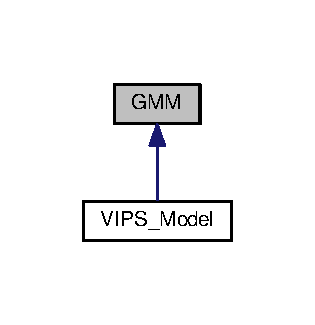
\includegraphics[width=151pt]{classGMM__inherit__graph}
\end{center}
\end{figure}
\subsection*{Public Member Functions}
\begin{DoxyCompactItemize}
\item 
\hyperlink{classGMM_a84d95fb2c6582568a9d9a1b0efe200a4}{G\+MM} (int dim, int max\+\_\+components=100000)
\item 
arma\+::cube \hyperlink{classGMM_acd0dd8e7f38a792f515d296dd467924a}{interpolate\+\_\+covs\+\_\+for\+\_\+query\+\_\+points} (mat query\+\_\+points)
\item 
virtual void \hyperlink{classGMM_a00680c4a0c5f3befd742015bb8ad0a08}{add\+\_\+components\+\_\+at\+\_\+locations} (mat means)
\item 
virtual void \hyperlink{classGMM_ae33b6f52e8585c0cd590fd1d509956b0}{add\+\_\+components} (mat means, cube covs)
\item 
virtual void \hyperlink{classGMM_a07d7ade16c34458f6cf8fad958728c98}{add\+\_\+components\+\_\+inv\+Chols} (mat new\+\_\+means, cube new\+\_\+inv\+Chols)
\item 
void \hyperlink{classGMM_a82a84a6ad3ca8f5943b2ecaece9b6d1c}{delete\+\_\+components} (uvec indices)
\item 
virtual void \hyperlink{classGMM_a25c1ccd0c99b1ebd1e36592b912e74c2}{delete\+\_\+component} (int index)
\item 
void \hyperlink{classGMM_a929918e74c549b6ccca8c3cc246cd809}{prune\+\_\+to\+\_\+max\+\_\+components} (uvec protected\+\_\+components)
\item 
void \hyperlink{classGMM_a95ec14bd0e19af434ecb7b892288c6de}{change\+Component} (int index, mat new\+Chol, vec new\+Mean)
\item 
vec \hyperlink{classGMM_abcf7aa873a9bc0df374ff1284de786bc}{compute\+\_\+component\+\_\+densities} (int idx, mat samples, bool return\+\_\+log)
\item 
std\+::tuple$<$ mat, mat $>$ \hyperlink{classGMM_a8a9e502395f9d7f6a63eb7f56df5a73f}{compute\+\_\+joint\+\_\+densities} (mat samples, bool return\+\_\+log)
\item 
vec \hyperlink{classGMM_a1c2d04636a640ce56bf245df750e97ea}{evaluate\+\_\+\+G\+M\+M\+\_\+densities} (mat samples, bool return\+\_\+log)
\item 
vec \hyperlink{classGMM_a9a0e20b34d77c21fb31449dac5d1bd32}{evaluate\+\_\+\+G\+M\+M\+\_\+densities\+\_\+low\+\_\+mem} (mat samples)
\item 
std\+::tuple$<$ mat, mat, rowvec, rowvec, vec, mat $>$ \hyperlink{classGMM_a11d50f8336e3f0b4371fa4c7c023e11f}{compute\+\_\+log\+\_\+marginals} (mat samples)
\item 
std\+::tuple$<$ mat, rowvec, rowvec, vec, mat $>$ \hyperlink{classGMM_a03b69ac93de1b177102fc9378665f20b}{compute\+\_\+log\+\_\+marginals\+\_\+from\+\_\+comp\+\_\+densities} (mat log\+\_\+component\+\_\+marginals)
\item 
mat \hyperlink{classGMM_a5e5c1278fc67c3cb4b5cdeeb9390ab98}{sample\+\_\+from\+\_\+component} (int index, int n)
\item 
std\+::tuple$<$ mat, uvec $>$ \hyperlink{classGMM_ad7687ba93ab195673c26d02690d14d27}{sample\+\_\+from\+\_\+mixture\+\_\+weights} (double N, vec new\+\_\+weigths)
\item 
std\+::tuple$<$ mat, uvec $>$ \hyperlink{classGMM_afb3f91ba6e939739198a49c85c92ace4}{sample\+\_\+from\+\_\+mixture} (int n, double temperature=1.\+0)
\item 
void {\bfseries set\+Weights} (vec new\+\_\+weights)\hypertarget{classGMM_a1326b4c55a66445adb3888d1a77bb2cb}{}\label{classGMM_a1326b4c55a66445adb3888d1a77bb2cb}

\item 
void {\bfseries set\+Weights} (vec new\+\_\+weights, vec new\+\_\+log\+\_\+weights)\hypertarget{classGMM_a79c00e9de57111610b41fd98577b7b6a}{}\label{classGMM_a79c00e9de57111610b41fd98577b7b6a}

\item 
mat {\bfseries get\+Means} ()\hypertarget{classGMM_ae14f838f611896e02074e897247f461b}{}\label{classGMM_ae14f838f611896e02074e897247f461b}

\item 
mat {\bfseries get\+Means} (uvec indices)\hypertarget{classGMM_adeb0e2fd08493b3fd182286566a27a89}{}\label{classGMM_adeb0e2fd08493b3fd182286566a27a89}

\item 
cube {\bfseries get\+Covs} ()\hypertarget{classGMM_a88fd853731318d167e32b220debcf3c8}{}\label{classGMM_a88fd853731318d167e32b220debcf3c8}

\item 
cube {\bfseries get\+Chols} ()\hypertarget{classGMM_a84da191cb14375e572f192322b35ac6a}{}\label{classGMM_a84da191cb14375e572f192322b35ac6a}

\item 
cube {\bfseries get\+Inv\+Chols} ()\hypertarget{classGMM_a0cede71e7f6fb12cc7710567a3f4feef}{}\label{classGMM_a0cede71e7f6fb12cc7710567a3f4feef}

\item 
vec {\bfseries get\+Weights} ()\hypertarget{classGMM_a23d3f84a62535b3fbb3ef5cf9385f58b}{}\label{classGMM_a23d3f84a62535b3fbb3ef5cf9385f58b}

\item 
vec {\bfseries get\+Log\+Weights} ()\hypertarget{classGMM_a56ffba07ec2803f25444592f275b3d31}{}\label{classGMM_a56ffba07ec2803f25444592f275b3d31}

\item 
vec {\bfseries get\+Entropies} ()\hypertarget{classGMM_a9c9d5c5fa14d84de0a0d0fd249cf705e}{}\label{classGMM_a9c9d5c5fa14d84de0a0d0fd249cf705e}

\item 
vec {\bfseries get\+Determinants} ()\hypertarget{classGMM_a060c1a9c7a363ce01d7220500fc1db2d}{}\label{classGMM_a060c1a9c7a363ce01d7220500fc1db2d}

\item 
int {\bfseries get\+Num\+Components} ()\hypertarget{classGMM_a0db6332cddaa01a06caafada3c6354c7}{}\label{classGMM_a0db6332cddaa01a06caafada3c6354c7}

\item 
int {\bfseries get\+Num\+Dimensions} ()\hypertarget{classGMM_a6e11a4916285155c0acb69beb02560bd}{}\label{classGMM_a6e11a4916285155c0acb69beb02560bd}

\end{DoxyCompactItemize}
\subsection*{Public Attributes}
\begin{DoxyCompactItemize}
\item 
int {\bfseries max\+\_\+components}\hypertarget{classGMM_af0c5335a6c9ac80c07d3212314e0d8b6}{}\label{classGMM_af0c5335a6c9ac80c07d3212314e0d8b6}

\end{DoxyCompactItemize}
\subsection*{Protected Member Functions}
\begin{DoxyCompactItemize}
\item 
std\+::tuple$<$ vec, vec, vec $>$ \hyperlink{classGMM_adfbd4c7449817315f02f54736751e1ce}{soft\+Max\+\_\+2D} (mat data)
\end{DoxyCompactItemize}
\subsection*{Protected Attributes}
\begin{DoxyCompactItemize}
\item 
double {\bfseries entropy\+\_\+offset}\hypertarget{classGMM_afbdca4e356f354e6ab36c2975aa7ae94}{}\label{classGMM_afbdca4e356f354e6ab36c2975aa7ae94}

\item 
int {\bfseries dim}\hypertarget{classGMM_a94d1cbf3cd1c15b81d2ac5809273304a}{}\label{classGMM_a94d1cbf3cd1c15b81d2ac5809273304a}

\item 
int {\bfseries num\+\_\+components}\hypertarget{classGMM_afa64fb9b37cff173b5ad1105c34abb2b}{}\label{classGMM_afa64fb9b37cff173b5ad1105c34abb2b}

\item 
mat {\bfseries means}\hypertarget{classGMM_ae8876c900c276e64c75ba799354fc46b}{}\label{classGMM_ae8876c900c276e64c75ba799354fc46b}

\item 
cube {\bfseries covs}\hypertarget{classGMM_abb060a06a7d148fb220ba3524030b7c9}{}\label{classGMM_abb060a06a7d148fb220ba3524030b7c9}

\item 
cube {\bfseries chols}\hypertarget{classGMM_ad6b6fd943a44e972792b01db68042eec}{}\label{classGMM_ad6b6fd943a44e972792b01db68042eec}

\item 
cube {\bfseries inv\+\_\+chols}\hypertarget{classGMM_a2b50c3568e366f5f774b2f73bb239977}{}\label{classGMM_a2b50c3568e366f5f774b2f73bb239977}

\item 
vec {\bfseries weights}\hypertarget{classGMM_ac92b4a601ede428eb4a6b20c9be252d9}{}\label{classGMM_ac92b4a601ede428eb4a6b20c9be252d9}

\item 
vec {\bfseries log\+\_\+weights}\hypertarget{classGMM_abfa4ad63087bb64e6324c231ad88478a}{}\label{classGMM_abfa4ad63087bb64e6324c231ad88478a}

\item 
vec {\bfseries entropies}\hypertarget{classGMM_a7b6ae5a12e6230d7a8ad06f6c86fb247}{}\label{classGMM_a7b6ae5a12e6230d7a8ad06f6c86fb247}

\item 
vec {\bfseries determinants}\hypertarget{classGMM_a18bbf0ad6127d7cd8f65fc688030d830}{}\label{classGMM_a18bbf0ad6127d7cd8f65fc688030d830}

\item 
std\+::default\+\_\+random\+\_\+engine {\bfseries rng}\hypertarget{classGMM_a6a5f6bf173dea2faf179b75065d1b806}{}\label{classGMM_a6a5f6bf173dea2faf179b75065d1b806}

\end{DoxyCompactItemize}


\subsection{Constructor \& Destructor Documentation}
\index{G\+MM@{G\+MM}!G\+MM@{G\+MM}}
\index{G\+MM@{G\+MM}!G\+MM@{G\+MM}}
\subsubsection[{\texorpdfstring{G\+M\+M(int dim, int max\+\_\+components=100000)}{GMM(int dim, int max_components=100000)}}]{\setlength{\rightskip}{0pt plus 5cm}G\+M\+M\+::\+G\+MM (
\begin{DoxyParamCaption}
\item[{int}]{dim, }
\item[{int}]{max\+\_\+components = {\ttfamily 100000}}
\end{DoxyParamCaption}
)}\hypertarget{classGMM_a84d95fb2c6582568a9d9a1b0efe200a4}{}\label{classGMM_a84d95fb2c6582568a9d9a1b0efe200a4}
A Gaussian Mixture Model. 
\begin{DoxyParams}{Parameters}
{\em dim} & the number of dimensions \\
\hline
{\em max\+\_\+components} & maximum number of components this \hyperlink{classGMM}{G\+MM} may comprise \\
\hline
\end{DoxyParams}


\subsection{Member Function Documentation}
\index{G\+MM@{G\+MM}!add\+\_\+components@{add\+\_\+components}}
\index{add\+\_\+components@{add\+\_\+components}!G\+MM@{G\+MM}}
\subsubsection[{\texorpdfstring{add\+\_\+components(mat means, cube covs)}{add_components(mat means, cube covs)}}]{\setlength{\rightskip}{0pt plus 5cm}void G\+M\+M\+::add\+\_\+components (
\begin{DoxyParamCaption}
\item[{mat}]{new\+\_\+means, }
\item[{cube}]{new\+\_\+covs}
\end{DoxyParamCaption}
)\hspace{0.3cm}{\ttfamily [virtual]}}\hypertarget{classGMM_ae33b6f52e8585c0cd590fd1d509956b0}{}\label{classGMM_ae33b6f52e8585c0cd590fd1d509956b0}
Adds new components. The weights will be initialized close to zero. 
\begin{DoxyParams}{Parameters}
{\em new\+\_\+means} & -\/ matrix of size N\+\_\+dimensions x N\+\_\+new\+Components specifying the means of the new components \\
\hline
{\em new\+\_\+covs} & -\/ cube of size N\+\_\+dimensions x N\+\_\+dimensions x N\+\_\+new\+Components specifying the covariance matrices of the new components \\
\hline
\end{DoxyParams}
\index{G\+MM@{G\+MM}!add\+\_\+components\+\_\+at\+\_\+locations@{add\+\_\+components\+\_\+at\+\_\+locations}}
\index{add\+\_\+components\+\_\+at\+\_\+locations@{add\+\_\+components\+\_\+at\+\_\+locations}!G\+MM@{G\+MM}}
\subsubsection[{\texorpdfstring{add\+\_\+components\+\_\+at\+\_\+locations(mat means)}{add_components_at_locations(mat means)}}]{\setlength{\rightskip}{0pt plus 5cm}void G\+M\+M\+::add\+\_\+components\+\_\+at\+\_\+locations (
\begin{DoxyParamCaption}
\item[{mat}]{new\+\_\+means}
\end{DoxyParamCaption}
)\hspace{0.3cm}{\ttfamily [virtual]}}\hypertarget{classGMM_a00680c4a0c5f3befd742015bb8ad0a08}{}\label{classGMM_a00680c4a0c5f3befd742015bb8ad0a08}
Creates new components on the given positions.~\newline
 The covariance matrices are initialized by interpolating the covariance matrices of the existing components weighted by their responsibilities for the new mean.~\newline
 The weights are initialized to low values, such that the change of the mixture is negligible 
\begin{DoxyParams}{Parameters}
{\em means} & -\/ matrix of size N\+\_\+dimensions x N\+\_\+new\+Components specifying at which positions new components are to be added \\
\hline
\end{DoxyParams}
\index{G\+MM@{G\+MM}!add\+\_\+components\+\_\+inv\+Chols@{add\+\_\+components\+\_\+inv\+Chols}}
\index{add\+\_\+components\+\_\+inv\+Chols@{add\+\_\+components\+\_\+inv\+Chols}!G\+MM@{G\+MM}}
\subsubsection[{\texorpdfstring{add\+\_\+components\+\_\+inv\+Chols(mat new\+\_\+means, cube new\+\_\+inv\+Chols)}{add_components_invChols(mat new_means, cube new_invChols)}}]{\setlength{\rightskip}{0pt plus 5cm}void G\+M\+M\+::add\+\_\+components\+\_\+inv\+Chols (
\begin{DoxyParamCaption}
\item[{mat}]{new\+\_\+means, }
\item[{cube}]{new\+\_\+inv\+Chols}
\end{DoxyParamCaption}
)\hspace{0.3cm}{\ttfamily [virtual]}}\hypertarget{classGMM_a07d7ade16c34458f6cf8fad958728c98}{}\label{classGMM_a07d7ade16c34458f6cf8fad958728c98}
Adds new components. Second parameter is interpreted as inverse cholesky matrix. The weights will be initialized close to zero 
\begin{DoxyParams}{Parameters}
{\em new\+\_\+means} & -\/ matrix of size N\+\_\+dimensions x N\+\_\+new\+Components specifying the means of the new components \\
\hline
{\em new\+\_\+\+Inv\+Chols} & -\/ cube of size N\+\_\+dimensions x N\+\_\+dimensions x N\+\_\+new\+Components specifying the inverse cholesky matrices of the new components \\
\hline
\end{DoxyParams}
\index{G\+MM@{G\+MM}!change\+Component@{change\+Component}}
\index{change\+Component@{change\+Component}!G\+MM@{G\+MM}}
\subsubsection[{\texorpdfstring{change\+Component(int index, mat new\+Chol, vec new\+Mean)}{changeComponent(int index, mat newChol, vec newMean)}}]{\setlength{\rightskip}{0pt plus 5cm}void G\+M\+M\+::change\+Component (
\begin{DoxyParamCaption}
\item[{int}]{index, }
\item[{mat}]{new\+Chol, }
\item[{vec}]{new\+Mean}
\end{DoxyParamCaption}
)}\hypertarget{classGMM_a95ec14bd0e19af434ecb7b892288c6de}{}\label{classGMM_a95ec14bd0e19af434ecb7b892288c6de}
Change the Mean and Covariance of the specified component 
\begin{DoxyParams}{Parameters}
{\em index} & -\/ an index specifying which component to modify \\
\hline
{\em new\+Chol} & -\/ new cholesky decomposition of the covariance matrix \\
\hline
{\em new\+Mean} & -\/ new mean \\
\hline
\end{DoxyParams}
\index{G\+MM@{G\+MM}!compute\+\_\+component\+\_\+densities@{compute\+\_\+component\+\_\+densities}}
\index{compute\+\_\+component\+\_\+densities@{compute\+\_\+component\+\_\+densities}!G\+MM@{G\+MM}}
\subsubsection[{\texorpdfstring{compute\+\_\+component\+\_\+densities(int idx, mat samples, bool return\+\_\+log)}{compute_component_densities(int idx, mat samples, bool return_log)}}]{\setlength{\rightskip}{0pt plus 5cm}vec G\+M\+M\+::compute\+\_\+component\+\_\+densities (
\begin{DoxyParamCaption}
\item[{int}]{idx, }
\item[{mat}]{samples, }
\item[{bool}]{return\+\_\+log}
\end{DoxyParamCaption}
)}\hypertarget{classGMM_abcf7aa873a9bc0df374ff1284de786bc}{}\label{classGMM_abcf7aa873a9bc0df374ff1284de786bc}
Evaluates the given query samples on the given component. \begin{DoxyReturn}{Returns}
a vector of size num\+\_\+samples containing p(s$\vert$o\+\_\+idx) 
\end{DoxyReturn}
\index{G\+MM@{G\+MM}!compute\+\_\+joint\+\_\+densities@{compute\+\_\+joint\+\_\+densities}}
\index{compute\+\_\+joint\+\_\+densities@{compute\+\_\+joint\+\_\+densities}!G\+MM@{G\+MM}}
\subsubsection[{\texorpdfstring{compute\+\_\+joint\+\_\+densities(mat samples, bool return\+\_\+log)}{compute_joint_densities(mat samples, bool return_log)}}]{\setlength{\rightskip}{0pt plus 5cm}std\+::tuple$<$ mat, mat $>$ G\+M\+M\+::compute\+\_\+joint\+\_\+densities (
\begin{DoxyParamCaption}
\item[{mat}]{samples, }
\item[{bool}]{return\+\_\+log}
\end{DoxyParamCaption}
)}\hypertarget{classGMM_a8a9e502395f9d7f6a63eb7f56df5a73f}{}\label{classGMM_a8a9e502395f9d7f6a63eb7f56df5a73f}
evaluates all components on the given samples. \begin{DoxyReturn}{Returns}
a tuple of two matrices with size num\+\_\+components X num\+\_\+samples~\newline
 tuple\mbox{[}0\mbox{]} contains the joint densities p(s,o)~\newline
 tuple\mbox{[}1\mbox{]} contains the marginal densities p(s$\vert$o) 
\end{DoxyReturn}
\index{G\+MM@{G\+MM}!compute\+\_\+log\+\_\+marginals@{compute\+\_\+log\+\_\+marginals}}
\index{compute\+\_\+log\+\_\+marginals@{compute\+\_\+log\+\_\+marginals}!G\+MM@{G\+MM}}
\subsubsection[{\texorpdfstring{compute\+\_\+log\+\_\+marginals(mat samples)}{compute_log_marginals(mat samples)}}]{\setlength{\rightskip}{0pt plus 5cm}std\+::tuple$<$ mat, mat, rowvec, rowvec, vec, mat $>$ G\+M\+M\+::compute\+\_\+log\+\_\+marginals (
\begin{DoxyParamCaption}
\item[{mat}]{samples}
\end{DoxyParamCaption}
)}\hypertarget{classGMM_a11d50f8336e3f0b4371fa4c7c023e11f}{}\label{classGMM_a11d50f8336e3f0b4371fa4c7c023e11f}
This function mainly computes the log\+\_\+responsibilities \mbox{[}log(p(comp$\vert$sample))\mbox{]} and the the log densities \mbox{[}log(\+G\+M\+M(samples))\mbox{]}. However, intermediate computations are returned as well, as they are required for efficient computation.~\newline
 For example, when recomputing the log\+\_\+responsibilites in a numerical stable way after adding more samples, tuple\mbox{[}2\mbox{]} and tuple\mbox{[}3\mbox{]} can be exploited to avoid unnecessary computations.


\begin{DoxyParams}{Parameters}
{\em samples,a} & matrix N\+\_\+\+Dim x N\+\_\+\+Samples containing the samples to be evaluated \\
\hline
\end{DoxyParams}
\begin{DoxyReturn}{Returns}
a tuple, such that~\newline
 tuple\mbox{[}0\mbox{]}\+: a matrix N\+\_\+\+Components x N\+\_\+\+Samples containing the log of joint densities log(p(s,o))~\newline
 tuple\mbox{[}1\mbox{]}\+: a matrix N\+\_\+\+Components x N\+\_\+\+Samples containing the log of component marginals log(p(s$\vert$o))~\newline
 tuple\mbox{[}2\mbox{]}\+: a row-\/vector containing column-\/wise, negated maxima of tuple\mbox{[}1\mbox{]}~\newline
 tuple\mbox{[}3\mbox{]}\+: a row-\/vector containing the column-\/wise summations, sum(exp(log(tuple\mbox{[}1\mbox{]}+tuple\mbox{[}2\mbox{]}))~\newline
 tuple\mbox{[}4\mbox{]}\+: a vector containing the \hyperlink{classGMM}{G\+MM} log densities for each sample (log(tuple\mbox{[}3\mbox{]}) -\/ tuple\mbox{[}2\mbox{]}, i.\+e. log(p(s))~\newline
 tuple\mbox{[}5\mbox{]}\+: a matrix containing the log responsibilities (row-\/wise subtraction of tuple\mbox{[}4\mbox{]} from tuple\mbox{[}2\mbox{]}, i.\+e. p(o$\vert$s)) 
\end{DoxyReturn}
\index{G\+MM@{G\+MM}!compute\+\_\+log\+\_\+marginals\+\_\+from\+\_\+comp\+\_\+densities@{compute\+\_\+log\+\_\+marginals\+\_\+from\+\_\+comp\+\_\+densities}}
\index{compute\+\_\+log\+\_\+marginals\+\_\+from\+\_\+comp\+\_\+densities@{compute\+\_\+log\+\_\+marginals\+\_\+from\+\_\+comp\+\_\+densities}!G\+MM@{G\+MM}}
\subsubsection[{\texorpdfstring{compute\+\_\+log\+\_\+marginals\+\_\+from\+\_\+comp\+\_\+densities(mat log\+\_\+component\+\_\+marginals)}{compute_log_marginals_from_comp_densities(mat log_component_marginals)}}]{\setlength{\rightskip}{0pt plus 5cm}std\+::tuple$<$ mat, rowvec, rowvec, vec, mat $>$ G\+M\+M\+::compute\+\_\+log\+\_\+marginals\+\_\+from\+\_\+comp\+\_\+densities (
\begin{DoxyParamCaption}
\item[{mat}]{log\+\_\+component\+\_\+marginals}
\end{DoxyParamCaption}
)}\hypertarget{classGMM_a03b69ac93de1b177102fc9378665f20b}{}\label{classGMM_a03b69ac93de1b177102fc9378665f20b}
This function mainly computes the log\+\_\+responsibilities \mbox{[}log(p(comp$\vert$sample))\mbox{]} and the the log densities \mbox{[}log(\+G\+M\+M(samples))\mbox{]}. However, intermediate computations are returned as well, as they are required for efficient computation.~\newline
 For example, when recomputing the log\+\_\+responsibilites in a numerical stable way after adding more samples, tuple\mbox{[}1\mbox{]} and tuple\mbox{[}2\mbox{]} can be exploited to avoid unnecessary computations.


\begin{DoxyParams}{Parameters}
{\em log\+\_\+component\+\_\+marginals,a} & matrix N\+\_\+\+Components x N\+\_\+\+Samples containing the log of component marginals log(p(s$\vert$o)) \\
\hline
\end{DoxyParams}
\begin{DoxyReturn}{Returns}
a tuple, such that~\newline
 tuple\mbox{[}0\mbox{]}\+: a matrix N\+\_\+\+Components x N\+\_\+\+Samples containing the log of joint densities log(p(s,o))~\newline
 tuple\mbox{[}1\mbox{]}\+: a row-\/vector containing column-\/wise, negated maxima of tuple\mbox{[}0\mbox{]}~\newline
 tuple\mbox{[}2\mbox{]}\+: a row-\/vector containing the column-\/wise summations, sum(exp(log(tuple\mbox{[}0\mbox{]}+tuple\mbox{[}1\mbox{]}))~\newline
 tuple\mbox{[}3\mbox{]}\+: a vector containing the \hyperlink{classGMM}{G\+MM} log densities for each sample (log(tuple\mbox{[}2\mbox{]}) -\/ tuple\mbox{[}1\mbox{]}, i.\+e. log(p(s))~\newline
 tuple\mbox{[}4\mbox{]}\+: a matrix containing the log responsibilities (row-\/wise subtraction of tuple\mbox{[}3\mbox{]} from tuple\mbox{[}1\mbox{]}, i.\+e. p(o$\vert$s)) 
\end{DoxyReturn}
\index{G\+MM@{G\+MM}!delete\+\_\+component@{delete\+\_\+component}}
\index{delete\+\_\+component@{delete\+\_\+component}!G\+MM@{G\+MM}}
\subsubsection[{\texorpdfstring{delete\+\_\+component(int index)}{delete_component(int index)}}]{\setlength{\rightskip}{0pt plus 5cm}void G\+M\+M\+::delete\+\_\+component (
\begin{DoxyParamCaption}
\item[{int}]{index}
\end{DoxyParamCaption}
)\hspace{0.3cm}{\ttfamily [virtual]}}\hypertarget{classGMM_a25c1ccd0c99b1ebd1e36592b912e74c2}{}\label{classGMM_a25c1ccd0c99b1ebd1e36592b912e74c2}
Delete a single componentent and renormalize the weights afterwards. 
\begin{DoxyParams}{Parameters}
{\em index} & specifying which component to delete \\
\hline
\end{DoxyParams}


Reimplemented in \hyperlink{classVIPS__Model_a6b0edde4a9a744639e1588cff6a5fa23}{V\+I\+P\+S\+\_\+\+Model}.

\index{G\+MM@{G\+MM}!delete\+\_\+components@{delete\+\_\+components}}
\index{delete\+\_\+components@{delete\+\_\+components}!G\+MM@{G\+MM}}
\subsubsection[{\texorpdfstring{delete\+\_\+components(uvec indices)}{delete_components(uvec indices)}}]{\setlength{\rightskip}{0pt plus 5cm}void G\+M\+M\+::delete\+\_\+components (
\begin{DoxyParamCaption}
\item[{uvec}]{indices}
\end{DoxyParamCaption}
)}\hypertarget{classGMM_a82a84a6ad3ca8f5943b2ecaece9b6d1c}{}\label{classGMM_a82a84a6ad3ca8f5943b2ecaece9b6d1c}
Delete the components given by the indices and renormalize the weights afterwards. 
\begin{DoxyParams}{Parameters}
{\em indices} & specifying which component to delete \\
\hline
\end{DoxyParams}
\index{G\+MM@{G\+MM}!evaluate\+\_\+\+G\+M\+M\+\_\+densities@{evaluate\+\_\+\+G\+M\+M\+\_\+densities}}
\index{evaluate\+\_\+\+G\+M\+M\+\_\+densities@{evaluate\+\_\+\+G\+M\+M\+\_\+densities}!G\+MM@{G\+MM}}
\subsubsection[{\texorpdfstring{evaluate\+\_\+\+G\+M\+M\+\_\+densities(mat samples, bool return\+\_\+log)}{evaluate_GMM_densities(mat samples, bool return_log)}}]{\setlength{\rightskip}{0pt plus 5cm}vec G\+M\+M\+::evaluate\+\_\+\+G\+M\+M\+\_\+densities (
\begin{DoxyParamCaption}
\item[{mat}]{samples, }
\item[{bool}]{return\+\_\+log}
\end{DoxyParamCaption}
)}\hypertarget{classGMM_a1c2d04636a640ce56bf245df750e97ea}{}\label{classGMM_a1c2d04636a640ce56bf245df750e97ea}
Evaluates the \hyperlink{classGMM}{G\+MM} on the given samples. \begin{DoxyReturn}{Returns}
a vector of size num\+\_\+samples containing p(s) 
\end{DoxyReturn}
\index{G\+MM@{G\+MM}!evaluate\+\_\+\+G\+M\+M\+\_\+densities\+\_\+low\+\_\+mem@{evaluate\+\_\+\+G\+M\+M\+\_\+densities\+\_\+low\+\_\+mem}}
\index{evaluate\+\_\+\+G\+M\+M\+\_\+densities\+\_\+low\+\_\+mem@{evaluate\+\_\+\+G\+M\+M\+\_\+densities\+\_\+low\+\_\+mem}!G\+MM@{G\+MM}}
\subsubsection[{\texorpdfstring{evaluate\+\_\+\+G\+M\+M\+\_\+densities\+\_\+low\+\_\+mem(mat samples)}{evaluate_GMM_densities_low_mem(mat samples)}}]{\setlength{\rightskip}{0pt plus 5cm}vec G\+M\+M\+::evaluate\+\_\+\+G\+M\+M\+\_\+densities\+\_\+low\+\_\+mem (
\begin{DoxyParamCaption}
\item[{mat}]{samples}
\end{DoxyParamCaption}
)}\hypertarget{classGMM_a9a0e20b34d77c21fb31449dac5d1bd32}{}\label{classGMM_a9a0e20b34d77c21fb31449dac5d1bd32}
Evaluates the \hyperlink{classGMM}{G\+MM} on the given samples in a memory efficient way. This function is recommended for very large number of samples or components 
\begin{DoxyParams}{Parameters}
{\em samples} & -\/ a matrix of size N\+\_\+dim x N\+\_\+samples of samples to be evaluated \\
\hline
\end{DoxyParams}
\begin{DoxyReturn}{Returns}
the log \hyperlink{classGMM}{G\+MM} densities log(p(s)) 
\end{DoxyReturn}
\index{G\+MM@{G\+MM}!interpolate\+\_\+covs\+\_\+for\+\_\+query\+\_\+points@{interpolate\+\_\+covs\+\_\+for\+\_\+query\+\_\+points}}
\index{interpolate\+\_\+covs\+\_\+for\+\_\+query\+\_\+points@{interpolate\+\_\+covs\+\_\+for\+\_\+query\+\_\+points}!G\+MM@{G\+MM}}
\subsubsection[{\texorpdfstring{interpolate\+\_\+covs\+\_\+for\+\_\+query\+\_\+points(mat query\+\_\+points)}{interpolate_covs_for_query_points(mat query_points)}}]{\setlength{\rightskip}{0pt plus 5cm}cube G\+M\+M\+::interpolate\+\_\+covs\+\_\+for\+\_\+query\+\_\+points (
\begin{DoxyParamCaption}
\item[{mat}]{query\+\_\+points}
\end{DoxyParamCaption}
)}\hypertarget{classGMM_acd0dd8e7f38a792f515d296dd467924a}{}\label{classGMM_acd0dd8e7f38a792f515d296dd467924a}
Compute a covariance matrix for each given query point by interpolating the covariance matrices of the \hyperlink{classGMM}{G\+MM} components weighted by the their responsibility for the given query point.~\newline
 This can be used, for example, for initializing new components.~\newline
 
\begin{DoxyParams}{Parameters}
{\em query\+\_\+points} & -\/ D X N matrix containing the query points \\
\hline
\end{DoxyParams}
\begin{DoxyReturn}{Returns}
a cube of size N x D X D containing the covariance matrices 
\end{DoxyReturn}
\index{G\+MM@{G\+MM}!prune\+\_\+to\+\_\+max\+\_\+components@{prune\+\_\+to\+\_\+max\+\_\+components}}
\index{prune\+\_\+to\+\_\+max\+\_\+components@{prune\+\_\+to\+\_\+max\+\_\+components}!G\+MM@{G\+MM}}
\subsubsection[{\texorpdfstring{prune\+\_\+to\+\_\+max\+\_\+components(uvec protected\+\_\+components)}{prune_to_max_components(uvec protected_components)}}]{\setlength{\rightskip}{0pt plus 5cm}void G\+M\+M\+::prune\+\_\+to\+\_\+max\+\_\+components (
\begin{DoxyParamCaption}
\item[{uvec}]{protected\+\_\+components}
\end{DoxyParamCaption}
)}\hypertarget{classGMM_a929918e74c549b6ccca8c3cc246cd809}{}\label{classGMM_a929918e74c549b6ccca8c3cc246cd809}
If the \hyperlink{classGMM}{G\+MM} currently contains more than max\+\_\+components, removes the N=(num\+\_\+components -\/ max\+\_\+components) components with lowest weight. However, does not delete components with an index that is contained in protected\+\_\+components. 
\begin{DoxyParams}{Parameters}
{\em protected\+\_\+components} & -\/ indices of such components that should not be deleted. \\
\hline
\end{DoxyParams}
\index{G\+MM@{G\+MM}!sample\+\_\+from\+\_\+component@{sample\+\_\+from\+\_\+component}}
\index{sample\+\_\+from\+\_\+component@{sample\+\_\+from\+\_\+component}!G\+MM@{G\+MM}}
\subsubsection[{\texorpdfstring{sample\+\_\+from\+\_\+component(int index, int n)}{sample_from_component(int index, int n)}}]{\setlength{\rightskip}{0pt plus 5cm}mat G\+M\+M\+::sample\+\_\+from\+\_\+component (
\begin{DoxyParamCaption}
\item[{int}]{index, }
\item[{int}]{n}
\end{DoxyParamCaption}
)}\hypertarget{classGMM_a5e5c1278fc67c3cb4b5cdeeb9390ab98}{}\label{classGMM_a5e5c1278fc67c3cb4b5cdeeb9390ab98}
Draw n samples from the specified component \index{G\+MM@{G\+MM}!sample\+\_\+from\+\_\+mixture@{sample\+\_\+from\+\_\+mixture}}
\index{sample\+\_\+from\+\_\+mixture@{sample\+\_\+from\+\_\+mixture}!G\+MM@{G\+MM}}
\subsubsection[{\texorpdfstring{sample\+\_\+from\+\_\+mixture(int n, double temperature=1.\+0)}{sample_from_mixture(int n, double temperature=1.0)}}]{\setlength{\rightskip}{0pt plus 5cm}std\+::tuple$<$ mat, uvec $>$ G\+M\+M\+::sample\+\_\+from\+\_\+mixture (
\begin{DoxyParamCaption}
\item[{int}]{n, }
\item[{double}]{temperature = {\ttfamily 1.0}}
\end{DoxyParamCaption}
)}\hypertarget{classGMM_afb3f91ba6e939739198a49c85c92ace4}{}\label{classGMM_afb3f91ba6e939739198a49c85c92ace4}
Return samples and the corresponding indices of the components. temperature can be used to scale the weights \index{G\+MM@{G\+MM}!sample\+\_\+from\+\_\+mixture\+\_\+weights@{sample\+\_\+from\+\_\+mixture\+\_\+weights}}
\index{sample\+\_\+from\+\_\+mixture\+\_\+weights@{sample\+\_\+from\+\_\+mixture\+\_\+weights}!G\+MM@{G\+MM}}
\subsubsection[{\texorpdfstring{sample\+\_\+from\+\_\+mixture\+\_\+weights(double N, vec new\+\_\+weigths)}{sample_from_mixture_weights(double N, vec new_weigths)}}]{\setlength{\rightskip}{0pt plus 5cm}std\+::tuple$<$ mat, uvec $>$ G\+M\+M\+::sample\+\_\+from\+\_\+mixture\+\_\+weights (
\begin{DoxyParamCaption}
\item[{double}]{N, }
\item[{vec}]{new\+\_\+weights}
\end{DoxyParamCaption}
)}\hypertarget{classGMM_ad7687ba93ab195673c26d02690d14d27}{}\label{classGMM_ad7687ba93ab195673c26d02690d14d27}
Sample from the current \hyperlink{classGMM}{G\+MM}, but use the specified the given component coefficient. 
\begin{DoxyParams}{Parameters}
{\em N} & -\/ the numb er of samples to been drawn \\
\hline
{\em weights} & -\/ the weights (coefficients) to be used \\
\hline
\end{DoxyParams}
\begin{DoxyReturn}{Returns}
samples -\/ N Samples drwan from the mixture with the given weights 

indices -\/ for each sample, the index of the component that was used for drawing it 
\end{DoxyReturn}
\index{G\+MM@{G\+MM}!soft\+Max\+\_\+2D@{soft\+Max\+\_\+2D}}
\index{soft\+Max\+\_\+2D@{soft\+Max\+\_\+2D}!G\+MM@{G\+MM}}
\subsubsection[{\texorpdfstring{soft\+Max\+\_\+2\+D(mat data)}{softMax_2D(mat data)}}]{\setlength{\rightskip}{0pt plus 5cm}std\+::tuple$<$ vec, vec, vec $>$ G\+M\+M\+::soft\+Max\+\_\+2D (
\begin{DoxyParamCaption}
\item[{mat}]{data}
\end{DoxyParamCaption}
)\hspace{0.3cm}{\ttfamily [protected]}}\hypertarget{classGMM_adfbd4c7449817315f02f54736751e1ce}{}\label{classGMM_adfbd4c7449817315f02f54736751e1ce}
computes log(sum(exp(data))) columnwise \begin{DoxyReturn}{Returns}
a tuple containing~\newline
 tuple\mbox{[}0\mbox{]}\+: a vector containing the column-\/wise softmaxs, max(data) + log(sum(exp(data-\/max(data)))~\newline
 tuple\mbox{[}1\mbox{]}\+: a vector containing column-\/wise offsets, i.\+e. -\/max(data)~\newline
 tuple\mbox{[}2\mbox{]}\+: a vector containing the column-\/wise summations, sum(exp(data-\/max(data))) 
\end{DoxyReturn}


The documentation for this class was generated from the following files\+:\begin{DoxyCompactItemize}
\item 
G\+M\+M.\+h\item 
G\+M\+M.\+cpp\end{DoxyCompactItemize}

\hypertarget{classMMD}{}\section{M\+MD Class Reference}
\label{classMMD}\index{M\+MD@{M\+MD}}
\subsection*{Public Member Functions}
\begin{DoxyCompactItemize}
\item 
{\bfseries M\+MD} (double $\ast$samples\+\_\+ptr, int samples\+\_\+dim1, int samples\+\_\+dim2)\hypertarget{classMMD_a9fa2c3a131f1028c8d8482cd3f481188}{}\label{classMMD_a9fa2c3a131f1028c8d8482cd3f481188}

\item 
void {\bfseries estimate\+\_\+median} (int max\+\_\+points\+\_\+for\+\_\+median)\hypertarget{classMMD_a3fccd3ddfd019c5dd835b09157734f7d}{}\label{classMMD_a3fccd3ddfd019c5dd835b09157734f7d}

\item 
void {\bfseries get\+\_\+median} (double $\ast$$\ast$median\+\_\+out\+\_\+ptr, int $\ast$median\+\_\+out\+\_\+dim1)\hypertarget{classMMD_aa695bfbce199b8af0720d185756b952e}{}\label{classMMD_aa695bfbce199b8af0720d185756b952e}

\item 
void {\bfseries estimate\+\_\+kernel\+\_\+on\+\_\+gt} (int max\+\_\+points\+\_\+for\+\_\+median)\hypertarget{classMMD_aefe8bf6b7a93c6c801362f245e08aae6}{}\label{classMMD_aefe8bf6b7a93c6c801362f245e08aae6}

\item 
void {\bfseries set\+\_\+kernel} (double bandwidth)\hypertarget{classMMD_a69009ba2236bcab4beef117a37c6ccdb}{}\label{classMMD_a69009ba2236bcab4beef117a37c6ccdb}

\item 
void {\bfseries compute\+\_\+\+M\+M\+D\+\_\+gt} (double $\ast$samples\+\_\+ptr, int samples\+\_\+dim1, int samples\+\_\+dim2, bool use\+\_\+new, double $\ast$\hyperlink{classMMD}{M\+MD})\hypertarget{classMMD_abcf8787a6ec23db6b56fb2cc72433c1b}{}\label{classMMD_abcf8787a6ec23db6b56fb2cc72433c1b}

\item 
double {\bfseries compute\+\_\+\+M\+M\+D\+\_\+known\+\_\+ustat1} (double ustat1, int m, arma\+::mat set1, arma\+::mat set2)\hypertarget{classMMD_aadb3999575706fad2d4dd406c6da2859}{}\label{classMMD_aadb3999575706fad2d4dd406c6da2859}

\item 
void {\bfseries compute\+\_\+\+M\+MD} (double $\ast$samples\+\_\+ptr, int samples\+\_\+dim1, int samples\+\_\+dim2, double $\ast$samples2\+\_\+ptr, int samples2\+\_\+dim1, int samples2\+\_\+dim2, bool use\+\_\+new, double $\ast$\hyperlink{classMMD}{M\+MD})\hypertarget{classMMD_a44633faa6e8c3f8428b760333c9ee5e4}{}\label{classMMD_a44633faa6e8c3f8428b760333c9ee5e4}

\end{DoxyCompactItemize}
\subsection*{Public Attributes}
\begin{DoxyCompactItemize}
\item 
double {\bfseries ustat1}\hypertarget{classMMD_a04babcd856518cc0a393f2987bc2f0ab}{}\label{classMMD_a04babcd856518cc0a393f2987bc2f0ab}

\item 
double {\bfseries m}\hypertarget{classMMD_a2ab01d30d080648d1e895daea9019aac}{}\label{classMMD_a2ab01d30d080648d1e895daea9019aac}

\item 
double {\bfseries alpha}\hypertarget{classMMD_a50f0350ede45720e377c7c3122c68bbd}{}\label{classMMD_a50f0350ede45720e377c7c3122c68bbd}

\end{DoxyCompactItemize}


The documentation for this class was generated from the following files\+:\begin{DoxyCompactItemize}
\item 
M\+M\+D.\+h\item 
M\+M\+D.\+cpp\end{DoxyCompactItemize}

\hypertarget{classMore}{}\section{More Class Reference}
\label{classMore}\index{More@{More}}
\subsection*{Public Member Functions}
\begin{DoxyCompactItemize}
\item 
{\bfseries More} (int dim)\hypertarget{classMore_a4d5e29a878e515129484d2a04738ed4f}{}\label{classMore_a4d5e29a878e515129484d2a04738ed4f}

\item 
int {\bfseries run\+\_\+lbfgs} (float initial\+\_\+eta, float initial\+\_\+omega)\hypertarget{classMore_a1deae43fa72d7ce2ef34dd10cc44a75f}{}\label{classMore_a1deae43fa72d7ce2ef34dd10cc44a75f}

\item 
int {\bfseries run\+\_\+lbfgs\+\_\+nlopt} (std\+::vector$<$ double $>$ \&initial, bool dont\+\_\+learn\+\_\+omega)\hypertarget{classMore_aafcaa1a9dd299715349391a9092691ad}{}\label{classMore_aafcaa1a9dd299715349391a9092691ad}

\item 
std\+::tuple$<$ double, vec $>$ \hyperlink{classMore_aa3fdb202ca291e253f7c157d8a13040b}{dual\+\_\+function\+\_\+gaussian} (double eta, double omega)
\item 
bool \hyperlink{classMore_ab33950a4fa62de6b3f247c544e13fe59}{update\+\_\+surrogate} (vec regression\+\_\+weights, mat X, vec targets, double ridge\+\_\+factor, bool standardize=true, bool omit\+\_\+linear\+\_\+term=false, bool no\+\_\+correlations=false)
\item 
bool \hyperlink{classMore_a79f14b01eafe1c3b2966ee6a6cb157eb}{update\+\_\+surrogate\+\_\+\+Center\+On\+True\+Mean} (vec regression\+\_\+weights, mat X, vec targets, vec mean, double ridge\+\_\+factor, bool standardize, bool omit\+\_\+linear\+\_\+term, bool no\+\_\+correlations)
\item 
void \hyperlink{classMore_a7163e4cb11467ccbdb76b830a193c597}{set\+\_\+target\+\_\+dist} (mat Sigma\+\_\+q, vec mu\+\_\+q)
\item 
void \hyperlink{classMore_a52a17e3a77606659aeb668ad597aac62}{set\+\_\+target\+\_\+dist} (mat chol\+\_\+\+Sigma\+\_\+q, mat chol\+\_\+Q, vec mu\+\_\+q)
\item 
void {\bfseries set\+\_\+bounds} (double epsilon, double beta)\hypertarget{classMore_a67b66cbfcc08b37d6781f7887fccbfbf}{}\label{classMore_a67b66cbfcc08b37d6781f7887fccbfbf}

\item 
double {\bfseries get\+\_\+expected\+\_\+reward} ()\hypertarget{classMore_a37becd406f53d7d4ea39a63ecddaff65}{}\label{classMore_a37becd406f53d7d4ea39a63ecddaff65}

\item 
std\+::tuple$<$ vec, vec $>$ {\bfseries test\+\_\+obj\+\_\+finite\+\_\+difference} (double eta, double omega, double eps)\hypertarget{classMore_a46f6dafc240f9c318734ed7ffbee73b7}{}\label{classMore_a46f6dafc240f9c318734ed7ffbee73b7}

\end{DoxyCompactItemize}
\subsection*{Public Attributes}
\begin{DoxyCompactItemize}
\item 
mat {\bfseries R}\hypertarget{classMore_a433b935746584a3f575aaad0a4dff676}{}\label{classMore_a433b935746584a3f575aaad0a4dff676}

\item 
vec {\bfseries r}\hypertarget{classMore_abd58e2c611fcd0ba19ff1827de13a079}{}\label{classMore_abd58e2c611fcd0ba19ff1827de13a079}

\item 
double {\bfseries r0}\hypertarget{classMore_af13af649eb7ab142565c7138654638e7}{}\label{classMore_af13af649eb7ab142565c7138654638e7}

\item 
mat {\bfseries chol\+\_\+\+Sigma\+\_\+q}\hypertarget{classMore_aea252b6789078d0db3151f7b91d6b14d}{}\label{classMore_aea252b6789078d0db3151f7b91d6b14d}

\item 
mat {\bfseries chol\+\_\+Q}\hypertarget{classMore_a4d98cd1335ad9eb1e6eb3dcb491392f9}{}\label{classMore_a4d98cd1335ad9eb1e6eb3dcb491392f9}

\item 
vec {\bfseries mu\+\_\+q}\hypertarget{classMore_a44d06b5bef43614da37f03cee8b49f7b}{}\label{classMore_a44d06b5bef43614da37f03cee8b49f7b}

\item 
mat {\bfseries Q}\hypertarget{classMore_a5a81408e0bb2ac67f25f7dc80fdb638c}{}\label{classMore_a5a81408e0bb2ac67f25f7dc80fdb638c}

\item 
vec {\bfseries q}\hypertarget{classMore_a646ac6513d1490b21f20c869eff874d9}{}\label{classMore_a646ac6513d1490b21f20c869eff874d9}

\item 
double {\bfseries KL}\hypertarget{classMore_af24998dba5d26095ce9427aed6d173e6}{}\label{classMore_af24998dba5d26095ce9427aed6d173e6}

\item 
double {\bfseries entropy}\hypertarget{classMore_a59f91914871f4a0651c85169b9c2fc80}{}\label{classMore_a59f91914871f4a0651c85169b9c2fc80}

\item 
double {\bfseries epsilon}\hypertarget{classMore_a00c64aa141fcdcbcb3e3c6faac735678}{}\label{classMore_a00c64aa141fcdcbcb3e3c6faac735678}

\item 
double {\bfseries beta}\hypertarget{classMore_afcb6713d1144080cbd73c086e6312b8c}{}\label{classMore_afcb6713d1144080cbd73c086e6312b8c}

\item 
double {\bfseries eta}\hypertarget{classMore_a3bb07053d6041a83a326541f3fb45546}{}\label{classMore_a3bb07053d6041a83a326541f3fb45546}

\item 
double {\bfseries omega}\hypertarget{classMore_adc2f0c4c8b8eccea6306879a4d274eb0}{}\label{classMore_adc2f0c4c8b8eccea6306879a4d274eb0}

\item 
mat {\bfseries chol\+\_\+\+Sigma\+\_\+p}\hypertarget{classMore_a069da105929f0494703ffb24f86e6ad8}{}\label{classMore_a069da105929f0494703ffb24f86e6ad8}

\item 
mat {\bfseries chol\+\_\+P}\hypertarget{classMore_adf80f265d7973f2b1fee9385c0e4dc8c}{}\label{classMore_adf80f265d7973f2b1fee9385c0e4dc8c}

\item 
mat {\bfseries Sigma\+\_\+p}\hypertarget{classMore_a713ece9bc8bb8a52be429a3aa6fb0bd1}{}\label{classMore_a713ece9bc8bb8a52be429a3aa6fb0bd1}

\item 
vec {\bfseries mu\+\_\+p}\hypertarget{classMore_a0fede37a2f86a367d6ffeeee404e65e2}{}\label{classMore_a0fede37a2f86a367d6ffeeee404e65e2}

\item 
mat {\bfseries P}\hypertarget{classMore_a93fd420d0058b710cabaf6c15ff65ba4}{}\label{classMore_a93fd420d0058b710cabaf6c15ff65ba4}

\item 
vec {\bfseries p}\hypertarget{classMore_a89e33f9ae22902ed11d732bb56439721}{}\label{classMore_a89e33f9ae22902ed11d732bb56439721}

\end{DoxyCompactItemize}


\subsection{Member Function Documentation}
\index{More@{More}!dual\+\_\+function\+\_\+gaussian@{dual\+\_\+function\+\_\+gaussian}}
\index{dual\+\_\+function\+\_\+gaussian@{dual\+\_\+function\+\_\+gaussian}!More@{More}}
\subsubsection[{\texorpdfstring{dual\+\_\+function\+\_\+gaussian(double eta, double omega)}{dual_function_gaussian(double eta, double omega)}}]{\setlength{\rightskip}{0pt plus 5cm}std\+::tuple$<$ double, vec $>$ More\+::dual\+\_\+function\+\_\+gaussian (
\begin{DoxyParamCaption}
\item[{double}]{eta, }
\item[{double}]{omega}
\end{DoxyParamCaption}
)}\hypertarget{classMore_aa3fdb202ca291e253f7c157d8a13040b}{}\label{classMore_aa3fdb202ca291e253f7c157d8a13040b}
Evaluates the dual function and computes the gradient for the given Lagrangian multipliers 
\begin{DoxyParams}{Parameters}
{\em eta} & \\
\hline
{\em omega} & \\
\hline
\end{DoxyParams}
\begin{DoxyReturn}{Returns}

\end{DoxyReturn}
\index{More@{More}!set\+\_\+target\+\_\+dist@{set\+\_\+target\+\_\+dist}}
\index{set\+\_\+target\+\_\+dist@{set\+\_\+target\+\_\+dist}!More@{More}}
\subsubsection[{\texorpdfstring{set\+\_\+target\+\_\+dist(mat Sigma\+\_\+q, vec mu\+\_\+q)}{set_target_dist(mat Sigma_q, vec mu_q)}}]{\setlength{\rightskip}{0pt plus 5cm}void More\+::set\+\_\+target\+\_\+dist (
\begin{DoxyParamCaption}
\item[{mat}]{Sigma\+\_\+q, }
\item[{vec}]{mu\+\_\+q}
\end{DoxyParamCaption}
)}\hypertarget{classMore_a7163e4cb11467ccbdb76b830a193c597}{}\label{classMore_a7163e4cb11467ccbdb76b830a193c597}
Sets the target dist. This version takes covariance matrix and mean 
\begin{DoxyParams}{Parameters}
{\em chol\+\_\+\+Sigma\+\_\+q} & \\
\hline
{\em chol\+\_\+Q} & \\
\hline
{\em mu\+\_\+q} & \\
\hline
\end{DoxyParams}
\index{More@{More}!set\+\_\+target\+\_\+dist@{set\+\_\+target\+\_\+dist}}
\index{set\+\_\+target\+\_\+dist@{set\+\_\+target\+\_\+dist}!More@{More}}
\subsubsection[{\texorpdfstring{set\+\_\+target\+\_\+dist(mat chol\+\_\+\+Sigma\+\_\+q, mat chol\+\_\+\+Q, vec mu\+\_\+q)}{set_target_dist(mat chol_Sigma_q, mat chol_Q, vec mu_q)}}]{\setlength{\rightskip}{0pt plus 5cm}void More\+::set\+\_\+target\+\_\+dist (
\begin{DoxyParamCaption}
\item[{mat}]{chol\+\_\+\+Sigma\+\_\+q, }
\item[{mat}]{chol\+\_\+Q, }
\item[{vec}]{mu\+\_\+q}
\end{DoxyParamCaption}
)}\hypertarget{classMore_a52a17e3a77606659aeb668ad597aac62}{}\label{classMore_a52a17e3a77606659aeb668ad597aac62}
Sets the target dist. This version takes both, the cholesky decomposition of the the covariance matrix and it\textquotesingle{}s inverse. 
\begin{DoxyParams}{Parameters}
{\em chol\+\_\+\+Sigma\+\_\+q} & \\
\hline
{\em chol\+\_\+Q} & \\
\hline
{\em mu\+\_\+q} & \\
\hline
\end{DoxyParams}
\index{More@{More}!update\+\_\+surrogate@{update\+\_\+surrogate}}
\index{update\+\_\+surrogate@{update\+\_\+surrogate}!More@{More}}
\subsubsection[{\texorpdfstring{update\+\_\+surrogate(vec regression\+\_\+weights, mat X, vec targets, double ridge\+\_\+factor, bool standardize=true, bool omit\+\_\+linear\+\_\+term=false, bool no\+\_\+correlations=false)}{update_surrogate(vec regression_weights, mat X, vec targets, double ridge_factor, bool standardize=true, bool omit_linear_term=false, bool no_correlations=false)}}]{\setlength{\rightskip}{0pt plus 5cm}bool More\+::update\+\_\+surrogate (
\begin{DoxyParamCaption}
\item[{vec}]{regression\+\_\+weights, }
\item[{mat}]{X, }
\item[{vec}]{targets, }
\item[{double}]{ridge\+\_\+factor, }
\item[{bool}]{standardize = {\ttfamily true}, }
\item[{bool}]{omit\+\_\+linear\+\_\+term = {\ttfamily false}, }
\item[{bool}]{no\+\_\+correlations = {\ttfamily false}}
\end{DoxyParamCaption}
)}\hypertarget{classMore_ab33950a4fa62de6b3f247c544e13fe59}{}\label{classMore_ab33950a4fa62de6b3f247c544e13fe59}
Fits a quadratic surrogate using weighted ridge regression and stores the result in the member variables 
\begin{DoxyParams}{Parameters}
{\em regression\+\_\+weights} & -\/ for weighted least squares, typically importance weights \\
\hline
{\em X} & -\/ independent variable \\
\hline
{\em targets} & -\/ reward values for each x in X (dependent variables) \\
\hline
{\em ridge\+\_\+factor} & -\/ coefficient for regularization \\
\hline
{\em standardize} & -\/ standardize the features \\
\hline
{\em omit\+\_\+linear\+\_\+term} & -\/ don\textquotesingle{}t learn mean \\
\hline
{\em no\+\_\+correlations} & -\/ learn diagonal matrix \\
\hline
\end{DoxyParams}
\index{More@{More}!update\+\_\+surrogate\+\_\+\+Center\+On\+True\+Mean@{update\+\_\+surrogate\+\_\+\+Center\+On\+True\+Mean}}
\index{update\+\_\+surrogate\+\_\+\+Center\+On\+True\+Mean@{update\+\_\+surrogate\+\_\+\+Center\+On\+True\+Mean}!More@{More}}
\subsubsection[{\texorpdfstring{update\+\_\+surrogate\+\_\+\+Center\+On\+True\+Mean(vec regression\+\_\+weights, mat X, vec targets, vec mean, double ridge\+\_\+factor, bool standardize, bool omit\+\_\+linear\+\_\+term, bool no\+\_\+correlations)}{update_surrogate_CenterOnTrueMean(vec regression_weights, mat X, vec targets, vec mean, double ridge_factor, bool standardize, bool omit_linear_term, bool no_correlations)}}]{\setlength{\rightskip}{0pt plus 5cm}bool More\+::update\+\_\+surrogate\+\_\+\+Center\+On\+True\+Mean (
\begin{DoxyParamCaption}
\item[{vec}]{regression\+\_\+weights, }
\item[{mat}]{X, }
\item[{vec}]{targets, }
\item[{vec}]{mean, }
\item[{double}]{ridge\+\_\+factor, }
\item[{bool}]{standardize, }
\item[{bool}]{omit\+\_\+linear\+\_\+term, }
\item[{bool}]{no\+\_\+correlations}
\end{DoxyParamCaption}
)}\hypertarget{classMore_a79f14b01eafe1c3b2966ee6a6cb157eb}{}\label{classMore_a79f14b01eafe1c3b2966ee6a6cb157eb}
Fits a quadratic surrogate using weighted ridge regression and stores the result in the member variables. This method centers the data by subtracting the provided mean. 
\begin{DoxyParams}{Parameters}
{\em regression\+\_\+weights} & -\/ for weighted least squares, typically importance weights \\
\hline
{\em X} & -\/ independent variable \\
\hline
{\em mean} & -\/ mean of the Gaussian for which we want to compute the surrogate \\
\hline
{\em targets} & -\/ reward values for each x in X (dependent variables) \\
\hline
{\em ridge\+\_\+factor} & -\/ coefficient for regularization \\
\hline
{\em omit\+\_\+linear\+\_\+term} & -\/ don\textquotesingle{}t learn mean \\
\hline
{\em no\+\_\+correlations} & -\/ learn diagonal matrix \\
\hline
\end{DoxyParams}


The documentation for this class was generated from the following files\+:\begin{DoxyCompactItemize}
\item 
More.\+h\item 
More.\+cpp\end{DoxyCompactItemize}

\hypertarget{classReps}{}\section{Reps Class Reference}
\label{classReps}\index{Reps@{Reps}}
\subsection*{Public Member Functions}
\begin{DoxyCompactItemize}
\item 
{\bfseries Reps} (int dim)\hypertarget{classReps_ac3458fbc515d23ea11a644414f23830b}{}\label{classReps_ac3458fbc515d23ea11a644414f23830b}

\item 
int {\bfseries optimize} (std\+::vector$<$ double $>$ \&initial, bool dont\+\_\+learn\+\_\+omega)\hypertarget{classReps_a0a262cae72447bce9d2fc79f871659de}{}\label{classReps_a0a262cae72447bce9d2fc79f871659de}

\item 
std\+::tuple$<$ double, double, vec, double $>$ \hyperlink{classReps_aa35a559a166ebb7f6a0e416838ae2cbd}{sample\+\_\+based\+\_\+reps\+\_\+dual} (double eta)
\item 
std\+::tuple$<$ double, vec, vec, double, double $>$ \hyperlink{classReps_af469d50c6929b8ab1aa4f16bd053a91d}{sample\+\_\+based\+\_\+reps\+\_\+dual\+\_\+with\+\_\+entropy\+\_\+bound} (double eta, double omega)
\item 
void {\bfseries set\+\_\+reward} (vec r)\hypertarget{classReps_a0d89163c1d612b8aa9b5c2a82d15f686}{}\label{classReps_a0d89163c1d612b8aa9b5c2a82d15f686}

\item 
void {\bfseries set\+\_\+target\+\_\+dist} (vec log\+\_\+q)\hypertarget{classReps_abf12e508670dc2f62a217ff1b99252fb}{}\label{classReps_abf12e508670dc2f62a217ff1b99252fb}

\item 
void {\bfseries set\+\_\+bounds} (double epsilon, double beta=-\/datum\+::inf)\hypertarget{classReps_a4ffc1d440d3c0a3916e17fd503158a83}{}\label{classReps_a4ffc1d440d3c0a3916e17fd503158a83}

\item 
std\+::tuple$<$ double, double $>$ {\bfseries test\+\_\+obj\+\_\+finite\+\_\+difference} (double eta, double epsilon, double fd)\hypertarget{classReps_a93c1c5e49396d8b57f0e78832d24dd55}{}\label{classReps_a93c1c5e49396d8b57f0e78832d24dd55}

\end{DoxyCompactItemize}
\subsection*{Public Attributes}
\begin{DoxyCompactItemize}
\item 
double {\bfseries eta}\hypertarget{classReps_a1aac4e6701eb06aacec76ee2077ae515}{}\label{classReps_a1aac4e6701eb06aacec76ee2077ae515}

\item 
double {\bfseries omega}\hypertarget{classReps_affc7af1c709413fefe17419cf71b7aa9}{}\label{classReps_affc7af1c709413fefe17419cf71b7aa9}

\item 
vec {\bfseries p}\hypertarget{classReps_a266220cc4fd9f1c6ae6b6749f5b36a04}{}\label{classReps_a266220cc4fd9f1c6ae6b6749f5b36a04}

\item 
vec {\bfseries log\+\_\+p}\hypertarget{classReps_a50c7ba898cb3f88308223cbffbe5ac54}{}\label{classReps_a50c7ba898cb3f88308223cbffbe5ac54}

\item 
double {\bfseries KL}\hypertarget{classReps_a881c2659f75268ad6956b1780b9c4e53}{}\label{classReps_a881c2659f75268ad6956b1780b9c4e53}

\item 
double {\bfseries entropy}\hypertarget{classReps_a2b2c565ef3a60ce1ef8c72df54281d09}{}\label{classReps_a2b2c565ef3a60ce1ef8c72df54281d09}

\item 
vec {\bfseries r}\hypertarget{classReps_a31e8cb7f83a0ecc997110edac84af200}{}\label{classReps_a31e8cb7f83a0ecc997110edac84af200}

\item 
vec {\bfseries log\+\_\+q}\hypertarget{classReps_aa2f96dd7c0672fa78dc7d63f3a40a046}{}\label{classReps_aa2f96dd7c0672fa78dc7d63f3a40a046}

\item 
double {\bfseries epsilon}\hypertarget{classReps_a155d1a27194ad4976dcbaa6476f9f768}{}\label{classReps_a155d1a27194ad4976dcbaa6476f9f768}

\item 
double {\bfseries beta}\hypertarget{classReps_a4e56c3517fef0956183d46a467d007df}{}\label{classReps_a4e56c3517fef0956183d46a467d007df}

\end{DoxyCompactItemize}


\subsection{Member Function Documentation}
\index{Reps@{Reps}!sample\+\_\+based\+\_\+reps\+\_\+dual@{sample\+\_\+based\+\_\+reps\+\_\+dual}}
\index{sample\+\_\+based\+\_\+reps\+\_\+dual@{sample\+\_\+based\+\_\+reps\+\_\+dual}!Reps@{Reps}}
\subsubsection[{\texorpdfstring{sample\+\_\+based\+\_\+reps\+\_\+dual(double eta)}{sample_based_reps_dual(double eta)}}]{\setlength{\rightskip}{0pt plus 5cm}std\+::tuple$<$ double, double, vec, double $>$ Reps\+::sample\+\_\+based\+\_\+reps\+\_\+dual (
\begin{DoxyParamCaption}
\item[{double}]{eta}
\end{DoxyParamCaption}
)}\hypertarget{classReps_aa35a559a166ebb7f6a0e416838ae2cbd}{}\label{classReps_aa35a559a166ebb7f6a0e416838ae2cbd}
Evaluates the sample-\/based R\+E\+PS dual function and computes the gradient for the given Lagrangian multiplier 
\begin{DoxyParams}{Parameters}
{\em eta} & \\
\hline
\end{DoxyParams}
\begin{DoxyReturn}{Returns}

\end{DoxyReturn}
\index{Reps@{Reps}!sample\+\_\+based\+\_\+reps\+\_\+dual\+\_\+with\+\_\+entropy\+\_\+bound@{sample\+\_\+based\+\_\+reps\+\_\+dual\+\_\+with\+\_\+entropy\+\_\+bound}}
\index{sample\+\_\+based\+\_\+reps\+\_\+dual\+\_\+with\+\_\+entropy\+\_\+bound@{sample\+\_\+based\+\_\+reps\+\_\+dual\+\_\+with\+\_\+entropy\+\_\+bound}!Reps@{Reps}}
\subsubsection[{\texorpdfstring{sample\+\_\+based\+\_\+reps\+\_\+dual\+\_\+with\+\_\+entropy\+\_\+bound(double eta, double omega)}{sample_based_reps_dual_with_entropy_bound(double eta, double omega)}}]{\setlength{\rightskip}{0pt plus 5cm}std\+::tuple$<$ double, vec, vec, double, double $>$ Reps\+::sample\+\_\+based\+\_\+reps\+\_\+dual\+\_\+with\+\_\+entropy\+\_\+bound (
\begin{DoxyParamCaption}
\item[{double}]{eta, }
\item[{double}]{omega}
\end{DoxyParamCaption}
)}\hypertarget{classReps_af469d50c6929b8ab1aa4f16bd053a91d}{}\label{classReps_af469d50c6929b8ab1aa4f16bd053a91d}
Evaluates the sample-\/based R\+E\+PS dual function and computes the gradient for the given Lagrangian multiplier 
\begin{DoxyParams}{Parameters}
{\em eta} & \\
\hline
\end{DoxyParams}
\begin{DoxyReturn}{Returns}

\end{DoxyReturn}


The documentation for this class was generated from the following files\+:\begin{DoxyCompactItemize}
\item 
Reps.\+h\item 
Reps.\+cpp\end{DoxyCompactItemize}

\hypertarget{classSampleDatabase}{}\section{Sample\+Database Class Reference}
\label{classSampleDatabase}\index{Sample\+Database@{Sample\+Database}}
\subsection*{Public Member Functions}
\begin{DoxyCompactItemize}
\item 
\hyperlink{classSampleDatabase_a92a9faa8a5c447708c1c4dda6ea2323a}{Sample\+Database} (int num\+\_\+dimensions, int num\+\_\+lates\+\_\+comp\+\_\+to\+\_\+check=200)
\item 
void \hyperlink{classSampleDatabase_a0c83808dd741f3ea9018856ad54a44fa}{add\+\_\+samples} (arma\+::mat new\+\_\+samples, arma\+::mat new\+\_\+target\+\_\+densities, \hyperlink{classGMM}{G\+MM} gmm, arma\+::uvec map\+\_\+samples\+\_\+to\+\_\+\+G\+M\+M\+\_\+comp)
\item 
void \hyperlink{classSampleDatabase_aca5e710e5acc96b405fdf8ff40ab5320}{add\+\_\+samples} (arma\+::mat new\+\_\+samples, arma\+::mat new\+\_\+target\+\_\+densities, arma\+::mat means, arma\+::cube inv\+\_\+chols, arma\+::cube covs)
\item 
std\+::tuple$<$ arma\+::mat, arma\+::vec, \hyperlink{classGMM}{G\+MM}, arma\+::uvec $>$ \hyperlink{classSampleDatabase_af24089703aa5c0f8ff54e97cba9a589a}{activate\+\_\+samples} (uvec active\+\_\+samples)
\item 
std\+::tuple$<$ arma\+::mat, arma\+::vec, \hyperlink{classGMM}{G\+MM}, arma\+::uvec $>$ \hyperlink{classSampleDatabase_af24f4ab493dae5d10f0755c7118b3a12}{select\+\_\+newest\+\_\+samples} (int N)
\item 
void \hyperlink{classSampleDatabase_a1fed863851888d772c34c7b004339ebb}{update\+\_\+component\+\_\+usages} (uvec component\+\_\+indices)
\item 
std\+::tuple$<$ arma\+::uvec, arma\+::uvec $>$ \hyperlink{classSampleDatabase_abe4868c9ead9509438329db4a360c643}{select\+\_\+top\+\_\+\+N\+\_\+samples} (uvec component\+\_\+indices, int N)
\item 
std\+::tuple$<$ arma\+::fmat, int $>$ \hyperlink{classSampleDatabase_a13e18ef0d699d8a8c3c666bea9d8c8e8}{compute\+\_\+\+K\+Ls\+\_\+between\+\_\+\+G\+M\+M\+\_\+and\+\_\+\+D\+B\+\_\+components} (\hyperlink{classGMM}{G\+MM} gmm, bool reverse\+\_\+\+KL, int max\+\_\+sampling\+\_\+components=5000)
\item 
\hyperlink{classGMM}{G\+MM} \hyperlink{classSampleDatabase_ab997776649b126365e25335782c1fa44}{get\+\_\+bg\+\_\+dist} (uvec active\+\_\+samples)
\item 
int {\bfseries get\+Num\+Samples} ()\hypertarget{classSampleDatabase_acc174c6265412a0fa14fc70e99ac5826}{}\label{classSampleDatabase_acc174c6265412a0fa14fc70e99ac5826}

\item 
int {\bfseries get\+Num\+Components} ()\hypertarget{classSampleDatabase_ac60d156aee4f7c99a05db259b2a7247f}{}\label{classSampleDatabase_ac60d156aee4f7c99a05db259b2a7247f}

\item 
arma\+::mat {\bfseries get\+Samples} ()\hypertarget{classSampleDatabase_a4aabc7d8ad5d3907b5eda51bc6612a4a}{}\label{classSampleDatabase_a4aabc7d8ad5d3907b5eda51bc6612a4a}

\item 
arma\+::mat {\bfseries get\+Samples} (arma\+::uvec indices)\hypertarget{classSampleDatabase_ab3e52f865350a6d88b16b089b61c3dd9}{}\label{classSampleDatabase_ab3e52f865350a6d88b16b089b61c3dd9}

\item 
arma\+::vec {\bfseries get\+Target\+Densities} ()\hypertarget{classSampleDatabase_a17fe9d9d904446ed71b717166ab452f3}{}\label{classSampleDatabase_a17fe9d9d904446ed71b717166ab452f3}

\item 
arma\+::mat {\bfseries get\+Means} ()\hypertarget{classSampleDatabase_a1a530510578faadad19e0e6e1c05b327}{}\label{classSampleDatabase_a1a530510578faadad19e0e6e1c05b327}

\item 
arma\+::mat {\bfseries get\+Means} (arma\+::uvec indices)\hypertarget{classSampleDatabase_a5cddca18d77ebe760a7fa1a7cee7b75a}{}\label{classSampleDatabase_a5cddca18d77ebe760a7fa1a7cee7b75a}

\item 
arma\+::cube {\bfseries get\+Inv\+Chols} ()\hypertarget{classSampleDatabase_ac33d23bf20bc1bb9b073f2189da233cd}{}\label{classSampleDatabase_ac33d23bf20bc1bb9b073f2189da233cd}

\item 
arma\+::cube {\bfseries get\+Covs} ()\hypertarget{classSampleDatabase_a0728ae1d8dc7fad5d5f0c664478552ae}{}\label{classSampleDatabase_a0728ae1d8dc7fad5d5f0c664478552ae}

\item 
arma\+::vec {\bfseries get\+Num\+Sampling\+Usages} ()\hypertarget{classSampleDatabase_abc5cb375e4a7592cd2ceab8550e6936e}{}\label{classSampleDatabase_abc5cb375e4a7592cd2ceab8550e6936e}

\end{DoxyCompactItemize}
\subsection*{Protected Member Functions}
\begin{DoxyCompactItemize}
\item 
void \hyperlink{classSampleDatabase_adc5a73cc01e5d63513eea7f8d7f5565d}{add\+\_\+component} (arma\+::mat new\+\_\+mean, arma\+::mat new\+\_\+inv\+Chol, arma\+::mat new\+\_\+\+Cov)
\item 
int \hyperlink{classSampleDatabase_a4c4704c5cbe83fa5647f36b36528f49f}{get\+\_\+similar\+\_\+component} (arma\+::vec mean, arma\+::mat inv\+\_\+chol, double tol=1e-\/10)
\end{DoxyCompactItemize}
\subsection*{Protected Attributes}
\begin{DoxyCompactItemize}
\item 
int {\bfseries num\+\_\+dimensions}\hypertarget{classSampleDatabase_ad04c78bca974757aa2728460b9c8a836}{}\label{classSampleDatabase_ad04c78bca974757aa2728460b9c8a836}

\item 
int {\bfseries num\+\_\+latest\+\_\+comp\+\_\+to\+\_\+check}\hypertarget{classSampleDatabase_a07a7cd90ae7f6b9faa2f7ed228ea610b}{}\label{classSampleDatabase_a07a7cd90ae7f6b9faa2f7ed228ea610b}

\item 
int {\bfseries num\+\_\+samples}\hypertarget{classSampleDatabase_ac708e9898d20f820957afcb69c282618}{}\label{classSampleDatabase_ac708e9898d20f820957afcb69c282618}

\item 
arma\+::mat {\bfseries samples}\hypertarget{classSampleDatabase_aa1f521741803183aec5140167d9fbf36}{}\label{classSampleDatabase_aa1f521741803183aec5140167d9fbf36}

\item 
arma\+::vec {\bfseries target\+\_\+densities}\hypertarget{classSampleDatabase_a37680a91b533575f3d9adbe80b5df104}{}\label{classSampleDatabase_a37680a91b533575f3d9adbe80b5df104}

\item 
arma\+::uvec {\bfseries map\+\_\+samples\+\_\+to\+\_\+background\+Comp}\hypertarget{classSampleDatabase_a6dee618f017df3ce8cfc31b097310508}{}\label{classSampleDatabase_a6dee618f017df3ce8cfc31b097310508}

\item 
int {\bfseries num\+\_\+components}\hypertarget{classSampleDatabase_aa92541bbb40b1092d8f88907cd1f69b5}{}\label{classSampleDatabase_aa92541bbb40b1092d8f88907cd1f69b5}

\item 
arma\+::vec {\bfseries num\+\_\+sampling\+\_\+usages}\hypertarget{classSampleDatabase_aa410414e9e1a2924db3bd9d7c75f22b0}{}\label{classSampleDatabase_aa410414e9e1a2924db3bd9d7c75f22b0}

\item 
arma\+::mat {\bfseries means}\hypertarget{classSampleDatabase_abf97526d7e8164c9f29b56ebc3ee3bcc}{}\label{classSampleDatabase_abf97526d7e8164c9f29b56ebc3ee3bcc}

\item 
arma\+::cube {\bfseries inv\+\_\+chols}\hypertarget{classSampleDatabase_a888d421279a6dff04d77d10551e48861}{}\label{classSampleDatabase_a888d421279a6dff04d77d10551e48861}

\item 
arma\+::cube {\bfseries covs}\hypertarget{classSampleDatabase_a585cd3b7db81be3e053d56e6a490b802}{}\label{classSampleDatabase_a585cd3b7db81be3e053d56e6a490b802}

\end{DoxyCompactItemize}


\subsection{Constructor \& Destructor Documentation}
\index{Sample\+Database@{Sample\+Database}!Sample\+Database@{Sample\+Database}}
\index{Sample\+Database@{Sample\+Database}!Sample\+Database@{Sample\+Database}}
\subsubsection[{\texorpdfstring{Sample\+Database(int num\+\_\+dimensions, int num\+\_\+lates\+\_\+comp\+\_\+to\+\_\+check=200)}{SampleDatabase(int num_dimensions, int num_lates_comp_to_check=200)}}]{\setlength{\rightskip}{0pt plus 5cm}Sample\+Database\+::\+Sample\+Database (
\begin{DoxyParamCaption}
\item[{int}]{num\+\_\+dimensions, }
\item[{int}]{num\+\_\+lates\+\_\+comp\+\_\+to\+\_\+check = {\ttfamily 200}}
\end{DoxyParamCaption}
)}\hypertarget{classSampleDatabase_a92a9faa8a5c447708c1c4dda6ea2323a}{}\label{classSampleDatabase_a92a9faa8a5c447708c1c4dda6ea2323a}
A \hyperlink{classSampleDatabase}{Sample\+Database} keeps track of samples and the Gaussian distributions that generated them. This information is used to create a concise \hyperlink{classGMM}{G\+MM} background distribution that can be used for computing importance weights. 

\subsection{Member Function Documentation}
\index{Sample\+Database@{Sample\+Database}!activate\+\_\+samples@{activate\+\_\+samples}}
\index{activate\+\_\+samples@{activate\+\_\+samples}!Sample\+Database@{Sample\+Database}}
\subsubsection[{\texorpdfstring{activate\+\_\+samples(uvec active\+\_\+samples)}{activate_samples(uvec active_samples)}}]{\setlength{\rightskip}{0pt plus 5cm}std\+::tuple$<$ arma\+::mat, arma\+::vec, {\bf G\+MM}, arma\+::uvec $>$ Sample\+Database\+::activate\+\_\+samples (
\begin{DoxyParamCaption}
\item[{uvec}]{active\+\_\+samples}
\end{DoxyParamCaption}
)}\hypertarget{classSampleDatabase_af24089703aa5c0f8ff54e97cba9a589a}{}\label{classSampleDatabase_af24089703aa5c0f8ff54e97cba9a589a}
Returns the samples with given indices along with their target\+\_\+densities and a concise \hyperlink{classGMM}{G\+MM} from which the samples could have been drawn from. \index{Sample\+Database@{Sample\+Database}!add\+\_\+component@{add\+\_\+component}}
\index{add\+\_\+component@{add\+\_\+component}!Sample\+Database@{Sample\+Database}}
\subsubsection[{\texorpdfstring{add\+\_\+component(arma\+::mat new\+\_\+mean, arma\+::mat new\+\_\+inv\+Chol, arma\+::mat new\+\_\+\+Cov)}{add_component(arma::mat new_mean, arma::mat new_invChol, arma::mat new_Cov)}}]{\setlength{\rightskip}{0pt plus 5cm}void Sample\+Database\+::add\+\_\+component (
\begin{DoxyParamCaption}
\item[{arma\+::mat}]{new\+\_\+mean, }
\item[{arma\+::mat}]{new\+\_\+inv\+Chol, }
\item[{arma\+::mat}]{new\+\_\+\+Cov}
\end{DoxyParamCaption}
)\hspace{0.3cm}{\ttfamily [protected]}}\hypertarget{classSampleDatabase_adc5a73cc01e5d63513eea7f8d7f5565d}{}\label{classSampleDatabase_adc5a73cc01e5d63513eea7f8d7f5565d}
Add a new component and allocate additional memory if necessary. The weights do not need to be specified, but are computed dynamically based on the number of usages  mean -\/ mean of the new component 
\begin{DoxyParams}{Parameters}
{\em new\+\_\+inv\+Chol} & -\/ This should be inv(chol(new\+\_\+\+Cov)), not checked! \\
\hline
{\em new\+\_\+\+Cov} & -\/ the covariance matrix of the new component \\
\hline
\end{DoxyParams}
\index{Sample\+Database@{Sample\+Database}!add\+\_\+samples@{add\+\_\+samples}}
\index{add\+\_\+samples@{add\+\_\+samples}!Sample\+Database@{Sample\+Database}}
\subsubsection[{\texorpdfstring{add\+\_\+samples(arma\+::mat new\+\_\+samples, arma\+::mat new\+\_\+target\+\_\+densities, G\+M\+M gmm, arma\+::uvec map\+\_\+samples\+\_\+to\+\_\+\+G\+M\+M\+\_\+comp)}{add_samples(arma::mat new_samples, arma::mat new_target_densities, GMM gmm, arma::uvec map_samples_to_GMM_comp)}}]{\setlength{\rightskip}{0pt plus 5cm}void Sample\+Database\+::add\+\_\+samples (
\begin{DoxyParamCaption}
\item[{arma\+::mat}]{new\+\_\+samples, }
\item[{arma\+::mat}]{new\+\_\+target\+\_\+densities, }
\item[{{\bf G\+MM}}]{gmm, }
\item[{arma\+::uvec}]{map\+\_\+samples\+\_\+to\+\_\+\+G\+M\+M\+\_\+comp}
\end{DoxyParamCaption}
)}\hypertarget{classSampleDatabase_a0c83808dd741f3ea9018856ad54a44fa}{}\label{classSampleDatabase_a0c83808dd741f3ea9018856ad54a44fa}
Adds new\+\_\+samples and the corresponding log\+\_\+densities. Each sample has to be drawn from a Gaussian distribution in order to compute a background \hyperlink{classGMM}{G\+MM}. The respective Gaussian for each sample is provided by specifying a \hyperlink{classGMM}{G\+MM} and a vector that contains for each sample, the index of the respective component of that gmm.~\newline
 Side effects\+:~\newline
 For each sample this call will check whether the component already exists in the background \hyperlink{classGMM}{G\+MM}.~\newline
 If if does exist, the number of usages is increased.~\newline
 If it does not exist a new component will be added to the background \hyperlink{classGMM}{G\+MM}~\newline
 
\begin{DoxyParams}{Parameters}
{\em new\+\_\+samples} & -\/ matrix of size Dim x N, each column containing a sample~\newline
 \\
\hline
{\em new\+\_\+target\+\_\+densities} & -\/ vector of size N containing the respective evaluations of the target distribution~\newline
 \\
\hline
{\em gmm} & -\/ a Gaussian mixture model that includes for each sample, the Gaussian distribution that was used for obtaining it~\newline
 \\
\hline
{\em map\+\_\+samples\+\_\+to\+\_\+\+G\+M\+M\+\_\+comp} & -\/ vector of size N such that map\+\_\+samples\+\_\+to\+\_\+\+G\+M\+M\+\_\+comp\mbox{[}i\mbox{]} indexes the component of gmm that was used for obtaining the i-\/th sample.~\newline
 \\
\hline
\end{DoxyParams}
\index{Sample\+Database@{Sample\+Database}!add\+\_\+samples@{add\+\_\+samples}}
\index{add\+\_\+samples@{add\+\_\+samples}!Sample\+Database@{Sample\+Database}}
\subsubsection[{\texorpdfstring{add\+\_\+samples(arma\+::mat new\+\_\+samples, arma\+::mat new\+\_\+target\+\_\+densities, arma\+::mat means, arma\+::cube inv\+\_\+chols, arma\+::cube covs)}{add_samples(arma::mat new_samples, arma::mat new_target_densities, arma::mat means, arma::cube inv_chols, arma::cube covs)}}]{\setlength{\rightskip}{0pt plus 5cm}void Sample\+Database\+::add\+\_\+samples (
\begin{DoxyParamCaption}
\item[{arma\+::mat}]{new\+\_\+samples, }
\item[{arma\+::mat}]{new\+\_\+target\+\_\+densities, }
\item[{arma\+::mat}]{means, }
\item[{arma\+::cube}]{inv\+\_\+chols, }
\item[{arma\+::cube}]{new\+\_\+covs}
\end{DoxyParamCaption}
)}\hypertarget{classSampleDatabase_aca5e710e5acc96b405fdf8ff40ab5320}{}\label{classSampleDatabase_aca5e710e5acc96b405fdf8ff40ab5320}
Adds new\+\_\+samples and the corresponding log\+\_\+densities. The parameters means and inv\+\_\+chols describe the components that generated each sample, such that the number of components should correspond to the number of columns in new\+\_\+samples. Side effects\+: For each sample this call will check whether the component already exists in this background \hyperlink{classGMM}{G\+MM}. If if does exist, the number of usages is increased. If it does not exist a new component will be added to the background \hyperlink{classGMM}{G\+MM} 
\begin{DoxyParams}{Parameters}
{\em new\+\_\+samples} & -\/ matrix of size Dim x N, each column containing a sample~\newline
 \\
\hline
{\em new\+\_\+target\+\_\+densities} & -\/ vector of size N containing the respective evaluations of the target distribution~\newline
 \\
\hline
{\em means} & -\/ matrix of size Dim x N, each column containing the mean of the component used for drawing the respective sample ~\newline
 \\
\hline
{\em inv\+\_\+chols} & -\/ tensor of size N x Dim x Dim, each slice containing inv(chol(new\+\_\+covs.\+slice(i)) (not checked) ~\newline
 \\
\hline
{\em new\+\_\+covs} & -\/ tensor of size N x Dim x Dim, each slice containing the covariance matrix used for drawing the respective sample \\
\hline
\end{DoxyParams}
\index{Sample\+Database@{Sample\+Database}!compute\+\_\+\+K\+Ls\+\_\+between\+\_\+\+G\+M\+M\+\_\+and\+\_\+\+D\+B\+\_\+components@{compute\+\_\+\+K\+Ls\+\_\+between\+\_\+\+G\+M\+M\+\_\+and\+\_\+\+D\+B\+\_\+components}}
\index{compute\+\_\+\+K\+Ls\+\_\+between\+\_\+\+G\+M\+M\+\_\+and\+\_\+\+D\+B\+\_\+components@{compute\+\_\+\+K\+Ls\+\_\+between\+\_\+\+G\+M\+M\+\_\+and\+\_\+\+D\+B\+\_\+components}!Sample\+Database@{Sample\+Database}}
\subsubsection[{\texorpdfstring{compute\+\_\+\+K\+Ls\+\_\+between\+\_\+\+G\+M\+M\+\_\+and\+\_\+\+D\+B\+\_\+components(\+G\+M\+M gmm, bool reverse\+\_\+\+K\+L, int max\+\_\+sampling\+\_\+components=5000)}{compute_KLs_between_GMM_and_DB_components(GMM gmm, bool reverse_KL, int max_sampling_components=5000)}}]{\setlength{\rightskip}{0pt plus 5cm}std\+::tuple$<$ arma\+::fmat, int $>$ Sample\+Database\+::compute\+\_\+\+K\+Ls\+\_\+between\+\_\+\+G\+M\+M\+\_\+and\+\_\+\+D\+B\+\_\+components (
\begin{DoxyParamCaption}
\item[{{\bf G\+MM}}]{gmm, }
\item[{bool}]{reverse\+\_\+\+KL, }
\item[{int}]{max\+\_\+sampling\+\_\+components = {\ttfamily 5000}}
\end{DoxyParamCaption}
)}\hypertarget{classSampleDatabase_a13e18ef0d699d8a8c3c666bea9d8c8e8}{}\label{classSampleDatabase_a13e18ef0d699d8a8c3c666bea9d8c8e8}
For each component in a given Gaussian Mixture Model compute the KL w.\+r.\+t. each component that is stored in the database.~\newline
 If the parameter reverse\+\_\+\+KL is set to true, computes instead the KL for each database component w.\+r.\+t. each \hyperlink{classGMM}{G\+MM} component.~\newline
 
\begin{DoxyParams}{Parameters}
{\em gmm} & -\/ a Gaussian Mixture \\
\hline
{\em reverse\+\_\+\+KL} & -\/ if set to bool compute the KL between database\+\_\+componets w.\+r.\+t. \hyperlink{classGMM}{G\+MM} components \\
\hline
{\em max\+\_\+sampling\+\_\+component} & -\/ only consider the max\+\_\+sampling\+\_\+component newest components of the database \\
\hline
\end{DoxyParams}
\begin{DoxyReturn}{Returns}
a tuple, such that tuple\mbox{[}0\mbox{]} contains a matrix of size components\+\_\+in\+\_\+gmm x components\+\_\+in\+\_\+database containing the relative entropies. tuple\mbox{[}1\mbox{]} contains the index of the first sampling component for which a KL was computed (an offset caused by max\+\_\+sampling\+\_\+components) 
\end{DoxyReturn}
\index{Sample\+Database@{Sample\+Database}!get\+\_\+bg\+\_\+dist@{get\+\_\+bg\+\_\+dist}}
\index{get\+\_\+bg\+\_\+dist@{get\+\_\+bg\+\_\+dist}!Sample\+Database@{Sample\+Database}}
\subsubsection[{\texorpdfstring{get\+\_\+bg\+\_\+dist(uvec active\+\_\+samples)}{get_bg_dist(uvec active_samples)}}]{\setlength{\rightskip}{0pt plus 5cm}{\bf G\+MM} Sample\+Database\+::get\+\_\+bg\+\_\+dist (
\begin{DoxyParamCaption}
\item[{uvec}]{active\+\_\+samples}
\end{DoxyParamCaption}
)}\hypertarget{classSampleDatabase_ab997776649b126365e25335782c1fa44}{}\label{classSampleDatabase_ab997776649b126365e25335782c1fa44}
Create a \hyperlink{classGMM}{G\+MM} background distribution for a given subset of samples 
\begin{DoxyParams}{Parameters}
{\em active\+\_\+samples} & -\/ vector specifying the sample indices for the subset \\
\hline
\end{DoxyParams}
\index{Sample\+Database@{Sample\+Database}!get\+\_\+similar\+\_\+component@{get\+\_\+similar\+\_\+component}}
\index{get\+\_\+similar\+\_\+component@{get\+\_\+similar\+\_\+component}!Sample\+Database@{Sample\+Database}}
\subsubsection[{\texorpdfstring{get\+\_\+similar\+\_\+component(arma\+::vec mean, arma\+::mat inv\+\_\+chol, double tol=1e-\/10)}{get_similar_component(arma::vec mean, arma::mat inv_chol, double tol=1e-10)}}]{\setlength{\rightskip}{0pt plus 5cm}int Sample\+Database\+::get\+\_\+similar\+\_\+component (
\begin{DoxyParamCaption}
\item[{arma\+::vec}]{mean, }
\item[{arma\+::mat}]{inv\+\_\+chol, }
\item[{double}]{tol = {\ttfamily 1e-\/10}}
\end{DoxyParamCaption}
)\hspace{0.3cm}{\ttfamily [protected]}}\hypertarget{classSampleDatabase_a4c4704c5cbe83fa5647f36b36528f49f}{}\label{classSampleDatabase_a4c4704c5cbe83fa5647f36b36528f49f}
Check whether a component with similar mean and covariance (inverse cholesky is checked) exists Only considers the num\+\_\+latest\+\_\+comp\+\_\+to\+\_\+check most recently added components for performance reasons Returns\+: -\/1, iff no similar component exists the index to a similar component, otherwise \index{Sample\+Database@{Sample\+Database}!select\+\_\+newest\+\_\+samples@{select\+\_\+newest\+\_\+samples}}
\index{select\+\_\+newest\+\_\+samples@{select\+\_\+newest\+\_\+samples}!Sample\+Database@{Sample\+Database}}
\subsubsection[{\texorpdfstring{select\+\_\+newest\+\_\+samples(int N)}{select_newest_samples(int N)}}]{\setlength{\rightskip}{0pt plus 5cm}std\+::tuple$<$ arma\+::mat, arma\+::vec, {\bf G\+MM}, arma\+::uvec $>$ Sample\+Database\+::select\+\_\+newest\+\_\+samples (
\begin{DoxyParamCaption}
\item[{int}]{N}
\end{DoxyParamCaption}
)}\hypertarget{classSampleDatabase_af24f4ab493dae5d10f0755c7118b3a12}{}\label{classSampleDatabase_af24f4ab493dae5d10f0755c7118b3a12}
Returns the N most recent samples along with their target\+\_\+densities and a concise \hyperlink{classGMM}{G\+MM} from which the samples could have been drawn from. \index{Sample\+Database@{Sample\+Database}!select\+\_\+top\+\_\+\+N\+\_\+samples@{select\+\_\+top\+\_\+\+N\+\_\+samples}}
\index{select\+\_\+top\+\_\+\+N\+\_\+samples@{select\+\_\+top\+\_\+\+N\+\_\+samples}!Sample\+Database@{Sample\+Database}}
\subsubsection[{\texorpdfstring{select\+\_\+top\+\_\+\+N\+\_\+samples(uvec component\+\_\+indices, int N)}{select_top_N_samples(uvec component_indices, int N)}}]{\setlength{\rightskip}{0pt plus 5cm}std\+::tuple$<$ arma\+::uvec, arma\+::uvec $>$ Sample\+Database\+::select\+\_\+top\+\_\+\+N\+\_\+samples (
\begin{DoxyParamCaption}
\item[{uvec}]{component\+\_\+indices, }
\item[{int}]{N}
\end{DoxyParamCaption}
)}\hypertarget{classSampleDatabase_abe4868c9ead9509438329db4a360c643}{}\label{classSampleDatabase_abe4868c9ead9509438329db4a360c643}
Takes a list of sampling component indices and iteratively adds all samples from the top X components, such that the total number of samples matches num\+\_\+samples. 
\begin{DoxyParams}{Parameters}
{\em component\+\_\+indices} & a vector containing indices of sampling components, such that preferred components are closer to the head. \\
\hline
{\em N} & number of samples this function should return \\
\hline
\end{DoxyParams}
\begin{DoxyReturn}{Returns}
a tuple such that ~\newline
 tuple\mbox{[}0\mbox{]} contains a vector of the indices of the chosen samples~\newline
 tuple\mbox{[}1\mbox{]} contains a vector of the indices of the used components~\newline
 
\end{DoxyReturn}
\index{Sample\+Database@{Sample\+Database}!update\+\_\+component\+\_\+usages@{update\+\_\+component\+\_\+usages}}
\index{update\+\_\+component\+\_\+usages@{update\+\_\+component\+\_\+usages}!Sample\+Database@{Sample\+Database}}
\subsubsection[{\texorpdfstring{update\+\_\+component\+\_\+usages(uvec component\+\_\+indices)}{update_component_usages(uvec component_indices)}}]{\setlength{\rightskip}{0pt plus 5cm}void Sample\+Database\+::update\+\_\+component\+\_\+usages (
\begin{DoxyParamCaption}
\item[{uvec}]{component\+\_\+indices}
\end{DoxyParamCaption}
)}\hypertarget{classSampleDatabase_a1fed863851888d772c34c7b004339ebb}{}\label{classSampleDatabase_a1fed863851888d772c34c7b004339ebb}
Informs the sampling database that samples from the given sampling distributions have been activated for learning. 
\begin{DoxyParams}{Parameters}
{\em component\+\_\+indices} & a vector containing the indices of sampling components that have been used \\
\hline
\end{DoxyParams}


The documentation for this class was generated from the following files\+:\begin{DoxyCompactItemize}
\item 
Sample\+Database.\+h\item 
Sample\+Database.\+cpp\end{DoxyCompactItemize}

\hypertarget{classVIPS}{}\section{V\+I\+PS Class Reference}
\label{classVIPS}\index{V\+I\+PS@{V\+I\+PS}}


Collaboration diagram for V\+I\+PS\+:
\nopagebreak
\begin{figure}[H]
\begin{center}
\leavevmode
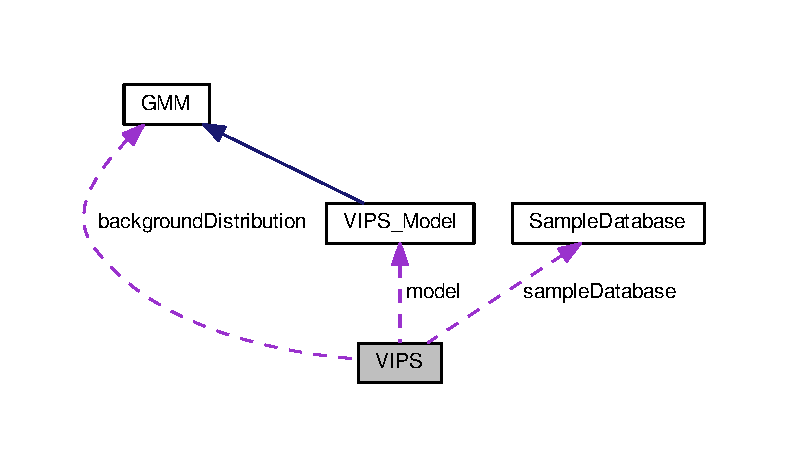
\includegraphics[width=350pt]{classVIPS__coll__graph}
\end{center}
\end{figure}
\subsection*{Public Member Functions}
\begin{DoxyCompactItemize}
\item 
\hyperlink{classVIPS_a468c5d01f08c35ca0243f02fe6cafeaf}{V\+I\+PS} (int num\+\_\+dimensions, int num\+\_\+threads)
\item 
void \hyperlink{classVIPS_aba18c184ad6826ac8458fb573af7bcbc}{delete\+\_\+low\+\_\+weight\+\_\+components} (double min\+\_\+weight)
\item 
void \hyperlink{classVIPS_adff46a3464207e55c4e699e6d869d40f}{add\+\_\+samples\+\_\+to\+\_\+database} (arma\+::mat new\+\_\+samples, arma\+::vec new\+\_\+target\+\_\+densities, arma\+::uvec used\+\_\+components)
\item 
void \hyperlink{classVIPS_a8e90dcdcf50ffca10fbb9dbfd8176e22}{recompute\+\_\+densities} (bool update\+\_\+log\+\_\+densities\+\_\+on\+\_\+model\+\_\+comps=true, bool update\+\_\+log\+\_\+densities\+\_\+on\+\_\+background\+\_\+dist=true)
\item 
void \hyperlink{classVIPS_a2f862569f67b4061bbcd267108adede9}{activate\+\_\+newest\+\_\+samples} (int N)
\item 
void \hyperlink{classVIPS_a6e88b8a4ffd410ee100455458b5d9e3b}{update\+\_\+targets\+\_\+for\+\_\+\+K\+L\+\_\+bounds} (bool update\+\_\+weight\+\_\+targets, bool update\+\_\+comp\+\_\+targets)
\item 
void \hyperlink{classVIPS_afda46fdd2494774ae418a9fcccda905f}{promote\+\_\+samples\+\_\+to\+\_\+components} (int N, double max\+\_\+exploration\+\_\+bonus, double tau, bool only\+\_\+check\+\_\+active\+\_\+samples, int max\+\_\+samples)
\item 
std\+::tuple$<$ double, vec, vec $>$ \hyperlink{classVIPS_aebb5f603c3ec270f625eb2bd4d3efe3a}{update\+\_\+weights} (double epsilon, double tau, double entropy\+\_\+bound)
\item 
arma\+::vec \hyperlink{classVIPS_aac85e9be0da81e9fa603528aa7958a0a}{adapt\+\_\+\+K\+L\+\_\+bound\+\_\+for\+\_\+comp\+\_\+update} (double max\+\_\+kl\+\_\+bound, double factor)
\item 
arma\+::vec \hyperlink{classVIPS_a84a2917e689f48562e0f951a8f577723}{update\+\_\+components} (double max\+\_\+kl\+\_\+bound, double factor, double tau, double ridge\+\_\+coefficient, vec entropy\+\_\+bounds, double max\+\_\+active\+\_\+samples, bool dont\+\_\+learn\+\_\+correlations)
\item 
void \hyperlink{classVIPS_aeb4149a37ec733f22ef9e302439c42da}{add\+\_\+components} (arma\+::vec new\+\_\+weights\+\_\+total, arma\+::mat new\+\_\+means, arma\+::cube new\+\_\+covs)
\item 
double \hyperlink{classVIPS_acfc4f6911881e21b1b06276f7514bcfa}{get\+\_\+entropy\+\_\+estimate\+\_\+on\+\_\+active\+\_\+samples} ()
\item 
double \hyperlink{classVIPS_aeec7ba6219e433ad9ab6214e4ed0dd4a}{get\+\_\+entropy\+\_\+estimate\+\_\+on\+\_\+gmm\+\_\+samples} (int num\+\_\+samples=10000)
\item 
std\+::tuple$<$ arma\+::mat, arma\+::vec, arma\+::mat, arma\+::mat, arma\+::vec, arma\+::mat, arma\+::mat, arma\+::mat, arma\+::mat $>$ \hyperlink{classVIPS_ac824a4180e5a8475eeb5a7c68a6483b6}{get\+\_\+debug\+\_\+info} ()
\item 
int {\bfseries get\+Num\+Samples} ()\hypertarget{classVIPS_a9c3c1617a3e8be6b02a7b5166711bb46}{}\label{classVIPS_a9c3c1617a3e8be6b02a7b5166711bb46}

\end{DoxyCompactItemize}
\subsection*{Public Attributes}
\begin{DoxyCompactItemize}
\item 
\hyperlink{classVIPS__Model}{V\+I\+P\+S\+\_\+\+Model} {\bfseries model}\hypertarget{classVIPS_a9929f2b77be4949c57ac9008d5f3ec5c}{}\label{classVIPS_a9929f2b77be4949c57ac9008d5f3ec5c}

\item 
\hyperlink{classGMM}{G\+MM} {\bfseries background\+Distribution}\hypertarget{classVIPS_a9e9d133d270287a47e693ebda4199a91}{}\label{classVIPS_a9e9d133d270287a47e693ebda4199a91}

\item 
\hyperlink{classSampleDatabase}{Sample\+Database} {\bfseries sample\+Database}\hypertarget{classVIPS_a29ce35cb0e4ba5bbff626bcccd88417b}{}\label{classVIPS_a29ce35cb0e4ba5bbff626bcccd88417b}

\end{DoxyCompactItemize}
\subsection*{Protected Attributes}
\begin{DoxyCompactItemize}
\item 
int {\bfseries num\+\_\+threads}\hypertarget{classVIPS_accccca2a57a73de29ee07a8a76c9c941}{}\label{classVIPS_accccca2a57a73de29ee07a8a76c9c941}

\item 
int {\bfseries num\+\_\+dimensions}\hypertarget{classVIPS_ae2fc04069049b703933aa1a1834067a2}{}\label{classVIPS_ae2fc04069049b703933aa1a1834067a2}

\item 
int {\bfseries num\+\_\+samples}\hypertarget{classVIPS_ac99a855e6f284c3028435dd23fea3c06}{}\label{classVIPS_ac99a855e6f284c3028435dd23fea3c06}

\item 
arma\+::mat {\bfseries samples}\hypertarget{classVIPS_a16a3f01a04f8a2aabb4972912e4f105d}{}\label{classVIPS_a16a3f01a04f8a2aabb4972912e4f105d}

\item 
arma\+::vec {\bfseries target\+\_\+densities}\hypertarget{classVIPS_a27193a3430c50755c6342ed370df794b}{}\label{classVIPS_a27193a3430c50755c6342ed370df794b}

\item 
arma\+::mat {\bfseries log\+\_\+densities\+\_\+on\+\_\+model\+\_\+comps}\hypertarget{classVIPS_acd32741f14cf0d1793cf6e64b636fcc0}{}\label{classVIPS_acd32741f14cf0d1793cf6e64b636fcc0}

\item 
arma\+::mat {\bfseries log\+\_\+joint\+\_\+densities}\hypertarget{classVIPS_a4a84ac52b3f3475ad4efeabc6d92c1c3}{}\label{classVIPS_a4a84ac52b3f3475ad4efeabc6d92c1c3}

\item 
arma\+::vec {\bfseries log\+\_\+densities\+\_\+on\+\_\+model}\hypertarget{classVIPS_a6c98147f1bba2bf4467714bb1070f5b6}{}\label{classVIPS_a6c98147f1bba2bf4467714bb1070f5b6}

\item 
arma\+::mat {\bfseries log\+\_\+responsibilities}\hypertarget{classVIPS_a17f93d9215dbee5127d94fd65b61848e}{}\label{classVIPS_a17f93d9215dbee5127d94fd65b61848e}

\item 
arma\+::mat {\bfseries log\+\_\+densities\+\_\+on\+\_\+background\+\_\+dist}\hypertarget{classVIPS_abe994fe945632006165a985c4c89f4b8}{}\label{classVIPS_abe994fe945632006165a985c4c89f4b8}

\item 
arma\+::rowvec {\bfseries offsets\+\_\+for\+\_\+model\+\_\+joint\+\_\+densities}\hypertarget{classVIPS_a05cf1526a1aaa34cfd76f2f7b9f1f653}{}\label{classVIPS_a05cf1526a1aaa34cfd76f2f7b9f1f653}

\item 
arma\+::rowvec {\bfseries sum\+\_\+of\+\_\+joint\+\_\+densities\+\_\+with\+\_\+offsets}\hypertarget{classVIPS_a825e8ea57d1c72d0941e1d5fc4c68ab3}{}\label{classVIPS_a825e8ea57d1c72d0941e1d5fc4c68ab3}

\item 
arma\+::mat {\bfseries importance\+\_\+weights}\hypertarget{classVIPS_ac318b08a7f1e3e7d386da8921f69db5c}{}\label{classVIPS_ac318b08a7f1e3e7d386da8921f69db5c}

\item 
arma\+::mat {\bfseries importance\+\_\+weights\+\_\+normalized}\hypertarget{classVIPS_aedb1fb27412374a577219711f083dd7d}{}\label{classVIPS_aedb1fb27412374a577219711f083dd7d}

\end{DoxyCompactItemize}


\subsection{Constructor \& Destructor Documentation}
\index{V\+I\+PS@{V\+I\+PS}!V\+I\+PS@{V\+I\+PS}}
\index{V\+I\+PS@{V\+I\+PS}!V\+I\+PS@{V\+I\+PS}}
\subsubsection[{\texorpdfstring{V\+I\+P\+S(int num\+\_\+dimensions, int num\+\_\+threads)}{VIPS(int num_dimensions, int num_threads)}}]{\setlength{\rightskip}{0pt plus 5cm}V\+I\+P\+S\+::\+V\+I\+PS (
\begin{DoxyParamCaption}
\item[{int}]{num\+\_\+dimensions, }
\item[{int}]{num\+\_\+threads}
\end{DoxyParamCaption}
)}\hypertarget{classVIPS_a468c5d01f08c35ca0243f02fe6cafeaf}{}\label{classVIPS_a468c5d01f08c35ca0243f02fe6cafeaf}
Main class implementing the Learn-\/\+To-\/\+Sample algorithm 
\begin{DoxyParams}{Parameters}
{\em num\+\_\+dimensions} & -\/ dimensionality of the sampling problem \\
\hline
{\em num\+\_\+threads} & -\/ number of threads to use \\
\hline
\end{DoxyParams}


\subsection{Member Function Documentation}
\index{V\+I\+PS@{V\+I\+PS}!activate\+\_\+newest\+\_\+samples@{activate\+\_\+newest\+\_\+samples}}
\index{activate\+\_\+newest\+\_\+samples@{activate\+\_\+newest\+\_\+samples}!V\+I\+PS@{V\+I\+PS}}
\subsubsection[{\texorpdfstring{activate\+\_\+newest\+\_\+samples(int N)}{activate_newest_samples(int N)}}]{\setlength{\rightskip}{0pt plus 5cm}void V\+I\+P\+S\+::activate\+\_\+newest\+\_\+samples (
\begin{DoxyParamCaption}
\item[{int}]{N}
\end{DoxyParamCaption}
)}\hypertarget{classVIPS_a2f862569f67b4061bbcd267108adede9}{}\label{classVIPS_a2f862569f67b4061bbcd267108adede9}
Selects the N most recent samples and activates them (i.\+e. uses them for the upcoming learning iteration).~\newline
 Makes sure, that all relevant data (e.\+g. densities, importance weights, etc.) gets updated 
\begin{DoxyParams}{Parameters}
{\em N} & -\/ the maximum number of recent samples to be activated, actually number of activated samples might be less, iff the sample database does not contain sufficient samples. \\
\hline
\end{DoxyParams}
\index{V\+I\+PS@{V\+I\+PS}!adapt\+\_\+\+K\+L\+\_\+bound\+\_\+for\+\_\+comp\+\_\+update@{adapt\+\_\+\+K\+L\+\_\+bound\+\_\+for\+\_\+comp\+\_\+update}}
\index{adapt\+\_\+\+K\+L\+\_\+bound\+\_\+for\+\_\+comp\+\_\+update@{adapt\+\_\+\+K\+L\+\_\+bound\+\_\+for\+\_\+comp\+\_\+update}!V\+I\+PS@{V\+I\+PS}}
\subsubsection[{\texorpdfstring{adapt\+\_\+\+K\+L\+\_\+bound\+\_\+for\+\_\+comp\+\_\+update(double max\+\_\+kl\+\_\+bound, double factor)}{adapt_KL_bound_for_comp_update(double max_kl_bound, double factor)}}]{\setlength{\rightskip}{0pt plus 5cm}vec V\+I\+P\+S\+::adapt\+\_\+\+K\+L\+\_\+bound\+\_\+for\+\_\+comp\+\_\+update (
\begin{DoxyParamCaption}
\item[{double}]{max\+\_\+kl\+\_\+bound, }
\item[{double}]{factor}
\end{DoxyParamCaption}
)}\hypertarget{classVIPS_aac85e9be0da81e9fa603528aa7958a0a}{}\label{classVIPS_aac85e9be0da81e9fa603528aa7958a0a}
Adapts the KL bound based on the number of effective samples.~\newline
 The KL bound for each component is set to min(max\+\_\+kl\+\_\+bound, factor $\ast$ num\+\_\+eff\+\_\+samples(o)) 
\begin{DoxyParams}{Parameters}
{\em max\+\_\+kl\+\_\+bound} & -\/ hard upper bound for KL \\
\hline
{\em factor} & -\/ factor for computing the KL bound based on the number of effective samples \\
\hline
\end{DoxyParams}
\index{V\+I\+PS@{V\+I\+PS}!add\+\_\+components@{add\+\_\+components}}
\index{add\+\_\+components@{add\+\_\+components}!V\+I\+PS@{V\+I\+PS}}
\subsubsection[{\texorpdfstring{add\+\_\+components(arma\+::vec new\+\_\+weights\+\_\+total, arma\+::mat new\+\_\+means, arma\+::cube new\+\_\+covs)}{add_components(arma::vec new_weights_total, arma::mat new_means, arma::cube new_covs)}}]{\setlength{\rightskip}{0pt plus 5cm}void V\+I\+P\+S\+::add\+\_\+components (
\begin{DoxyParamCaption}
\item[{arma\+::vec}]{new\+\_\+weights\+\_\+total, }
\item[{arma\+::mat}]{new\+\_\+means, }
\item[{arma\+::cube}]{new\+\_\+covs}
\end{DoxyParamCaption}
)}\hypertarget{classVIPS_aeb4149a37ec733f22ef9e302439c42da}{}\label{classVIPS_aeb4149a37ec733f22ef9e302439c42da}
Adds new components. 
\begin{DoxyParams}{Parameters}
{\em new\+\_\+weights\+\_\+total} & -\/ new weights of the \hyperlink{classGMM}{G\+MM} (including existing components) \\
\hline
{\em new\+\_\+means} & -\/ matrix of size N\+\_\+dimensions x N\+\_\+new\+Components specifying the means of the new components \\
\hline
{\em new\+\_\+covs} & -\/ cube of size N\+\_\+dimensions x N\+\_\+dimensions x N\+\_\+new\+Components specifying the covariance matrices of the new components \\
\hline
\end{DoxyParams}
\index{V\+I\+PS@{V\+I\+PS}!add\+\_\+samples\+\_\+to\+\_\+database@{add\+\_\+samples\+\_\+to\+\_\+database}}
\index{add\+\_\+samples\+\_\+to\+\_\+database@{add\+\_\+samples\+\_\+to\+\_\+database}!V\+I\+PS@{V\+I\+PS}}
\subsubsection[{\texorpdfstring{add\+\_\+samples\+\_\+to\+\_\+database(arma\+::mat new\+\_\+samples, arma\+::vec new\+\_\+target\+\_\+densities, arma\+::uvec used\+\_\+components)}{add_samples_to_database(arma::mat new_samples, arma::vec new_target_densities, arma::uvec used_components)}}]{\setlength{\rightskip}{0pt plus 5cm}void V\+I\+P\+S\+::add\+\_\+samples\+\_\+to\+\_\+database (
\begin{DoxyParamCaption}
\item[{arma\+::mat}]{new\+\_\+samples, }
\item[{arma\+::vec}]{new\+\_\+target\+\_\+densities, }
\item[{arma\+::uvec}]{used\+\_\+components}
\end{DoxyParamCaption}
)}\hypertarget{classVIPS_adff46a3464207e55c4e699e6d869d40f}{}\label{classVIPS_adff46a3464207e55c4e699e6d869d40f}
Adds new samples to the database. Note that the samples will not be used for learning, until they have been activated (see activate\+\_\+newest\+\_\+samples).~\newline
 The samples are assumed to have been drawn from the current model and the indices of the relevant components are to be provided for computing background distributions when necessary. 
\begin{DoxyParams}{Parameters}
{\em new\+\_\+samples} & -\/ a matrix of size N\+\_\+dimensions X N\+\_\+samples \\
\hline
{\em new\+\_\+target\+\_\+densities} & -\/ a vector of size N\+\_\+samples containing the unnormalized densities on the target distribution \\
\hline
{\em used\+\_\+components} & -\/ a vector of size N\+\_\+samples containing the indices of the components the corresponding samples have been drawn from \\
\hline
\end{DoxyParams}
\begin{DoxySeeAlso}{See also}
\hyperlink{classVIPS_a2f862569f67b4061bbcd267108adede9}{activate\+\_\+newest\+\_\+samples} 
\end{DoxySeeAlso}
\index{V\+I\+PS@{V\+I\+PS}!delete\+\_\+low\+\_\+weight\+\_\+components@{delete\+\_\+low\+\_\+weight\+\_\+components}}
\index{delete\+\_\+low\+\_\+weight\+\_\+components@{delete\+\_\+low\+\_\+weight\+\_\+components}!V\+I\+PS@{V\+I\+PS}}
\subsubsection[{\texorpdfstring{delete\+\_\+low\+\_\+weight\+\_\+components(double min\+\_\+weight)}{delete_low_weight_components(double min_weight)}}]{\setlength{\rightskip}{0pt plus 5cm}void V\+I\+P\+S\+::delete\+\_\+low\+\_\+weight\+\_\+components (
\begin{DoxyParamCaption}
\item[{double}]{min\+\_\+weight}
\end{DoxyParamCaption}
)}\hypertarget{classVIPS_aba18c184ad6826ac8458fb573af7bcbc}{}\label{classVIPS_aba18c184ad6826ac8458fb573af7bcbc}
Removes all components with weight below the given threshold, and renormalized the weights afterwards 
\begin{DoxyParams}{Parameters}
{\em min\+\_\+weight} & -\/ threshold for keeping components \\
\hline
\end{DoxyParams}
\index{V\+I\+PS@{V\+I\+PS}!get\+\_\+debug\+\_\+info@{get\+\_\+debug\+\_\+info}}
\index{get\+\_\+debug\+\_\+info@{get\+\_\+debug\+\_\+info}!V\+I\+PS@{V\+I\+PS}}
\subsubsection[{\texorpdfstring{get\+\_\+debug\+\_\+info()}{get_debug_info()}}]{\setlength{\rightskip}{0pt plus 5cm}std\+::tuple$<$ mat, vec, mat, mat, vec, mat, mat, mat, mat $>$ V\+I\+P\+S\+::get\+\_\+debug\+\_\+info (
\begin{DoxyParamCaption}
{}
\end{DoxyParamCaption}
)}\hypertarget{classVIPS_ac824a4180e5a8475eeb5a7c68a6483b6}{}\label{classVIPS_ac824a4180e5a8475eeb5a7c68a6483b6}
Get various densities, importance weights, etc. for debug purposes. \begin{DoxyReturn}{Returns}
a tuple, st. ~\newline
 tuple\mbox{[}0\mbox{]} contains the samples ~\newline
 tuple\mbox{[}1\mbox{]} contains the unnormalized target densities ~\newline
 tuple\mbox{[}2\mbox{]} contains the log densities on each model p(s$\vert$o) ~\newline
 tuple\mbox{[}3\mbox{]} contains the joint log densities p(s,o) ~\newline
 tuple\mbox{[}4\mbox{]} contains the \hyperlink{classGMM}{G\+MM} densities p(s) ~\newline
 tuple\mbox{[}5\mbox{]} contains the log responsibilities p(o$\vert$s) ~\newline
 tuple\mbox{[}6\mbox{]} contains the densitis on the background distribution q(s) ~\newline
 tuple\mbox{[}7\mbox{]} contains the importance weights ~\newline
 tuple\mbox{[}8\mbox{]} contains the normalized importance weights 
\end{DoxyReturn}
\index{V\+I\+PS@{V\+I\+PS}!get\+\_\+entropy\+\_\+estimate\+\_\+on\+\_\+active\+\_\+samples@{get\+\_\+entropy\+\_\+estimate\+\_\+on\+\_\+active\+\_\+samples}}
\index{get\+\_\+entropy\+\_\+estimate\+\_\+on\+\_\+active\+\_\+samples@{get\+\_\+entropy\+\_\+estimate\+\_\+on\+\_\+active\+\_\+samples}!V\+I\+PS@{V\+I\+PS}}
\subsubsection[{\texorpdfstring{get\+\_\+entropy\+\_\+estimate\+\_\+on\+\_\+active\+\_\+samples()}{get_entropy_estimate_on_active_samples()}}]{\setlength{\rightskip}{0pt plus 5cm}double V\+I\+P\+S\+::get\+\_\+entropy\+\_\+estimate\+\_\+on\+\_\+active\+\_\+samples (
\begin{DoxyParamCaption}
{}
\end{DoxyParamCaption}
)}\hypertarget{classVIPS_acfc4f6911881e21b1b06276f7514bcfa}{}\label{classVIPS_acfc4f6911881e21b1b06276f7514bcfa}
Returns a (weighted importance sampling) Monte-\/\+Carlo estimate of the entropy of the learned model. The entropy is computed based on the active samples. As this entropy is computed based on precomputed values \mbox{[}importance weights and log(p(x))\mbox{]} th evaluation is very fast. However, if the number of active samples is still low or the samples are not \char`\"{}fresh\char`\"{} (low importance weights), the estimate can be quite bad. see \hyperlink{classVIPS_aeec7ba6219e433ad9ab6214e4ed0dd4a}{get\+\_\+entropy\+\_\+estimate\+\_\+on\+\_\+gmm\+\_\+samples()} for a slower, but usually more accurate estimate. \begin{DoxyReturn}{Returns}
a Monte-\/\+Carlo estimate of the entropy of the learned Gaussian Mixture Model 
\end{DoxyReturn}
\begin{DoxySeeAlso}{See also}
\hyperlink{classVIPS_aeec7ba6219e433ad9ab6214e4ed0dd4a}{get\+\_\+entropy\+\_\+estimate\+\_\+on\+\_\+gmm\+\_\+samples()} 
\end{DoxySeeAlso}
\index{V\+I\+PS@{V\+I\+PS}!get\+\_\+entropy\+\_\+estimate\+\_\+on\+\_\+gmm\+\_\+samples@{get\+\_\+entropy\+\_\+estimate\+\_\+on\+\_\+gmm\+\_\+samples}}
\index{get\+\_\+entropy\+\_\+estimate\+\_\+on\+\_\+gmm\+\_\+samples@{get\+\_\+entropy\+\_\+estimate\+\_\+on\+\_\+gmm\+\_\+samples}!V\+I\+PS@{V\+I\+PS}}
\subsubsection[{\texorpdfstring{get\+\_\+entropy\+\_\+estimate\+\_\+on\+\_\+gmm\+\_\+samples(int num\+\_\+samples=10000)}{get_entropy_estimate_on_gmm_samples(int num_samples=10000)}}]{\setlength{\rightskip}{0pt plus 5cm}double V\+I\+P\+S\+::get\+\_\+entropy\+\_\+estimate\+\_\+on\+\_\+gmm\+\_\+samples (
\begin{DoxyParamCaption}
\item[{int}]{N = {\ttfamily 10000}}
\end{DoxyParamCaption}
)}\hypertarget{classVIPS_aeec7ba6219e433ad9ab6214e4ed0dd4a}{}\label{classVIPS_aeec7ba6219e433ad9ab6214e4ed0dd4a}
Returns a Monte-\/\+Carlo estimate of the entropy of the learned model. This methods draws new samples from the learned model and evaluated their log-\/densities log(p(x)). The entropy of the learned model is then approximated as H(p)  -\/1/N  log(p(x)). see \hyperlink{classVIPS_acfc4f6911881e21b1b06276f7514bcfa}{get\+\_\+entropy\+\_\+estimate\+\_\+on\+\_\+active\+\_\+samples()} for a faster, but usually less accurate estimate. 
\begin{DoxyParams}{Parameters}
{\em N} & -\/ the number of samples that should be drawn for computing the estimate \\
\hline
\end{DoxyParams}
\begin{DoxyReturn}{Returns}
a Monte-\/\+Carlo estimate of the entropy of the learned Gaussian Mixture Model 
\end{DoxyReturn}
\begin{DoxySeeAlso}{See also}
\hyperlink{classVIPS_acfc4f6911881e21b1b06276f7514bcfa}{get\+\_\+entropy\+\_\+estimate\+\_\+on\+\_\+active\+\_\+samples()} 
\end{DoxySeeAlso}
\index{V\+I\+PS@{V\+I\+PS}!promote\+\_\+samples\+\_\+to\+\_\+components@{promote\+\_\+samples\+\_\+to\+\_\+components}}
\index{promote\+\_\+samples\+\_\+to\+\_\+components@{promote\+\_\+samples\+\_\+to\+\_\+components}!V\+I\+PS@{V\+I\+PS}}
\subsubsection[{\texorpdfstring{promote\+\_\+samples\+\_\+to\+\_\+components(int N, double max\+\_\+exploration\+\_\+bonus, double tau, bool only\+\_\+check\+\_\+active\+\_\+samples, int max\+\_\+samples)}{promote_samples_to_components(int N, double max_exploration_bonus, double tau, bool only_check_active_samples, int max_samples)}}]{\setlength{\rightskip}{0pt plus 5cm}void V\+I\+P\+S\+::promote\+\_\+samples\+\_\+to\+\_\+components (
\begin{DoxyParamCaption}
\item[{int}]{N, }
\item[{double}]{max\+\_\+exploration\+\_\+bonus, }
\item[{double}]{tau, }
\item[{bool}]{only\+\_\+check\+\_\+active\+\_\+samples, }
\item[{int}]{max\+\_\+samples}
\end{DoxyParamCaption}
)}\hypertarget{classVIPS_afda46fdd2494774ae418a9fcccda905f}{}\label{classVIPS_afda46fdd2494774ae418a9fcccda905f}
Selects promising locations among the current samples and create new components at these positions. The covariance matrices are given by the weighted sums of the covariance matrices current model, where the weights are given by the responsibilities of the model components for the new location. Locations are promising if the residual given by residual = log(p\+\_\+intractable(x)) -\/ log(p\+\_\+model(x) + exp(max\+\_\+exploration\+\_\+bonus)) is high.


\begin{DoxyParams}{Parameters}
{\em N} & -\/ the number of samples to be promoted \\
\hline
{\em max\+\_\+exploration\+\_\+bonus} & -\/ maximum bonus for samples that have low density on the current model \\
\hline
{\em only\+\_\+check\+\_\+active\+\_\+samples} & -\/ if set to true, the residual is computed on the active samples only, otherwise, the resiudal is computed for all samples in the sample database. \\
\hline
{\em max\+\_\+samples} & -\/ maximum number of samples to be considered \\
\hline
\end{DoxyParams}
\index{V\+I\+PS@{V\+I\+PS}!recompute\+\_\+densities@{recompute\+\_\+densities}}
\index{recompute\+\_\+densities@{recompute\+\_\+densities}!V\+I\+PS@{V\+I\+PS}}
\subsubsection[{\texorpdfstring{recompute\+\_\+densities(bool update\+\_\+log\+\_\+densities\+\_\+on\+\_\+model\+\_\+comps=true, bool update\+\_\+log\+\_\+densities\+\_\+on\+\_\+background\+\_\+dist=true)}{recompute_densities(bool update_log_densities_on_model_comps=true, bool update_log_densities_on_background_dist=true)}}]{\setlength{\rightskip}{0pt plus 5cm}void V\+I\+P\+S\+::recompute\+\_\+densities (
\begin{DoxyParamCaption}
\item[{bool}]{update\+\_\+log\+\_\+densities\+\_\+on\+\_\+model\+\_\+comps = {\ttfamily true}, }
\item[{bool}]{update\+\_\+log\+\_\+densities\+\_\+on\+\_\+background\+\_\+dist = {\ttfamily true}}
\end{DoxyParamCaption}
)}\hypertarget{classVIPS_a8e90dcdcf50ffca10fbb9dbfd8176e22}{}\label{classVIPS_a8e90dcdcf50ffca10fbb9dbfd8176e22}
Recomputes the densities of various distributions as well as the importance weights.~\newline
 Manual invocation is in general not necessary, as the densities are automatic updated, e.\+g. after weight changes, component changes, adding components, etc. 
\begin{DoxyParams}{Parameters}
{\em update\+\_\+log\+\_\+densities\+\_\+on\+\_\+model\+\_\+comps} & -\/ if this flag is set to false, assume that the density-\/evaluations for each \hyperlink{classGMM}{G\+MM} component is up-\/to-\/date, e.\+g. because only the \hyperlink{classGMM}{G\+MM} weights have changed \\
\hline
{\em update\+\_\+log\+\_\+densities\+\_\+on\+\_\+model\+\_\+background\+\_\+dist} & -\/ if this flag is set to false, assume that the density evaluations for the background distribution are up-\/to-\/date, e.\+g. because it was not changed at all \\
\hline
\end{DoxyParams}
\index{V\+I\+PS@{V\+I\+PS}!update\+\_\+components@{update\+\_\+components}}
\index{update\+\_\+components@{update\+\_\+components}!V\+I\+PS@{V\+I\+PS}}
\subsubsection[{\texorpdfstring{update\+\_\+components(double max\+\_\+kl\+\_\+bound, double factor, double tau, double ridge\+\_\+coefficient, vec entropy\+\_\+bounds, double max\+\_\+active\+\_\+samples, bool dont\+\_\+learn\+\_\+correlations)}{update_components(double max_kl_bound, double factor, double tau, double ridge_coefficient, vec entropy_bounds, double max_active_samples, bool dont_learn_correlations)}}]{\setlength{\rightskip}{0pt plus 5cm}vec V\+I\+P\+S\+::update\+\_\+components (
\begin{DoxyParamCaption}
\item[{double}]{max\+\_\+kl\+\_\+bound, }
\item[{double}]{factor, }
\item[{double}]{tau, }
\item[{double}]{ridge\+\_\+coefficient, }
\item[{vec}]{entropy\+\_\+bounds, }
\item[{double}]{max\+\_\+active\+\_\+samples, }
\item[{bool}]{dont\+\_\+learn\+\_\+correlations}
\end{DoxyParamCaption}
)}\hypertarget{classVIPS_a84a2917e689f48562e0f951a8f577723}{}\label{classVIPS_a84a2917e689f48562e0f951a8f577723}
Updates the components p(s$\vert$o). 
\begin{DoxyParams}{Parameters}
{\em max\+\_\+kl\+\_\+bound} & -\/ hard upper bound for each KL bound \\
\hline
{\em factor} & -\/ factor for computing the KL bound for each component based on its number of effective samples \\
\hline
{\em tau} & -\/ entropy coefficient \\
\hline
{\em ridge\+\_\+coefficient} & -\/ coefficient used for regularization when fitting the quadratic surrogate \\
\hline
{\em entropy\+\_\+bounds} & -\/ lower bound on entropy \\
\hline
{\em max\+\_\+active\+\_\+samples} & -\/ size of the subset of samples that should be used for each component update \\
\hline
{\em dont\+\_\+learn\+\_\+correlations} & -\/ iff true, fit a quadratic surrogate where R is diagonal (experimental) \\
\hline
\end{DoxyParams}
\index{V\+I\+PS@{V\+I\+PS}!update\+\_\+targets\+\_\+for\+\_\+\+K\+L\+\_\+bounds@{update\+\_\+targets\+\_\+for\+\_\+\+K\+L\+\_\+bounds}}
\index{update\+\_\+targets\+\_\+for\+\_\+\+K\+L\+\_\+bounds@{update\+\_\+targets\+\_\+for\+\_\+\+K\+L\+\_\+bounds}!V\+I\+PS@{V\+I\+PS}}
\subsubsection[{\texorpdfstring{update\+\_\+targets\+\_\+for\+\_\+\+K\+L\+\_\+bounds(bool update\+\_\+weight\+\_\+targets, bool update\+\_\+comp\+\_\+targets)}{update_targets_for_KL_bounds(bool update_weight_targets, bool update_comp_targets)}}]{\setlength{\rightskip}{0pt plus 5cm}void V\+I\+P\+S\+::update\+\_\+targets\+\_\+for\+\_\+\+K\+L\+\_\+bounds (
\begin{DoxyParamCaption}
\item[{bool}]{update\+\_\+weight\+\_\+targets, }
\item[{bool}]{update\+\_\+comp\+\_\+targets}
\end{DoxyParamCaption}
)}\hypertarget{classVIPS_a6e88b8a4ffd410ee100455458b5d9e3b}{}\label{classVIPS_a6e88b8a4ffd410ee100455458b5d9e3b}
Sets the current components p(s$\vert$o) and the current weight distribution p(o) as the target for the respective KL bounds. 
\begin{DoxyParams}{Parameters}
{\em update\+\_\+weight\+\_\+targets} & -\/ only update the weight targets if this is set to true \\
\hline
{\em update\+\_\+comp\+\_\+targets} & -\/ only update the component targets if this ist set to true \\
\hline
\end{DoxyParams}
\index{V\+I\+PS@{V\+I\+PS}!update\+\_\+weights@{update\+\_\+weights}}
\index{update\+\_\+weights@{update\+\_\+weights}!V\+I\+PS@{V\+I\+PS}}
\subsubsection[{\texorpdfstring{update\+\_\+weights(double epsilon, double tau, double entropy\+\_\+bound)}{update_weights(double epsilon, double tau, double entropy_bound)}}]{\setlength{\rightskip}{0pt plus 5cm}std\+::tuple$<$ double, vec, vec $>$ V\+I\+P\+S\+::update\+\_\+weights (
\begin{DoxyParamCaption}
\item[{double}]{epsilon, }
\item[{double}]{tau, }
\item[{double}]{entropy\+\_\+bound}
\end{DoxyParamCaption}
)}\hypertarget{classVIPS_aebb5f603c3ec270f625eb2bd4d3efe3a}{}\label{classVIPS_aebb5f603c3ec270f625eb2bd4d3efe3a}
update the component weights p(o). 
\begin{DoxyParams}{Parameters}
{\em epsilon} & is the KL bound \\
\hline
{\em tau} & is the entropy coefficient \\
\hline
\end{DoxyParams}
\begin{DoxyReturn}{Returns}
a tuple, s.\+t. tuple\mbox{[}0\mbox{]} contains the KL D(p\+\_\+new(o)$\vert$$\vert$p\+\_\+old(o)) tuple\mbox{[}1\mbox{]} contains the rewards for each component that was used during the optimization tuple\mbox{[}2\mbox{]} contains a sample-\/estimate of the expected, unnormalized log-\/densities of the desired distribution 
\end{DoxyReturn}


The documentation for this class was generated from the following files\+:\begin{DoxyCompactItemize}
\item 
V\+I\+P\+S.\+h\item 
V\+I\+P\+S.\+cpp\end{DoxyCompactItemize}

\hypertarget{classVIPS__Model}{}\section{V\+I\+P\+S\+\_\+\+Model Class Reference}
\label{classVIPS__Model}\index{V\+I\+P\+S\+\_\+\+Model@{V\+I\+P\+S\+\_\+\+Model}}


Inheritance diagram for V\+I\+P\+S\+\_\+\+Model\+:\nopagebreak
\begin{figure}[H]
\begin{center}
\leavevmode
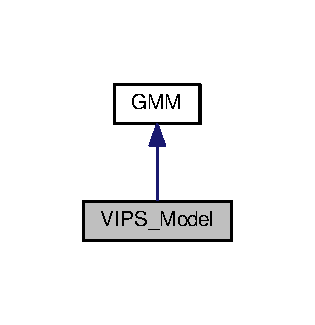
\includegraphics[width=151pt]{classVIPS__Model__inherit__graph}
\end{center}
\end{figure}


Collaboration diagram for V\+I\+P\+S\+\_\+\+Model\+:\nopagebreak
\begin{figure}[H]
\begin{center}
\leavevmode
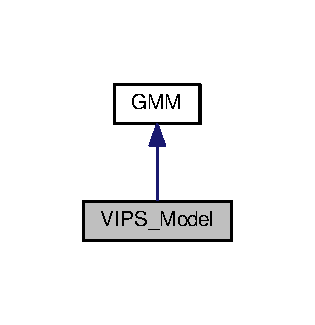
\includegraphics[width=151pt]{classVIPS__Model__coll__graph}
\end{center}
\end{figure}
\subsection*{Public Member Functions}
\begin{DoxyCompactItemize}
\item 
\hyperlink{classVIPS__Model_a7a17f89802a4e8be6ffefb92e691b602}{V\+I\+P\+S\+\_\+\+Model} (int dim, double initial\+\_\+kl\+\_\+bound=0.\+5)
\item 
void \hyperlink{classVIPS__Model_afcc9485205fd0c61801546703bffa5eb}{add\+\_\+components} (arma\+::mat new\+\_\+means, arma\+::cube new\+\_\+covs) override
\item 
void \hyperlink{classVIPS__Model_ab83e56934a07a6381e0cb4f9beab26fd}{add\+\_\+components\+\_\+inv\+Chols} (arma\+::mat new\+\_\+means, arma\+::cube new\+\_\+inv\+Chols) override
\item 
void \hyperlink{classVIPS__Model_a6b0edde4a9a744639e1588cff6a5fa23}{delete\+\_\+component} (int index) override
\item 
uvec \hyperlink{classVIPS__Model_a6c65151f76ac7e9f5bbc79288b30986b}{delete\+\_\+low\+\_\+weight\+\_\+components} (double min\+\_\+weight, int n\+\_\+del=300)
\item 
void \hyperlink{classVIPS__Model_acf045c351edff854a5f520beb2723832}{update\+\_\+histories} (vec expected\+\_\+target\+\_\+densities, vec component\+\_\+rewards, vec component\+\_\+weights)
\item 
void {\bfseries update\+\_\+num\+\_\+sample\+\_\+history} (uvec new\+\_\+samples)\hypertarget{classVIPS__Model_a72e9125d30c8ce56e9e6bb71fd01a00e}{}\label{classVIPS__Model_a72e9125d30c8ce56e9e6bb71fd01a00e}

\item 
std\+::tuple$<$ arma\+::cube, arma\+::cube, arma\+::mat, arma\+::vec, arma\+::vec $>$ \hyperlink{classVIPS__Model_a19bd5e5c123088de22c80df818f67994}{get\+Targets\+For\+K\+L\+Bounds} ()
\item 
void \hyperlink{classVIPS__Model_a6a99261a47556afce9b21c456000e44c}{update\+\_\+targets\+\_\+for\+\_\+\+K\+L\+\_\+bounds} (uvec component\+\_\+indices, bool update\+\_\+weight\+\_\+targets, bool update\+\_\+comp\+\_\+targets)
\item 
void \hyperlink{classVIPS__Model_ab4c62ebc6e2bc4c2bbefe65d95a66b00}{update\+\_\+targets\+\_\+for\+\_\+\+K\+L\+\_\+bounds} (bool update\+\_\+weight\+\_\+targets, bool update\+\_\+comp\+\_\+targets)
\item 
arma\+::vec {\bfseries get\+Last\+Etas\+For\+Comp\+Optimization} ()\hypertarget{classVIPS__Model_a8906614c09de390b4a9437cadd54218f}{}\label{classVIPS__Model_a8906614c09de390b4a9437cadd54218f}

\item 
void \hyperlink{classVIPS__Model_ac0f23dd73e953a9da2047075e6e3ff1c}{set\+Last\+Etas\+For\+Comp\+Optimization} (vec new\+\_\+last\+Etas)
\item 
arma\+::vec {\bfseries get\+Ridge\+Multipliers} ()\hypertarget{classVIPS__Model_a4a49a86c96c0f5239ed7b868e0de84b1}{}\label{classVIPS__Model_a4a49a86c96c0f5239ed7b868e0de84b1}

\item 
void \hyperlink{classVIPS__Model_a1d9d04bcc9b0dc392584804ac78f5813}{set\+Ridge\+Multipliers} (vec new\+\_\+ridge\+Multipliers)
\item 
arma\+::vec {\bfseries get\+Approx\+Reward\+Before\+Comp\+Update} ()\hypertarget{classVIPS__Model_a301ce5dc882e0ae70302a4712cc27fc1}{}\label{classVIPS__Model_a301ce5dc882e0ae70302a4712cc27fc1}

\item 
void \hyperlink{classVIPS__Model_a70c45c77ef2f4f7ebd5ddfe34c653da8}{set\+Approx\+Reward\+Before\+Comp\+Update} (vec new\+\_\+expected\+\_\+rewards)
\item 
arma\+::vec {\bfseries get\+K\+L\+Bounds} ()\hypertarget{classVIPS__Model_a24e9a1430fd5dd6d35db69c0490e65d7}{}\label{classVIPS__Model_a24e9a1430fd5dd6d35db69c0490e65d7}

\item 
void \hyperlink{classVIPS__Model_a5351e79e8fc43024659580eceaa89f56}{set\+K\+L\+Bounds} (vec new\+\_\+\+K\+L\+Bounds)
\end{DoxyCompactItemize}
\subsection*{Public Attributes}
\begin{DoxyCompactItemize}
\item 
arma\+::vec {\bfseries expected\+\_\+rewards}\hypertarget{classVIPS__Model_a3ab3746d8dd5832ea0bb0966224a4686}{}\label{classVIPS__Model_a3ab3746d8dd5832ea0bb0966224a4686}

\item 
arma\+::mat {\bfseries comp\+\_\+etd\+\_\+history}\hypertarget{classVIPS__Model_aae18271a9c94997444c4015ce24d666e}{}\label{classVIPS__Model_aae18271a9c94997444c4015ce24d666e}

\item 
arma\+::mat {\bfseries comp\+\_\+reward\+\_\+history}\hypertarget{classVIPS__Model_ad661b9d2f04bdc94a98e773144a8eb5d}{}\label{classVIPS__Model_ad661b9d2f04bdc94a98e773144a8eb5d}

\item 
arma\+::mat {\bfseries comp\+\_\+weight\+\_\+history}\hypertarget{classVIPS__Model_abbb57d44172beac50134b776f5308b0f}{}\label{classVIPS__Model_abbb57d44172beac50134b776f5308b0f}

\item 
arma\+::umat {\bfseries comp\+\_\+num\+\_\+samples\+\_\+history}\hypertarget{classVIPS__Model_a8ab784c4c6c4014a8255cb69813d7608}{}\label{classVIPS__Model_a8ab784c4c6c4014a8255cb69813d7608}

\end{DoxyCompactItemize}
\subsection*{Protected Member Functions}
\begin{DoxyCompactItemize}
\item 
void \hyperlink{classVIPS__Model_ad175bd3a39cec843b674a9d937c01654}{add\+\_\+meta\+\_\+info\+\_\+for\+\_\+components} (int N)
\end{DoxyCompactItemize}
\subsection*{Protected Attributes}
\begin{DoxyCompactItemize}
\item 
double {\bfseries initial\+\_\+kl\+\_\+bound}\hypertarget{classVIPS__Model_a9814472714c00939b479ddab4ed00fb2}{}\label{classVIPS__Model_a9814472714c00939b479ddab4ed00fb2}

\item 
arma\+::vec {\bfseries last\+\_\+etas\+\_\+for\+\_\+comp\+\_\+optimization}\hypertarget{classVIPS__Model_a0b2633c15ce1dee47eb88e1fba20de0c}{}\label{classVIPS__Model_a0b2633c15ce1dee47eb88e1fba20de0c}

\item 
arma\+::vec {\bfseries ridge\+\_\+multiplier}\hypertarget{classVIPS__Model_a15e0485d0b2d20cebe4aca4d106ac788}{}\label{classVIPS__Model_a15e0485d0b2d20cebe4aca4d106ac788}

\item 
arma\+::vec {\bfseries kl\+\_\+bounds}\hypertarget{classVIPS__Model_a0f298d2e9f9c0ea430c9785812dee158}{}\label{classVIPS__Model_a0f298d2e9f9c0ea430c9785812dee158}

\item 
arma\+::cube {\bfseries target\+\_\+inv\+\_\+chols}\hypertarget{classVIPS__Model_ac181de1cbdb425e501b43d61162577e0}{}\label{classVIPS__Model_ac181de1cbdb425e501b43d61162577e0}

\item 
arma\+::cube {\bfseries target\+\_\+chols}\hypertarget{classVIPS__Model_a79230bd91c1c0f986deb5357883ed2c0}{}\label{classVIPS__Model_a79230bd91c1c0f986deb5357883ed2c0}

\item 
arma\+::mat {\bfseries target\+\_\+means}\hypertarget{classVIPS__Model_a01e37d2f3d74b66b5f7e28c25e0f1b4c}{}\label{classVIPS__Model_a01e37d2f3d74b66b5f7e28c25e0f1b4c}

\item 
arma\+::vec {\bfseries target\+\_\+log\+\_\+weights}\hypertarget{classVIPS__Model_a6b16122ed1ffd5e18adb0e96bc1fd58b}{}\label{classVIPS__Model_a6b16122ed1ffd5e18adb0e96bc1fd58b}

\item 
arma\+::vec {\bfseries target\+\_\+weights}\hypertarget{classVIPS__Model_adce427fb02e181c2a90bb2b095f6edaf}{}\label{classVIPS__Model_adce427fb02e181c2a90bb2b095f6edaf}

\end{DoxyCompactItemize}


\subsection{Constructor \& Destructor Documentation}
\index{V\+I\+P\+S\+\_\+\+Model@{V\+I\+P\+S\+\_\+\+Model}!V\+I\+P\+S\+\_\+\+Model@{V\+I\+P\+S\+\_\+\+Model}}
\index{V\+I\+P\+S\+\_\+\+Model@{V\+I\+P\+S\+\_\+\+Model}!V\+I\+P\+S\+\_\+\+Model@{V\+I\+P\+S\+\_\+\+Model}}
\subsubsection[{\texorpdfstring{V\+I\+P\+S\+\_\+\+Model(int dim, double initial\+\_\+kl\+\_\+bound=0.\+5)}{VIPS_Model(int dim, double initial_kl_bound=0.5)}}]{\setlength{\rightskip}{0pt plus 5cm}V\+I\+P\+S\+\_\+\+Model\+::\+V\+I\+P\+S\+\_\+\+Model (
\begin{DoxyParamCaption}
\item[{int}]{dim, }
\item[{double}]{initial\+\_\+kl\+\_\+bound = {\ttfamily 0.5}}
\end{DoxyParamCaption}
)}\hypertarget{classVIPS__Model_a7a17f89802a4e8be6ffefb92e691b602}{}\label{classVIPS__Model_a7a17f89802a4e8be6ffefb92e691b602}
The G\+M\+M-\/model learned by \hyperlink{classVIPS}{V\+I\+PS}. This class extends \hyperlink{classGMM}{G\+MM} to include learning related meta information. 
\begin{DoxyParams}{Parameters}
{\em dim} & number of dimensions \\
\hline
{\em initial\+\_\+kl\+\_\+bound} & \\
\hline
\end{DoxyParams}


\subsection{Member Function Documentation}
\index{V\+I\+P\+S\+\_\+\+Model@{V\+I\+P\+S\+\_\+\+Model}!add\+\_\+components@{add\+\_\+components}}
\index{add\+\_\+components@{add\+\_\+components}!V\+I\+P\+S\+\_\+\+Model@{V\+I\+P\+S\+\_\+\+Model}}
\subsubsection[{\texorpdfstring{add\+\_\+components(arma\+::mat new\+\_\+means, arma\+::cube new\+\_\+covs) override}{add_components(arma::mat new_means, arma::cube new_covs) override}}]{\setlength{\rightskip}{0pt plus 5cm}void V\+I\+P\+S\+\_\+\+Model\+::add\+\_\+components (
\begin{DoxyParamCaption}
\item[{arma\+::mat}]{new\+\_\+means, }
\item[{arma\+::cube}]{new\+\_\+covs}
\end{DoxyParamCaption}
)\hspace{0.3cm}{\ttfamily [override]}}\hypertarget{classVIPS__Model_afcc9485205fd0c61801546703bffa5eb}{}\label{classVIPS__Model_afcc9485205fd0c61801546703bffa5eb}
Adds new components. The weights will be initialized close to zero. 
\begin{DoxyParams}{Parameters}
{\em new\+\_\+means} & -\/ matrix of size N\+\_\+dimensions x N\+\_\+new\+Components specifying the means of the new components \\
\hline
{\em new\+\_\+covs} & -\/ cube of size N\+\_\+dimensions x N\+\_\+dimensions x N\+\_\+new\+Components specifying the covariance matrices of the new components \\
\hline
\end{DoxyParams}
\index{V\+I\+P\+S\+\_\+\+Model@{V\+I\+P\+S\+\_\+\+Model}!add\+\_\+components\+\_\+inv\+Chols@{add\+\_\+components\+\_\+inv\+Chols}}
\index{add\+\_\+components\+\_\+inv\+Chols@{add\+\_\+components\+\_\+inv\+Chols}!V\+I\+P\+S\+\_\+\+Model@{V\+I\+P\+S\+\_\+\+Model}}
\subsubsection[{\texorpdfstring{add\+\_\+components\+\_\+inv\+Chols(arma\+::mat new\+\_\+means, arma\+::cube new\+\_\+inv\+Chols) override}{add_components_invChols(arma::mat new_means, arma::cube new_invChols) override}}]{\setlength{\rightskip}{0pt plus 5cm}void V\+I\+P\+S\+\_\+\+Model\+::add\+\_\+components\+\_\+inv\+Chols (
\begin{DoxyParamCaption}
\item[{arma\+::mat}]{new\+\_\+means, }
\item[{arma\+::cube}]{new\+\_\+inv\+Chols}
\end{DoxyParamCaption}
)\hspace{0.3cm}{\ttfamily [override]}}\hypertarget{classVIPS__Model_ab83e56934a07a6381e0cb4f9beab26fd}{}\label{classVIPS__Model_ab83e56934a07a6381e0cb4f9beab26fd}
Adds new components. Second parameter is interpreted as inverse cholesky matrix. The weights will be initialized close to zero. 
\begin{DoxyParams}{Parameters}
{\em new\+\_\+means} & -\/ matrix of size N\+\_\+dimensions x N\+\_\+new\+Components specifying the means of the new components \\
\hline
{\em new\+\_\+\+Inv\+Chols} & -\/ cube of size N\+\_\+dimensions x N\+\_\+dimensions x N\+\_\+new\+Components specifying the inverse cholesky matrices of the new components \\
\hline
\end{DoxyParams}
\index{V\+I\+P\+S\+\_\+\+Model@{V\+I\+P\+S\+\_\+\+Model}!add\+\_\+meta\+\_\+info\+\_\+for\+\_\+components@{add\+\_\+meta\+\_\+info\+\_\+for\+\_\+components}}
\index{add\+\_\+meta\+\_\+info\+\_\+for\+\_\+components@{add\+\_\+meta\+\_\+info\+\_\+for\+\_\+components}!V\+I\+P\+S\+\_\+\+Model@{V\+I\+P\+S\+\_\+\+Model}}
\subsubsection[{\texorpdfstring{add\+\_\+meta\+\_\+info\+\_\+for\+\_\+components(int N)}{add_meta_info_for_components(int N)}}]{\setlength{\rightskip}{0pt plus 5cm}void V\+I\+P\+S\+\_\+\+Model\+::add\+\_\+meta\+\_\+info\+\_\+for\+\_\+components (
\begin{DoxyParamCaption}
\item[{int}]{N}
\end{DoxyParamCaption}
)\hspace{0.3cm}{\ttfamily [protected]}}\hypertarget{classVIPS__Model_ad175bd3a39cec843b674a9d937c01654}{}\label{classVIPS__Model_ad175bd3a39cec843b674a9d937c01654}
The V\+I\+P\+S-\/model stores various meta-\/information for each component, e.\+g. KL bounds, the target distributions for the KL constraint and some debug data like the history of achieved rewards.~\newline
 This function will enlarge the matrices/vector that store this meta-\/information in order to account for newly added components. 
\begin{DoxyParams}{Parameters}
{\em N} & -\/ the number of new components that have been added \\
\hline
\end{DoxyParams}
\index{V\+I\+P\+S\+\_\+\+Model@{V\+I\+P\+S\+\_\+\+Model}!delete\+\_\+component@{delete\+\_\+component}}
\index{delete\+\_\+component@{delete\+\_\+component}!V\+I\+P\+S\+\_\+\+Model@{V\+I\+P\+S\+\_\+\+Model}}
\subsubsection[{\texorpdfstring{delete\+\_\+component(int index) override}{delete_component(int index) override}}]{\setlength{\rightskip}{0pt plus 5cm}void V\+I\+P\+S\+\_\+\+Model\+::delete\+\_\+component (
\begin{DoxyParamCaption}
\item[{int}]{index}
\end{DoxyParamCaption}
)\hspace{0.3cm}{\ttfamily [override]}, {\ttfamily [virtual]}}\hypertarget{classVIPS__Model_a6b0edde4a9a744639e1588cff6a5fa23}{}\label{classVIPS__Model_a6b0edde4a9a744639e1588cff6a5fa23}
Delete the components given by the indices and renormalize the weights afterwards. 
\begin{DoxyParams}{Parameters}
{\em index} & specifying which component to delete \\
\hline
\end{DoxyParams}


Reimplemented from \hyperlink{classGMM_a25c1ccd0c99b1ebd1e36592b912e74c2}{G\+MM}.

\index{V\+I\+P\+S\+\_\+\+Model@{V\+I\+P\+S\+\_\+\+Model}!delete\+\_\+low\+\_\+weight\+\_\+components@{delete\+\_\+low\+\_\+weight\+\_\+components}}
\index{delete\+\_\+low\+\_\+weight\+\_\+components@{delete\+\_\+low\+\_\+weight\+\_\+components}!V\+I\+P\+S\+\_\+\+Model@{V\+I\+P\+S\+\_\+\+Model}}
\subsubsection[{\texorpdfstring{delete\+\_\+low\+\_\+weight\+\_\+components(double min\+\_\+weight, int n\+\_\+del=300)}{delete_low_weight_components(double min_weight, int n_del=300)}}]{\setlength{\rightskip}{0pt plus 5cm}uvec V\+I\+P\+S\+\_\+\+Model\+::delete\+\_\+low\+\_\+weight\+\_\+components (
\begin{DoxyParamCaption}
\item[{double}]{min\+\_\+weight, }
\item[{int}]{n\+\_\+del = {\ttfamily 300}}
\end{DoxyParamCaption}
)}\hypertarget{classVIPS__Model_a6c65151f76ac7e9f5bbc79288b30986b}{}\label{classVIPS__Model_a6c65151f76ac7e9f5bbc79288b30986b}
Removes all components with weight below the given threshold that did not exceed that threshold during the last n\+\_\+del iterations. Weights are normalized afterwards. 
\begin{DoxyParams}{Parameters}
{\em min\+\_\+weight} & -\/ threshold for keeping components \\
\hline
{\em n\+\_\+del} & -\/ number of most recent EM iterations to be considered \\
\hline
\end{DoxyParams}
\begin{DoxyReturn}{Returns}
deleted\+\_\+indices -\/ a vector containing the (old) indices of the deleted components 
\end{DoxyReturn}
\index{V\+I\+P\+S\+\_\+\+Model@{V\+I\+P\+S\+\_\+\+Model}!get\+Targets\+For\+K\+L\+Bounds@{get\+Targets\+For\+K\+L\+Bounds}}
\index{get\+Targets\+For\+K\+L\+Bounds@{get\+Targets\+For\+K\+L\+Bounds}!V\+I\+P\+S\+\_\+\+Model@{V\+I\+P\+S\+\_\+\+Model}}
\subsubsection[{\texorpdfstring{get\+Targets\+For\+K\+L\+Bounds()}{getTargetsForKLBounds()}}]{\setlength{\rightskip}{0pt plus 5cm}std\+::tuple$<$ arma\+::cube, arma\+::cube, arma\+::mat, arma\+::vec, arma\+::vec $>$ V\+I\+P\+S\+\_\+\+Model\+::get\+Targets\+For\+K\+L\+Bounds (
\begin{DoxyParamCaption}
{}
\end{DoxyParamCaption}
)}\hypertarget{classVIPS__Model_a19bd5e5c123088de22c80df818f67994}{}\label{classVIPS__Model_a19bd5e5c123088de22c80df818f67994}
Return the component distributions and the weight distributions that we currently want to stay close to.

\begin{DoxyReturn}{Returns}
the following tuple~\newline
 tuple\mbox{[}0\mbox{]} -\/ cube of size N\+\_\+dimensions x N\+\_\+dimensions x N\+\_\+components containing inverse cholesky matrices~\newline
 tuple\mbox{[}1\mbox{]} -\/ cube of size N\+\_\+dimensions x N\+\_\+dimensions x N\+\_\+components containing cholesky matrices~\newline
 tuple\mbox{[}2\mbox{]} -\/ matrix of size N\+\_\+dimensions x N\+\_\+components containing the means~\newline
 tuple\mbox{[}3\mbox{]} -\/ vector of size N\+\_\+components containing the log\+\_\+weights log(q(o))~\newline
 tuple\mbox{[}4\mbox{]} -\/ vector of size N\+\_\+components containing the weights q(o) 
\end{DoxyReturn}
\index{V\+I\+P\+S\+\_\+\+Model@{V\+I\+P\+S\+\_\+\+Model}!set\+Approx\+Reward\+Before\+Comp\+Update@{set\+Approx\+Reward\+Before\+Comp\+Update}}
\index{set\+Approx\+Reward\+Before\+Comp\+Update@{set\+Approx\+Reward\+Before\+Comp\+Update}!V\+I\+P\+S\+\_\+\+Model@{V\+I\+P\+S\+\_\+\+Model}}
\subsubsection[{\texorpdfstring{set\+Approx\+Reward\+Before\+Comp\+Update(vec new\+\_\+expected\+\_\+rewards)}{setApproxRewardBeforeCompUpdate(vec new_expected_rewards)}}]{\setlength{\rightskip}{0pt plus 5cm}void V\+I\+P\+S\+\_\+\+Model\+::set\+Approx\+Reward\+Before\+Comp\+Update (
\begin{DoxyParamCaption}
\item[{vec}]{new\+\_\+expected\+\_\+rewards}
\end{DoxyParamCaption}
)}\hypertarget{classVIPS__Model_a70c45c77ef2f4f7ebd5ddfe34c653da8}{}\label{classVIPS__Model_a70c45c77ef2f4f7ebd5ddfe34c653da8}
Store the approximated reward for each component, computed on the same set of samples that was used for the component update. If this value is significantly larger than an estimate on fresh samples, we are probably overfitting. 
\begin{DoxyParams}{Parameters}
{\em new\+\_\+approx\+Rewards} & -\/ an importance weighted MC estimate of the expected reward  p(x$\vert$o) (log p(x) + log q(o$\vert$x))) + H(q(x$\vert$o) \\
\hline
\end{DoxyParams}
\index{V\+I\+P\+S\+\_\+\+Model@{V\+I\+P\+S\+\_\+\+Model}!set\+K\+L\+Bounds@{set\+K\+L\+Bounds}}
\index{set\+K\+L\+Bounds@{set\+K\+L\+Bounds}!V\+I\+P\+S\+\_\+\+Model@{V\+I\+P\+S\+\_\+\+Model}}
\subsubsection[{\texorpdfstring{set\+K\+L\+Bounds(vec new\+\_\+\+K\+L\+Bounds)}{setKLBounds(vec new_KLBounds)}}]{\setlength{\rightskip}{0pt plus 5cm}void V\+I\+P\+S\+\_\+\+Model\+::set\+K\+L\+Bounds (
\begin{DoxyParamCaption}
\item[{vec}]{new\+\_\+\+K\+L\+Bounds}
\end{DoxyParamCaption}
)}\hypertarget{classVIPS__Model_a5351e79e8fc43024659580eceaa89f56}{}\label{classVIPS__Model_a5351e79e8fc43024659580eceaa89f56}
Set the KL bounds for each component 
\begin{DoxyParams}{Parameters}
{\em new\+\_\+\+K\+L\+Bounds} & -\/ KL bounds used by the next component update \\
\hline
\end{DoxyParams}
\index{V\+I\+P\+S\+\_\+\+Model@{V\+I\+P\+S\+\_\+\+Model}!set\+Last\+Etas\+For\+Comp\+Optimization@{set\+Last\+Etas\+For\+Comp\+Optimization}}
\index{set\+Last\+Etas\+For\+Comp\+Optimization@{set\+Last\+Etas\+For\+Comp\+Optimization}!V\+I\+P\+S\+\_\+\+Model@{V\+I\+P\+S\+\_\+\+Model}}
\subsubsection[{\texorpdfstring{set\+Last\+Etas\+For\+Comp\+Optimization(vec new\+\_\+last\+Etas)}{setLastEtasForCompOptimization(vec new_lastEtas)}}]{\setlength{\rightskip}{0pt plus 5cm}void V\+I\+P\+S\+\_\+\+Model\+::set\+Last\+Etas\+For\+Comp\+Optimization (
\begin{DoxyParamCaption}
\item[{vec}]{new\+\_\+last\+Etas}
\end{DoxyParamCaption}
)}\hypertarget{classVIPS__Model_ac0f23dd73e953a9da2047075e6e3ff1c}{}\label{classVIPS__Model_ac0f23dd73e953a9da2047075e6e3ff1c}
Store the Lagrangian parameters that have been learned during the last model update for warm-\/starting. 
\begin{DoxyParams}{Parameters}
{\em new\+\_\+last\+Etas} & -\/ Lagrangian parameters for the KL constraints for the component update \\
\hline
\end{DoxyParams}
\index{V\+I\+P\+S\+\_\+\+Model@{V\+I\+P\+S\+\_\+\+Model}!set\+Ridge\+Multipliers@{set\+Ridge\+Multipliers}}
\index{set\+Ridge\+Multipliers@{set\+Ridge\+Multipliers}!V\+I\+P\+S\+\_\+\+Model@{V\+I\+P\+S\+\_\+\+Model}}
\subsubsection[{\texorpdfstring{set\+Ridge\+Multipliers(vec new\+\_\+ridge\+Multipliers)}{setRidgeMultipliers(vec new_ridgeMultipliers)}}]{\setlength{\rightskip}{0pt plus 5cm}void V\+I\+P\+S\+\_\+\+Model\+::set\+Ridge\+Multipliers (
\begin{DoxyParamCaption}
\item[{vec}]{new\+\_\+ridge\+Multiplier}
\end{DoxyParamCaption}
)}\hypertarget{classVIPS__Model_a1d9d04bcc9b0dc392584804ac78f5813}{}\label{classVIPS__Model_a1d9d04bcc9b0dc392584804ac78f5813}
For each component, update the factor $>$= 1 to scale the ridge coefficient for fitting the surrogates. 
\begin{DoxyParams}{Parameters}
{\em new\+\_\+ridge\+Multipliers} & -\/ vector containing the new ridge scaling multipliers \\
\hline
\end{DoxyParams}
\index{V\+I\+P\+S\+\_\+\+Model@{V\+I\+P\+S\+\_\+\+Model}!update\+\_\+histories@{update\+\_\+histories}}
\index{update\+\_\+histories@{update\+\_\+histories}!V\+I\+P\+S\+\_\+\+Model@{V\+I\+P\+S\+\_\+\+Model}}
\subsubsection[{\texorpdfstring{update\+\_\+histories(vec expected\+\_\+target\+\_\+densities, vec component\+\_\+rewards, vec component\+\_\+weights)}{update_histories(vec expected_target_densities, vec component_rewards, vec component_weights)}}]{\setlength{\rightskip}{0pt plus 5cm}void V\+I\+P\+S\+\_\+\+Model\+::update\+\_\+histories (
\begin{DoxyParamCaption}
\item[{vec}]{expected\+\_\+target\+\_\+densities, }
\item[{vec}]{component\+\_\+rewards, }
\item[{vec}]{component\+\_\+weights}
\end{DoxyParamCaption}
)}\hypertarget{classVIPS__Model_acf045c351edff854a5f520beb2723832}{}\label{classVIPS__Model_acf045c351edff854a5f520beb2723832}
Adds the expected target densities to the reward history for each component.~\newline
 
\begin{DoxyParams}{Parameters}
{\em expected\+\_\+target\+\_\+densities} & -\/ E\+\_\+o\mbox{[}log(f(x)\mbox{]} for each component o. \\
\hline
{\em component\+\_\+rewards} & -\/ the reward that was used for updating the weights (includes entropy and log-\/responsibilities) \\
\hline
{\em component\+\_\+weights} & -\/ the current mixture weights for each component \\
\hline
\end{DoxyParams}
\index{V\+I\+P\+S\+\_\+\+Model@{V\+I\+P\+S\+\_\+\+Model}!update\+\_\+targets\+\_\+for\+\_\+\+K\+L\+\_\+bounds@{update\+\_\+targets\+\_\+for\+\_\+\+K\+L\+\_\+bounds}}
\index{update\+\_\+targets\+\_\+for\+\_\+\+K\+L\+\_\+bounds@{update\+\_\+targets\+\_\+for\+\_\+\+K\+L\+\_\+bounds}!V\+I\+P\+S\+\_\+\+Model@{V\+I\+P\+S\+\_\+\+Model}}
\subsubsection[{\texorpdfstring{update\+\_\+targets\+\_\+for\+\_\+\+K\+L\+\_\+bounds(uvec component\+\_\+indices, bool update\+\_\+weight\+\_\+targets, bool update\+\_\+comp\+\_\+targets)}{update_targets_for_KL_bounds(uvec component_indices, bool update_weight_targets, bool update_comp_targets)}}]{\setlength{\rightskip}{0pt plus 5cm}void V\+I\+P\+S\+\_\+\+Model\+::update\+\_\+targets\+\_\+for\+\_\+\+K\+L\+\_\+bounds (
\begin{DoxyParamCaption}
\item[{uvec}]{component\+\_\+indices, }
\item[{bool}]{update\+\_\+weight\+\_\+targets, }
\item[{bool}]{update\+\_\+comp\+\_\+targets}
\end{DoxyParamCaption}
)}\hypertarget{classVIPS__Model_a6a99261a47556afce9b21c456000e44c}{}\label{classVIPS__Model_a6a99261a47556afce9b21c456000e44c}
Sets -\/ for some components -\/ the current components p(s$\vert$o) and the current weight distribution p(o) as the target for the respective KL bounds. 
\begin{DoxyParams}{Parameters}
{\em component\+\_\+indices} & -\/ indices of those components that are to be updated \\
\hline
{\em update\+\_\+weight\+\_\+targets} & -\/ only update the weight targets if this is set to true \\
\hline
{\em update\+\_\+comp\+\_\+targets} & -\/ only update the component targets if this ist set to true \\
\hline
\end{DoxyParams}
\index{V\+I\+P\+S\+\_\+\+Model@{V\+I\+P\+S\+\_\+\+Model}!update\+\_\+targets\+\_\+for\+\_\+\+K\+L\+\_\+bounds@{update\+\_\+targets\+\_\+for\+\_\+\+K\+L\+\_\+bounds}}
\index{update\+\_\+targets\+\_\+for\+\_\+\+K\+L\+\_\+bounds@{update\+\_\+targets\+\_\+for\+\_\+\+K\+L\+\_\+bounds}!V\+I\+P\+S\+\_\+\+Model@{V\+I\+P\+S\+\_\+\+Model}}
\subsubsection[{\texorpdfstring{update\+\_\+targets\+\_\+for\+\_\+\+K\+L\+\_\+bounds(bool update\+\_\+weight\+\_\+targets, bool update\+\_\+comp\+\_\+targets)}{update_targets_for_KL_bounds(bool update_weight_targets, bool update_comp_targets)}}]{\setlength{\rightskip}{0pt plus 5cm}void V\+I\+P\+S\+\_\+\+Model\+::update\+\_\+targets\+\_\+for\+\_\+\+K\+L\+\_\+bounds (
\begin{DoxyParamCaption}
\item[{bool}]{update\+\_\+weight\+\_\+targets, }
\item[{bool}]{update\+\_\+comp\+\_\+targets}
\end{DoxyParamCaption}
)}\hypertarget{classVIPS__Model_ab4c62ebc6e2bc4c2bbefe65d95a66b00}{}\label{classVIPS__Model_ab4c62ebc6e2bc4c2bbefe65d95a66b00}
Sets the current components p(s$\vert$o) and the current weight distribution p(o) as the target for the respective KL bounds. 
\begin{DoxyParams}{Parameters}
{\em update\+\_\+weight\+\_\+targets} & -\/ only update the weight targets if this is set to true \\
\hline
{\em update\+\_\+comp\+\_\+targets} & -\/ only update the component targets if this ist set to true \\
\hline
\end{DoxyParams}


The documentation for this class was generated from the following files\+:\begin{DoxyCompactItemize}
\item 
V\+I\+P\+S\+\_\+\+Model.\+h\item 
V\+I\+P\+S\+\_\+\+Model.\+cpp\end{DoxyCompactItemize}

\hypertarget{classVIPS__PythonWrapper}{}\section{V\+I\+P\+S\+\_\+\+Python\+Wrapper Class Reference}
\label{classVIPS__PythonWrapper}\index{V\+I\+P\+S\+\_\+\+Python\+Wrapper@{V\+I\+P\+S\+\_\+\+Python\+Wrapper}}


Collaboration diagram for V\+I\+P\+S\+\_\+\+Python\+Wrapper\+:\nopagebreak
\begin{figure}[H]
\begin{center}
\leavevmode
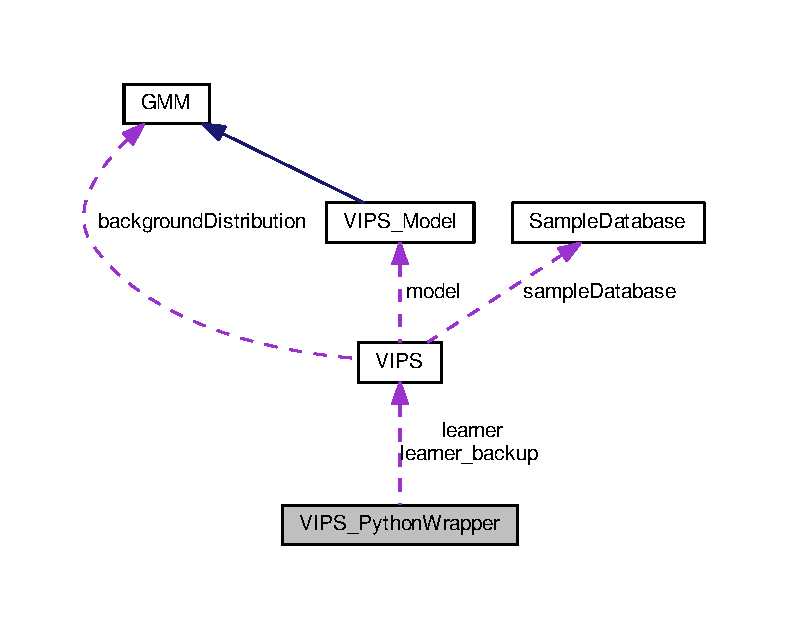
\includegraphics[width=350pt]{classVIPS__PythonWrapper__coll__graph}
\end{center}
\end{figure}
\subsection*{Public Member Functions}
\begin{DoxyCompactItemize}
\item 
{\bfseries V\+I\+P\+S\+\_\+\+Python\+Wrapper} (int num\+\_\+dimensions, int num\+\_\+threads, double min\+\_\+kl\+\_\+bound, double max\+\_\+kl\+\_\+bound)\hypertarget{classVIPS__PythonWrapper_ad5cc2281cd1d3abcd50618535c25b635}{}\label{classVIPS__PythonWrapper_ad5cc2281cd1d3abcd50618535c25b635}

\item 
void \hyperlink{classVIPS__PythonWrapper_a0a51f6e59a9b843e4a21262e4c119bbd}{add\+\_\+components} (double $\ast$new\+\_\+weights\+\_\+in, int new\+\_\+weights\+\_\+in\+\_\+dim1, double $\ast$new\+\_\+means\+\_\+in, int new\+\_\+means\+\_\+in\+\_\+dim1, int new\+\_\+means\+\_\+in\+\_\+dim2, double $\ast$new\+\_\+covs\+\_\+in, int new\+\_\+covs\+\_\+in\+\_\+dim1, int new\+\_\+covs\+\_\+in\+\_\+dim2, int new\+\_\+covs\+\_\+in\+\_\+dim3)
\item 
void \hyperlink{classVIPS__PythonWrapper_a8b17b5e96e7535358411ab8adcbcd934}{promote\+\_\+samples\+\_\+to\+\_\+components} (int N, double max\+\_\+exploration\+\_\+bonus, double tau, bool only\+\_\+check\+\_\+active\+\_\+samples, int max\+\_\+samples, bool scale\+\_\+entropy=true, bool isotropic=false)
\item 
void {\bfseries delete\+\_\+low\+\_\+weight\+\_\+components} (double min\+\_\+weight, int n\+\_\+del=300)\hypertarget{classVIPS__PythonWrapper_aeff812cf743741fcfce1871331ea14fb}{}\label{classVIPS__PythonWrapper_aeff812cf743741fcfce1871331ea14fb}

\item 
void \hyperlink{classVIPS__PythonWrapper_ac0ae21747614c8e406953e9151578053}{draw\+\_\+samples} (double N, double temperature, double $\ast$$\ast$samples\+\_\+out\+\_\+ptr, int $\ast$samples\+\_\+out\+\_\+dim1, int $\ast$samples\+\_\+out\+\_\+dim2, int $\ast$$\ast$indices\+\_\+out, int $\ast$indices\+\_\+out\+\_\+dim1)
\item 
void \hyperlink{classVIPS__PythonWrapper_adc5d4067954f4164c25426e032b5335d}{draw\+\_\+samples\+\_\+weights} (double N, double $\ast$new\+\_\+weights\+\_\+in, int new\+\_\+weights\+\_\+in\+\_\+dim1, double $\ast$$\ast$samples\+\_\+out\+\_\+ptr, int $\ast$samples\+\_\+out\+\_\+dim1, int $\ast$samples\+\_\+out\+\_\+dim2, int $\ast$$\ast$indices\+\_\+out, int $\ast$indices\+\_\+out\+\_\+dim1)
\item 
void \hyperlink{classVIPS__PythonWrapper_a9c0a069ddf27394166c523834677165a}{add\+\_\+samples\+\_\+mean\+\_\+cov} (double $\ast$samples\+\_\+ptr, int samples\+\_\+dim1, int samples\+\_\+dim2, double $\ast$target\+\_\+densities\+\_\+ptr, int td\+\_\+dim1, double $\ast$mean\+\_\+in, int mean\+\_\+in\+\_\+dim1, double $\ast$cov\+\_\+in, int cov\+\_\+in\+\_\+dim1, int cov\+\_\+in\+\_\+dim2)
\item 
void \hyperlink{classVIPS__PythonWrapper_a5a54eb8d14b32740b286f5f91660b6c2}{add\+\_\+samples} (double $\ast$samples\+\_\+ptr, int samples\+\_\+dim1, int samples\+\_\+dim2, int $\ast$indices\+\_\+ptr, int indices\+\_\+dim1, double $\ast$target\+\_\+densities\+\_\+ptr, int td\+\_\+dim1)
\item 
void \hyperlink{classVIPS__PythonWrapper_a1a2c8975cee0e96085040518a871184c}{activate\+\_\+newest\+\_\+samples} (int N, bool keep\+\_\+old)
\item 
void \hyperlink{classVIPS__PythonWrapper_ad93d42f4b18f28193aaba35129e7c068}{select\+\_\+active\+\_\+samples} (int num\+\_\+comps, int num\+\_\+samples, double temperature, double $\ast$$\ast$num\+\_\+eff\+\_\+out\+\_\+ptr, int $\ast$num\+\_\+eff\+\_\+out\+\_\+dim1)
\item 
void \hyperlink{classVIPS__PythonWrapper_a0e0bab32cbad5c82966440fd5d7e91db}{update\+\_\+targets\+\_\+for\+\_\+\+K\+L\+\_\+bounds} (bool update\+\_\+weight\+\_\+targets, bool update\+\_\+comp\+\_\+targets)
\item 
void \hyperlink{classVIPS__PythonWrapper_a79046b01fe1129abfd723c4d48ca1d45}{update\+\_\+weights} (double epsilon, double tau, double max\+\_\+entropy\+\_\+decrease, bool be\+\_\+greedy)
\item 
void \hyperlink{classVIPS__PythonWrapper_ae5a7f4052cffe00c4fee8950387af61d}{apply\+\_\+lower\+\_\+bound\+\_\+on\+\_\+weights} (double $\ast$lb\+\_\+weights\+\_\+in, int lb\+\_\+weights\+\_\+in\+\_\+dim1)
\item 
void \hyperlink{classVIPS__PythonWrapper_a948b081338679c050ed174c6598383d3}{update\+\_\+components} (double tau, double ridge\+\_\+coefficient, double max\+\_\+entropy\+\_\+decrease, double max\+\_\+active\+\_\+samples, bool dont\+\_\+learn\+\_\+correlations, bool dont\+\_\+recompute\+\_\+densities, bool adapt\+\_\+ridge\+\_\+multipliers)
\item 
void \hyperlink{classVIPS__PythonWrapper_abf63652a9d7589cc189837ba41bcf322}{recompute\+\_\+densities} (bool only\+\_\+weights\+\_\+changed)
\item 
void \hyperlink{classVIPS__PythonWrapper_acb7c2dea0de7913cc96a8d9511cd96a8}{get\+\_\+model} (double $\ast$$\ast$weights\+\_\+out\+\_\+ptr, int $\ast$weights\+\_\+out\+\_\+dim1, double $\ast$$\ast$means\+\_\+out\+\_\+ptr, int $\ast$means\+\_\+out\+\_\+dim1, int $\ast$means\+\_\+out\+\_\+dim2, double $\ast$$\ast$covs\+\_\+out\+\_\+ptr, int $\ast$covs\+\_\+out\+\_\+dim1, int $\ast$covs\+\_\+out\+\_\+dim2, int $\ast$covs\+\_\+out\+\_\+dim3)
\item 
void \hyperlink{classVIPS__PythonWrapper_acaee5a15878205a9ad0ce90c0ffbbdec}{get\+\_\+model\+\_\+entropies} (double $\ast$$\ast$entropies\+\_\+out\+\_\+ptr, int $\ast$entropies\+\_\+out\+\_\+dim1)
\item 
void \hyperlink{classVIPS__PythonWrapper_a2cf72db0bbb7259955d9229ab768cf6b}{get\+\_\+background} (double $\ast$$\ast$weights\+\_\+out\+\_\+ptr, int $\ast$weights\+\_\+out\+\_\+dim1, double $\ast$$\ast$means\+\_\+out\+\_\+ptr, int $\ast$means\+\_\+out\+\_\+dim1, int $\ast$means\+\_\+out\+\_\+dim2, double $\ast$$\ast$covs\+\_\+out\+\_\+ptr, int $\ast$covs\+\_\+out\+\_\+dim1, int $\ast$covs\+\_\+out\+\_\+dim2, int $\ast$covs\+\_\+out\+\_\+dim3)
\item 
void \hyperlink{classVIPS__PythonWrapper_aa48468dd40833596d32e202fade3af84}{get\+\_\+last\+\_\+\+K\+Ls} (double $\ast$K\+L\+\_\+weights\+\_\+out, double $\ast$$\ast$kls\+\_\+comp\+\_\+out, int $\ast$kls\+\_\+comp\+\_\+out\+\_\+dim1)
\item 
void \hyperlink{classVIPS__PythonWrapper_a6533e3114818b6dc596a51bb8d8aae32}{get\+\_\+weights} (double $\ast$$\ast$weights\+\_\+out\+\_\+ptr, int $\ast$weights\+\_\+out\+\_\+dim1, double $\ast$$\ast$log\+\_\+weights\+\_\+out\+\_\+ptr, int $\ast$log\+\_\+weights\+\_\+out\+\_\+dim1)
\item 
void \hyperlink{classVIPS__PythonWrapper_aa650a92bb89042882d548a16fdf46205}{get\+\_\+num\+\_\+samples} (int $\ast$num\+\_\+samples, int $\ast$num\+\_\+samples\+\_\+total)
\item 
void \hyperlink{classVIPS__PythonWrapper_acafd12e5bc30f51b703a73606d76de40}{get\+\_\+expected\+\_\+rewards} (double $\ast$$\ast$expected\+\_\+rewards\+\_\+out, int $\ast$expected\+\_\+rewards\+\_\+out\+\_\+dim1, double $\ast$$\ast$expected\+\_\+target\+\_\+densities\+\_\+out, int $\ast$expected\+\_\+target\+\_\+densities\+\_\+out\+\_\+dim1, double $\ast$$\ast$comp\+\_\+etd\+\_\+history\+\_\+out\+\_\+ptr, int $\ast$comp\+\_\+etd\+\_\+history\+\_\+out\+\_\+dim1, int $\ast$comp\+\_\+etd\+\_\+history\+\_\+out\+\_\+dim2, double $\ast$$\ast$comp\+\_\+reward\+\_\+history\+\_\+out\+\_\+ptr, int $\ast$comp\+\_\+reward\+\_\+history\+\_\+out\+\_\+dim1, int $\ast$comp\+\_\+reward\+\_\+history\+\_\+out\+\_\+dim2)
\item 
void \hyperlink{classVIPS__PythonWrapper_a84f192f13f7e83da0fff4801121a49c3}{get\+\_\+best\+\_\+interpolation} (int index, double $\ast$samples\+\_\+ptr, int samples\+\_\+dim1, int samples\+\_\+dim2, double $\ast$target\+\_\+densities\+\_\+ptr, int td\+\_\+dim1, double $\ast$target\+\_\+densities2\+\_\+ptr, int td2\+\_\+dim1, double scaling\+\_\+factor)
\item 
void \hyperlink{classVIPS__PythonWrapper_a4cd577f2c0ae57ba85fff0746f7c7d7a}{get\+\_\+log\+\_\+densities\+\_\+on\+\_\+mixture} (double $\ast$samples\+\_\+ptr, int samples\+\_\+dim1, int samples\+\_\+dim2, double $\ast$$\ast$sample\+\_\+densities\+\_\+out, int $\ast$sample\+\_\+densities\+\_\+out\+\_\+dim1)
\item 
void \hyperlink{classVIPS__PythonWrapper_a2be7ce5aaa742d979b35ade922139894}{get\+\_\+entropy\+\_\+estimate\+\_\+on\+\_\+active\+\_\+samples} (double $\ast$entropy)
\item 
void \hyperlink{classVIPS__PythonWrapper_a8065f48c6060b03eaa2b5c7f1f89c636}{get\+\_\+entropy\+\_\+estimate\+\_\+on\+\_\+gmm\+\_\+samples} (double $\ast$entropy, int num\+\_\+samples=10000)
\item 
void \hyperlink{classVIPS__PythonWrapper_aeef466a77710252e595fcd6e9909f975}{get\+\_\+num\+\_\+components} (int $\ast$num\+\_\+components\+\_\+out)
\item 
void \hyperlink{classVIPS__PythonWrapper_a64a647b24326d512082dbb60932eaa29}{get\+\_\+debug\+\_\+info} (double $\ast$$\ast$samples\+\_\+out\+\_\+ptr, int $\ast$samples\+\_\+out\+\_\+dim1, int $\ast$samples\+\_\+out\+\_\+dim2, double $\ast$$\ast$target\+\_\+densities\+\_\+out\+\_\+ptr, int $\ast$target\+\_\+densities\+\_\+out\+\_\+dim1, double $\ast$$\ast$log\+\_\+densities\+\_\+on\+\_\+model\+\_\+comps\+\_\+out\+\_\+ptr, int $\ast$log\+\_\+densities\+\_\+on\+\_\+model\+\_\+comps\+\_\+out\+\_\+dim1, int $\ast$log\+\_\+densities\+\_\+on\+\_\+model\+\_\+comps\+\_\+out\+\_\+dim2, double $\ast$$\ast$log\+\_\+joint\+\_\+densities\+\_\+out\+\_\+ptr, int $\ast$log\+\_\+joint\+\_\+densities\+\_\+out\+\_\+dim1, int $\ast$log\+\_\+joint\+\_\+densities\+\_\+out\+\_\+dim2, double $\ast$$\ast$log\+\_\+densities\+\_\+on\+\_\+model\+\_\+out\+\_\+ptr, int $\ast$log\+\_\+densities\+\_\+on\+\_\+model\+\_\+out\+\_\+dim1, double $\ast$$\ast$log\+\_\+responsibilities\+\_\+out\+\_\+ptr, int $\ast$log\+\_\+responsibilities\+\_\+out\+\_\+dim1, int $\ast$log\+\_\+responsibilities\+\_\+out\+\_\+dim2, double $\ast$$\ast$log\+\_\+densities\+\_\+on\+\_\+background\+\_\+out\+\_\+ptr, int $\ast$log\+\_\+densities\+\_\+on\+\_\+background\+\_\+out\+\_\+dim1, double $\ast$$\ast$importance\+\_\+weights\+\_\+out\+\_\+ptr, int $\ast$importance\+\_\+weights\+\_\+out\+\_\+dim1, int $\ast$importance\+\_\+weights\+\_\+out\+\_\+dim2, double $\ast$$\ast$importance\+\_\+weights\+\_\+normalized\+\_\+out\+\_\+ptr, int $\ast$importance\+\_\+weights\+\_\+normalized\+\_\+out\+\_\+dim1, int $\ast$importance\+\_\+weights\+\_\+normalized\+\_\+out\+\_\+dim2, int $\ast$$\ast$indices\+\_\+out, int $\ast$indices\+\_\+out\+\_\+dim1, int $\ast$$\ast$num\+\_\+samples\+\_\+history\+\_\+out\+\_\+ptr, int $\ast$num\+\_\+samples\+\_\+history\+\_\+out\+\_\+dim1, int $\ast$num\+\_\+samples\+\_\+history\+\_\+out\+\_\+dim2)
\item 
void \hyperlink{classVIPS__PythonWrapper_a8d258a474d63f442b89358c1793ccf7e}{compute\+\_\+\+K\+Ls\+\_\+between\+\_\+\+G\+M\+M\+\_\+and\+\_\+\+D\+B\+\_\+components} (bool reverse\+\_\+\+KL, float $\ast$$\ast$K\+L\+\_\+mat\+\_\+out\+\_\+ptr, int $\ast$K\+L\+\_\+mat\+\_\+out\+\_\+dim1, int $\ast$K\+L\+\_\+mat\+\_\+out\+\_\+dim2)
\item 
void \hyperlink{classVIPS__PythonWrapper_a007140eac0ea0ea69de16a7eb8c13293}{backup\+\_\+learner} ()
\item 
void \hyperlink{classVIPS__PythonWrapper_a3819321597ef3f522bd577f479ff81b0}{restore\+\_\+learner} ()
\end{DoxyCompactItemize}
\subsection*{Protected Attributes}
\begin{DoxyCompactItemize}
\item 
\hyperlink{classVIPS}{V\+I\+PS} {\bfseries learner}\hypertarget{classVIPS__PythonWrapper_a967a73404906831a828f926b4fc8c7b2}{}\label{classVIPS__PythonWrapper_a967a73404906831a828f926b4fc8c7b2}

\item 
\hyperlink{classVIPS}{V\+I\+PS} {\bfseries learner\+\_\+backup}\hypertarget{classVIPS__PythonWrapper_aaa74d7a0f9b7039f49cd7736f0fd463a}{}\label{classVIPS__PythonWrapper_aaa74d7a0f9b7039f49cd7736f0fd463a}

\item 
int {\bfseries num\+\_\+dimensions}\hypertarget{classVIPS__PythonWrapper_ae70db7c8f890fe7bba73c15de92e9d0b}{}\label{classVIPS__PythonWrapper_ae70db7c8f890fe7bba73c15de92e9d0b}

\item 
arma\+::vec {\bfseries last\+\_\+\+K\+Ls\+\_\+components}\hypertarget{classVIPS__PythonWrapper_a0d7e2c9449dc4411ba71d623c8a4d236}{}\label{classVIPS__PythonWrapper_a0d7e2c9449dc4411ba71d623c8a4d236}

\item 
double {\bfseries last\+\_\+\+K\+L\+\_\+weights}\hypertarget{classVIPS__PythonWrapper_aa37f34c104c8b41f3d8fd7a1023da696}{}\label{classVIPS__PythonWrapper_aa37f34c104c8b41f3d8fd7a1023da696}

\item 
arma\+::vec {\bfseries last\+\_\+expected\+\_\+rew}\hypertarget{classVIPS__PythonWrapper_ad33747fdb016a926ab1ea3524aa2b36b}{}\label{classVIPS__PythonWrapper_ad33747fdb016a926ab1ea3524aa2b36b}

\item 
arma\+::vec {\bfseries last\+\_\+expected\+\_\+target\+\_\+densities}\hypertarget{classVIPS__PythonWrapper_afd270b0737302fb8a3e755057f4363c2}{}\label{classVIPS__PythonWrapper_afd270b0737302fb8a3e755057f4363c2}

\end{DoxyCompactItemize}


\subsection{Member Function Documentation}
\index{V\+I\+P\+S\+\_\+\+Python\+Wrapper@{V\+I\+P\+S\+\_\+\+Python\+Wrapper}!activate\+\_\+newest\+\_\+samples@{activate\+\_\+newest\+\_\+samples}}
\index{activate\+\_\+newest\+\_\+samples@{activate\+\_\+newest\+\_\+samples}!V\+I\+P\+S\+\_\+\+Python\+Wrapper@{V\+I\+P\+S\+\_\+\+Python\+Wrapper}}
\subsubsection[{\texorpdfstring{activate\+\_\+newest\+\_\+samples(int N, bool keep\+\_\+old)}{activate_newest_samples(int N, bool keep_old)}}]{\setlength{\rightskip}{0pt plus 5cm}void V\+I\+P\+S\+\_\+\+Python\+Wrapper\+::activate\+\_\+newest\+\_\+samples (
\begin{DoxyParamCaption}
\item[{int}]{N, }
\item[{bool}]{keep\+\_\+old}
\end{DoxyParamCaption}
)}\hypertarget{classVIPS__PythonWrapper_a1a2c8975cee0e96085040518a871184c}{}\label{classVIPS__PythonWrapper_a1a2c8975cee0e96085040518a871184c}
Selects the N most recent samples and activates them (i.\+e. uses them for the upcoming learning iteration).~\newline
 Makes sure, that all relevant data (e.\+g. densities, importance weights, etc.) gets updated 
\begin{DoxyParams}{Parameters}
{\em N} & -\/ the maximum number of recent samples to be activated, actually number of activated samples might be less, iff the sample database does not contain sufficient samples.~\newline
 \\
\hline
{\em keep\+\_\+old} & -\/ iff set to true, the currently active sample will remain active \\
\hline
\end{DoxyParams}
\index{V\+I\+P\+S\+\_\+\+Python\+Wrapper@{V\+I\+P\+S\+\_\+\+Python\+Wrapper}!add\+\_\+components@{add\+\_\+components}}
\index{add\+\_\+components@{add\+\_\+components}!V\+I\+P\+S\+\_\+\+Python\+Wrapper@{V\+I\+P\+S\+\_\+\+Python\+Wrapper}}
\subsubsection[{\texorpdfstring{add\+\_\+components(double $\ast$new\+\_\+weights\+\_\+in, int new\+\_\+weights\+\_\+in\+\_\+dim1, double $\ast$new\+\_\+means\+\_\+in, int new\+\_\+means\+\_\+in\+\_\+dim1, int new\+\_\+means\+\_\+in\+\_\+dim2, double $\ast$new\+\_\+covs\+\_\+in, int new\+\_\+covs\+\_\+in\+\_\+dim1, int new\+\_\+covs\+\_\+in\+\_\+dim2, int new\+\_\+covs\+\_\+in\+\_\+dim3)}{add_components(double *new_weights_in, int new_weights_in_dim1, double *new_means_in, int new_means_in_dim1, int new_means_in_dim2, double *new_covs_in, int new_covs_in_dim1, int new_covs_in_dim2, int new_covs_in_dim3)}}]{\setlength{\rightskip}{0pt plus 5cm}void V\+I\+P\+S\+\_\+\+Python\+Wrapper\+::add\+\_\+components (
\begin{DoxyParamCaption}
\item[{double $\ast$}]{new\+\_\+weights\+\_\+in, }
\item[{int}]{new\+\_\+weights\+\_\+in\+\_\+dim1, }
\item[{double $\ast$}]{new\+\_\+means\+\_\+in, }
\item[{int}]{new\+\_\+means\+\_\+in\+\_\+dim1, }
\item[{int}]{new\+\_\+means\+\_\+in\+\_\+dim2, }
\item[{double $\ast$}]{new\+\_\+covs\+\_\+in, }
\item[{int}]{new\+\_\+covs\+\_\+in\+\_\+dim1, }
\item[{int}]{new\+\_\+covs\+\_\+in\+\_\+dim2, }
\item[{int}]{new\+\_\+covs\+\_\+in\+\_\+dim3}
\end{DoxyParamCaption}
)}\hypertarget{classVIPS__PythonWrapper_a0a51f6e59a9b843e4a21262e4c119bbd}{}\label{classVIPS__PythonWrapper_a0a51f6e59a9b843e4a21262e4c119bbd}
Adds new components~\newline
. 
\begin{DoxyParams}{Parameters}
{\em new\+\_\+weights} & -\/ new weights of the \hyperlink{classGMM}{G\+MM} (including existing components) \\
\hline
{\em new\+\_\+means} & -\/ matrix of size N\+\_\+dimensions x N\+\_\+new\+Components specifying the means of the new components \\
\hline
{\em new\+\_\+covs} & -\/ cube of size N\+\_\+dimensions x N\+\_\+dimensions x N\+\_\+new\+Components specifying the covariance matrices of the new components \\
\hline
\end{DoxyParams}
\index{V\+I\+P\+S\+\_\+\+Python\+Wrapper@{V\+I\+P\+S\+\_\+\+Python\+Wrapper}!add\+\_\+samples@{add\+\_\+samples}}
\index{add\+\_\+samples@{add\+\_\+samples}!V\+I\+P\+S\+\_\+\+Python\+Wrapper@{V\+I\+P\+S\+\_\+\+Python\+Wrapper}}
\subsubsection[{\texorpdfstring{add\+\_\+samples(double $\ast$samples\+\_\+ptr, int samples\+\_\+dim1, int samples\+\_\+dim2, int $\ast$indices\+\_\+ptr, int indices\+\_\+dim1, double $\ast$target\+\_\+densities\+\_\+ptr, int td\+\_\+dim1)}{add_samples(double *samples_ptr, int samples_dim1, int samples_dim2, int *indices_ptr, int indices_dim1, double *target_densities_ptr, int td_dim1)}}]{\setlength{\rightskip}{0pt plus 5cm}void V\+I\+P\+S\+\_\+\+Python\+Wrapper\+::add\+\_\+samples (
\begin{DoxyParamCaption}
\item[{double $\ast$}]{samples\+\_\+ptr, }
\item[{int}]{samples\+\_\+dim1, }
\item[{int}]{samples\+\_\+dim2, }
\item[{int $\ast$}]{indices\+\_\+ptr, }
\item[{int}]{indices\+\_\+dim1, }
\item[{double $\ast$}]{target\+\_\+densities\+\_\+ptr, }
\item[{int}]{td\+\_\+dim1}
\end{DoxyParamCaption}
)}\hypertarget{classVIPS__PythonWrapper_a5a54eb8d14b32740b286f5f91660b6c2}{}\label{classVIPS__PythonWrapper_a5a54eb8d14b32740b286f5f91660b6c2}
Adds new samples to the database. Note that the samples will not be used for learning, until they have been activated (see activate\+\_\+newest\+\_\+samples).~\newline
 The samples are assumed to have been drawn from the current model and the indices of the relevant components are to be provided for computing background distributions when necessary. 
\begin{DoxyParams}{Parameters}
{\em new\+\_\+samples} & -\/ a matrix of size N\+\_\+dimensions X N\+\_\+samples \\
\hline
{\em used\+\_\+components} & -\/ a vector of size N\+\_\+samples containing the indices of the components the corresponding samples have been drawn from \\
\hline
{\em new\+\_\+target\+\_\+densities} & -\/ a vector of size N\+\_\+samples containing the unnormalized densities on the target distribution \\
\hline
\end{DoxyParams}
\begin{DoxySeeAlso}{See also}
\hyperlink{classVIPS__PythonWrapper_a1a2c8975cee0e96085040518a871184c}{activate\+\_\+newest\+\_\+samples} 
\end{DoxySeeAlso}
\index{V\+I\+P\+S\+\_\+\+Python\+Wrapper@{V\+I\+P\+S\+\_\+\+Python\+Wrapper}!add\+\_\+samples\+\_\+mean\+\_\+cov@{add\+\_\+samples\+\_\+mean\+\_\+cov}}
\index{add\+\_\+samples\+\_\+mean\+\_\+cov@{add\+\_\+samples\+\_\+mean\+\_\+cov}!V\+I\+P\+S\+\_\+\+Python\+Wrapper@{V\+I\+P\+S\+\_\+\+Python\+Wrapper}}
\subsubsection[{\texorpdfstring{add\+\_\+samples\+\_\+mean\+\_\+cov(double $\ast$samples\+\_\+ptr, int samples\+\_\+dim1, int samples\+\_\+dim2, double $\ast$target\+\_\+densities\+\_\+ptr, int td\+\_\+dim1, double $\ast$mean\+\_\+in, int mean\+\_\+in\+\_\+dim1, double $\ast$cov\+\_\+in, int cov\+\_\+in\+\_\+dim1, int cov\+\_\+in\+\_\+dim2)}{add_samples_mean_cov(double *samples_ptr, int samples_dim1, int samples_dim2, double *target_densities_ptr, int td_dim1, double *mean_in, int mean_in_dim1, double *cov_in, int cov_in_dim1, int cov_in_dim2)}}]{\setlength{\rightskip}{0pt plus 5cm}void V\+I\+P\+S\+\_\+\+Python\+Wrapper\+::add\+\_\+samples\+\_\+mean\+\_\+cov (
\begin{DoxyParamCaption}
\item[{double $\ast$}]{samples\+\_\+ptr, }
\item[{int}]{samples\+\_\+dim1, }
\item[{int}]{samples\+\_\+dim2, }
\item[{double $\ast$}]{target\+\_\+densities\+\_\+ptr, }
\item[{int}]{td\+\_\+dim1, }
\item[{double $\ast$}]{mean\+\_\+in, }
\item[{int}]{mean\+\_\+in\+\_\+dim1, }
\item[{double $\ast$}]{cov\+\_\+in, }
\item[{int}]{cov\+\_\+in\+\_\+dim1, }
\item[{int}]{cov\+\_\+in\+\_\+dim2}
\end{DoxyParamCaption}
)}\hypertarget{classVIPS__PythonWrapper_a9c0a069ddf27394166c523834677165a}{}\label{classVIPS__PythonWrapper_a9c0a069ddf27394166c523834677165a}
Adds new samples to the database. Note that the samples will not be used for learning, until they have been activated (see activate\+\_\+newest\+\_\+samples).~\newline
 The samples are assumed to have been drawn from a Gaussian with specified mean and covariance matrix 
\begin{DoxyParams}{Parameters}
{\em new\+\_\+samples} & -\/ a matrix of size N\+\_\+dimensions X N\+\_\+samples \\
\hline
{\em new\+\_\+target\+\_\+densities} & -\/ a vector of size N\+\_\+samples containing the unnormalized densities on the target distribution \\
\hline
{\em used\+\_\+mean} & -\/ a vector containing the mean of the Gaussian used for drawing the samples \\
\hline
{\em used\+\_\+cov} & -\/ a matrix containing the covariance matrix of the Gaussian used for drawing the samples \\
\hline
\end{DoxyParams}
\begin{DoxySeeAlso}{See also}
\hyperlink{classVIPS__PythonWrapper_a1a2c8975cee0e96085040518a871184c}{activate\+\_\+newest\+\_\+samples} 
\end{DoxySeeAlso}
\index{V\+I\+P\+S\+\_\+\+Python\+Wrapper@{V\+I\+P\+S\+\_\+\+Python\+Wrapper}!apply\+\_\+lower\+\_\+bound\+\_\+on\+\_\+weights@{apply\+\_\+lower\+\_\+bound\+\_\+on\+\_\+weights}}
\index{apply\+\_\+lower\+\_\+bound\+\_\+on\+\_\+weights@{apply\+\_\+lower\+\_\+bound\+\_\+on\+\_\+weights}!V\+I\+P\+S\+\_\+\+Python\+Wrapper@{V\+I\+P\+S\+\_\+\+Python\+Wrapper}}
\subsubsection[{\texorpdfstring{apply\+\_\+lower\+\_\+bound\+\_\+on\+\_\+weights(double $\ast$lb\+\_\+weights\+\_\+in, int lb\+\_\+weights\+\_\+in\+\_\+dim1)}{apply_lower_bound_on_weights(double *lb_weights_in, int lb_weights_in_dim1)}}]{\setlength{\rightskip}{0pt plus 5cm}void V\+I\+P\+S\+\_\+\+Python\+Wrapper\+::apply\+\_\+lower\+\_\+bound\+\_\+on\+\_\+weights (
\begin{DoxyParamCaption}
\item[{double $\ast$}]{lb\+\_\+weights\+\_\+in, }
\item[{int}]{lb\+\_\+weights\+\_\+in\+\_\+dim1}
\end{DoxyParamCaption}
)}\hypertarget{classVIPS__PythonWrapper_ae5a7f4052cffe00c4fee8950387af61d}{}\label{classVIPS__PythonWrapper_ae5a7f4052cffe00c4fee8950387af61d}
Lower bounds all weights and renormalizes by scaling those weights that have not been modified. Currently, we do not check whether weights that got rescaled drop below their lower bound. 
\begin{DoxyParams}{Parameters}
{\em lb\+\_\+weights\+\_\+in} & -\/ vector containing the lower bound for all weights. The sum of lb\+\_\+weights\+\_\+in needs to be $<$= 1 \\
\hline
\end{DoxyParams}
\index{V\+I\+P\+S\+\_\+\+Python\+Wrapper@{V\+I\+P\+S\+\_\+\+Python\+Wrapper}!backup\+\_\+learner@{backup\+\_\+learner}}
\index{backup\+\_\+learner@{backup\+\_\+learner}!V\+I\+P\+S\+\_\+\+Python\+Wrapper@{V\+I\+P\+S\+\_\+\+Python\+Wrapper}}
\subsubsection[{\texorpdfstring{backup\+\_\+learner()}{backup_learner()}}]{\setlength{\rightskip}{0pt plus 5cm}void V\+I\+P\+S\+\_\+\+Python\+Wrapper\+::backup\+\_\+learner (
\begin{DoxyParamCaption}
{}
\end{DoxyParamCaption}
)}\hypertarget{classVIPS__PythonWrapper_a007140eac0ea0ea69de16a7eb8c13293}{}\label{classVIPS__PythonWrapper_a007140eac0ea0ea69de16a7eb8c13293}
creates a backup of the the current state of the learner (overwriting previous backup). \begin{DoxySeeAlso}{See also}
restore\+\_\+backup() 
\end{DoxySeeAlso}
\index{V\+I\+P\+S\+\_\+\+Python\+Wrapper@{V\+I\+P\+S\+\_\+\+Python\+Wrapper}!compute\+\_\+\+K\+Ls\+\_\+between\+\_\+\+G\+M\+M\+\_\+and\+\_\+\+D\+B\+\_\+components@{compute\+\_\+\+K\+Ls\+\_\+between\+\_\+\+G\+M\+M\+\_\+and\+\_\+\+D\+B\+\_\+components}}
\index{compute\+\_\+\+K\+Ls\+\_\+between\+\_\+\+G\+M\+M\+\_\+and\+\_\+\+D\+B\+\_\+components@{compute\+\_\+\+K\+Ls\+\_\+between\+\_\+\+G\+M\+M\+\_\+and\+\_\+\+D\+B\+\_\+components}!V\+I\+P\+S\+\_\+\+Python\+Wrapper@{V\+I\+P\+S\+\_\+\+Python\+Wrapper}}
\subsubsection[{\texorpdfstring{compute\+\_\+\+K\+Ls\+\_\+between\+\_\+\+G\+M\+M\+\_\+and\+\_\+\+D\+B\+\_\+components(bool reverse\+\_\+\+K\+L, float $\ast$$\ast$\+K\+L\+\_\+mat\+\_\+out\+\_\+ptr, int $\ast$\+K\+L\+\_\+mat\+\_\+out\+\_\+dim1, int $\ast$\+K\+L\+\_\+mat\+\_\+out\+\_\+dim2)}{compute_KLs_between_GMM_and_DB_components(bool reverse_KL, float **KL_mat_out_ptr, int *KL_mat_out_dim1, int *KL_mat_out_dim2)}}]{\setlength{\rightskip}{0pt plus 5cm}void V\+I\+P\+S\+\_\+\+Python\+Wrapper\+::compute\+\_\+\+K\+Ls\+\_\+between\+\_\+\+G\+M\+M\+\_\+and\+\_\+\+D\+B\+\_\+components (
\begin{DoxyParamCaption}
\item[{bool}]{reverse\+\_\+\+KL, }
\item[{float $\ast$$\ast$}]{K\+L\+\_\+mat\+\_\+out\+\_\+ptr, }
\item[{int $\ast$}]{K\+L\+\_\+mat\+\_\+out\+\_\+dim1, }
\item[{int $\ast$}]{K\+L\+\_\+mat\+\_\+out\+\_\+dim2}
\end{DoxyParamCaption}
)}\hypertarget{classVIPS__PythonWrapper_a8d258a474d63f442b89358c1793ccf7e}{}\label{classVIPS__PythonWrapper_a8d258a474d63f442b89358c1793ccf7e}
For each component of the current approximation compute the KL w.\+r.\+t. each component that is stored in the database. If the parameter reverse\+\_\+\+KL is set to true, computes instead the KL for each database component w.\+r.\+t. each \hyperlink{classGMM}{G\+MM} component 
\begin{DoxyParams}{Parameters}
{\em reverse\+\_\+\+KL} & -\/ if set to bool compute the KL between database\+\_\+componets w.\+r.\+t. \hyperlink{classGMM}{G\+MM} components \\
\hline
\end{DoxyParams}
\begin{DoxyReturn}{Returns}
a matrix of size components\+\_\+in\+\_\+gmm x components\+\_\+in\+\_\+database (or transposed if computing the reverse KL) containing the relative entropies. 
\end{DoxyReturn}
\index{V\+I\+P\+S\+\_\+\+Python\+Wrapper@{V\+I\+P\+S\+\_\+\+Python\+Wrapper}!draw\+\_\+samples@{draw\+\_\+samples}}
\index{draw\+\_\+samples@{draw\+\_\+samples}!V\+I\+P\+S\+\_\+\+Python\+Wrapper@{V\+I\+P\+S\+\_\+\+Python\+Wrapper}}
\subsubsection[{\texorpdfstring{draw\+\_\+samples(double N, double temperature, double $\ast$$\ast$samples\+\_\+out\+\_\+ptr, int $\ast$samples\+\_\+out\+\_\+dim1, int $\ast$samples\+\_\+out\+\_\+dim2, int $\ast$$\ast$indices\+\_\+out, int $\ast$indices\+\_\+out\+\_\+dim1)}{draw_samples(double N, double temperature, double **samples_out_ptr, int *samples_out_dim1, int *samples_out_dim2, int **indices_out, int *indices_out_dim1)}}]{\setlength{\rightskip}{0pt plus 5cm}void V\+I\+P\+S\+\_\+\+Python\+Wrapper\+::draw\+\_\+samples (
\begin{DoxyParamCaption}
\item[{double}]{N, }
\item[{double}]{temperature, }
\item[{double $\ast$$\ast$}]{samples\+\_\+out\+\_\+ptr, }
\item[{int $\ast$}]{samples\+\_\+out\+\_\+dim1, }
\item[{int $\ast$}]{samples\+\_\+out\+\_\+dim2, }
\item[{int $\ast$$\ast$}]{indices\+\_\+out, }
\item[{int $\ast$}]{indices\+\_\+out\+\_\+dim1}
\end{DoxyParamCaption}
)}\hypertarget{classVIPS__PythonWrapper_ac0ae21747614c8e406953e9151578053}{}\label{classVIPS__PythonWrapper_ac0ae21747614c8e406953e9151578053}
Sample from the current \hyperlink{classGMM}{G\+MM} approximation, but use the specified temperature to to adapt the weights, i.\+e. the coefficient are replaced by p\textquotesingle{}(o)  exp(log(p(o)$\ast$temperature)) 
\begin{DoxyParams}{Parameters}
{\em N} & -\/ the numb er of samples to been drawn \\
\hline
{\em weights} & -\/ the weights (coefficients) to be used \\
\hline
\end{DoxyParams}
\begin{DoxyReturn}{Returns}
samples -\/ N Samples drwan from the mixture with the given weights 

indices -\/ for each sample, the index of the component that was used for drawing it 
\end{DoxyReturn}
\index{V\+I\+P\+S\+\_\+\+Python\+Wrapper@{V\+I\+P\+S\+\_\+\+Python\+Wrapper}!draw\+\_\+samples\+\_\+weights@{draw\+\_\+samples\+\_\+weights}}
\index{draw\+\_\+samples\+\_\+weights@{draw\+\_\+samples\+\_\+weights}!V\+I\+P\+S\+\_\+\+Python\+Wrapper@{V\+I\+P\+S\+\_\+\+Python\+Wrapper}}
\subsubsection[{\texorpdfstring{draw\+\_\+samples\+\_\+weights(double N, double $\ast$new\+\_\+weights\+\_\+in, int new\+\_\+weights\+\_\+in\+\_\+dim1, double $\ast$$\ast$samples\+\_\+out\+\_\+ptr, int $\ast$samples\+\_\+out\+\_\+dim1, int $\ast$samples\+\_\+out\+\_\+dim2, int $\ast$$\ast$indices\+\_\+out, int $\ast$indices\+\_\+out\+\_\+dim1)}{draw_samples_weights(double N, double *new_weights_in, int new_weights_in_dim1, double **samples_out_ptr, int *samples_out_dim1, int *samples_out_dim2, int **indices_out, int *indices_out_dim1)}}]{\setlength{\rightskip}{0pt plus 5cm}void V\+I\+P\+S\+\_\+\+Python\+Wrapper\+::draw\+\_\+samples\+\_\+weights (
\begin{DoxyParamCaption}
\item[{double}]{N, }
\item[{double $\ast$}]{new\+\_\+weights\+\_\+in, }
\item[{int}]{new\+\_\+weights\+\_\+in\+\_\+dim1, }
\item[{double $\ast$$\ast$}]{samples\+\_\+out\+\_\+ptr, }
\item[{int $\ast$}]{samples\+\_\+out\+\_\+dim1, }
\item[{int $\ast$}]{samples\+\_\+out\+\_\+dim2, }
\item[{int $\ast$$\ast$}]{indices\+\_\+out, }
\item[{int $\ast$}]{indices\+\_\+out\+\_\+dim1}
\end{DoxyParamCaption}
)}\hypertarget{classVIPS__PythonWrapper_adc5d4067954f4164c25426e032b5335d}{}\label{classVIPS__PythonWrapper_adc5d4067954f4164c25426e032b5335d}
Sample from the current \hyperlink{classGMM}{G\+MM} approximation, but use the specified component coefficients. 
\begin{DoxyParams}{Parameters}
{\em N} & -\/ the numb er of samples to been drawn \\
\hline
{\em weights} & -\/ the weights (coefficients) to be used \\
\hline
\end{DoxyParams}
\begin{DoxyReturn}{Returns}
samples -\/ N Samples drwan from the mixture with the given weights 

indices -\/ for each sample, the index of the component that was used for drawing it 
\end{DoxyReturn}
\index{V\+I\+P\+S\+\_\+\+Python\+Wrapper@{V\+I\+P\+S\+\_\+\+Python\+Wrapper}!get\+\_\+background@{get\+\_\+background}}
\index{get\+\_\+background@{get\+\_\+background}!V\+I\+P\+S\+\_\+\+Python\+Wrapper@{V\+I\+P\+S\+\_\+\+Python\+Wrapper}}
\subsubsection[{\texorpdfstring{get\+\_\+background(double $\ast$$\ast$weights\+\_\+out\+\_\+ptr, int $\ast$weights\+\_\+out\+\_\+dim1, double $\ast$$\ast$means\+\_\+out\+\_\+ptr, int $\ast$means\+\_\+out\+\_\+dim1, int $\ast$means\+\_\+out\+\_\+dim2, double $\ast$$\ast$covs\+\_\+out\+\_\+ptr, int $\ast$covs\+\_\+out\+\_\+dim1, int $\ast$covs\+\_\+out\+\_\+dim2, int $\ast$covs\+\_\+out\+\_\+dim3)}{get_background(double **weights_out_ptr, int *weights_out_dim1, double **means_out_ptr, int *means_out_dim1, int *means_out_dim2, double **covs_out_ptr, int *covs_out_dim1, int *covs_out_dim2, int *covs_out_dim3)}}]{\setlength{\rightskip}{0pt plus 5cm}void V\+I\+P\+S\+\_\+\+Python\+Wrapper\+::get\+\_\+background (
\begin{DoxyParamCaption}
\item[{double $\ast$$\ast$}]{weights\+\_\+out\+\_\+ptr, }
\item[{int $\ast$}]{weights\+\_\+out\+\_\+dim1, }
\item[{double $\ast$$\ast$}]{means\+\_\+out\+\_\+ptr, }
\item[{int $\ast$}]{means\+\_\+out\+\_\+dim1, }
\item[{int $\ast$}]{means\+\_\+out\+\_\+dim2, }
\item[{double $\ast$$\ast$}]{covs\+\_\+out\+\_\+ptr, }
\item[{int $\ast$}]{covs\+\_\+out\+\_\+dim1, }
\item[{int $\ast$}]{covs\+\_\+out\+\_\+dim2, }
\item[{int $\ast$}]{covs\+\_\+out\+\_\+dim3}
\end{DoxyParamCaption}
)}\hypertarget{classVIPS__PythonWrapper_a2cf72db0bbb7259955d9229ab768cf6b}{}\label{classVIPS__PythonWrapper_a2cf72db0bbb7259955d9229ab768cf6b}
Returns the background distribution used for computing importance weights. \begin{DoxyReturn}{Returns}
weights -\/ weights for each component 

means -\/ means for each component 

covs -\/ covariance matrices for each component 
\end{DoxyReturn}
\index{V\+I\+P\+S\+\_\+\+Python\+Wrapper@{V\+I\+P\+S\+\_\+\+Python\+Wrapper}!get\+\_\+best\+\_\+interpolation@{get\+\_\+best\+\_\+interpolation}}
\index{get\+\_\+best\+\_\+interpolation@{get\+\_\+best\+\_\+interpolation}!V\+I\+P\+S\+\_\+\+Python\+Wrapper@{V\+I\+P\+S\+\_\+\+Python\+Wrapper}}
\subsubsection[{\texorpdfstring{get\+\_\+best\+\_\+interpolation(int index, double $\ast$samples\+\_\+ptr, int samples\+\_\+dim1, int samples\+\_\+dim2, double $\ast$target\+\_\+densities\+\_\+ptr, int td\+\_\+dim1, double $\ast$target\+\_\+densities2\+\_\+ptr, int td2\+\_\+dim1, double scaling\+\_\+factor)}{get_best_interpolation(int index, double *samples_ptr, int samples_dim1, int samples_dim2, double *target_densities_ptr, int td_dim1, double *target_densities2_ptr, int td2_dim1, double scaling_factor)}}]{\setlength{\rightskip}{0pt plus 5cm}void V\+I\+P\+S\+\_\+\+Python\+Wrapper\+::get\+\_\+best\+\_\+interpolation (
\begin{DoxyParamCaption}
\item[{int}]{index, }
\item[{double $\ast$}]{samples\+\_\+ptr, }
\item[{int}]{samples\+\_\+dim1, }
\item[{int}]{samples\+\_\+dim2, }
\item[{double $\ast$}]{target\+\_\+densities\+\_\+ptr, }
\item[{int}]{td\+\_\+dim1, }
\item[{double $\ast$}]{target\+\_\+densities2\+\_\+ptr, }
\item[{int}]{td2\+\_\+dim1, }
\item[{double}]{scaling\+\_\+factor}
\end{DoxyParamCaption}
)}\hypertarget{classVIPS__PythonWrapper_a84f192f13f7e83da0fff4801121a49c3}{}\label{classVIPS__PythonWrapper_a84f192f13f7e83da0fff4801121a49c3}
For a given component, find the best interpolation between the current covariance matrix and a spherical one using a linear linesearch. ~\newline
 The quality of the covariance matrix is estimated based on an importance weighted Monte Carlo estimate of the expected loglikelihood on the target distribution. ~\newline
 The Monte Carlo estimate is computed based on a given set of samples, the corresponding target loglikelihoods and the loglikelihood of the sampling distribution. ~\newline
 I\+M\+P\+O\+R\+T\+A\+NT\+: This method will change the component to the best interpolation. ~\newline
 
\begin{DoxyParams}{Parameters}
{\em index} & -\/ index specifying which component of the current model should be adapted ~\newline
 \\
\hline
{\em samples\+\_\+ptr} & -\/ samples for the Monte Carlo estimate ~\newline
 \\
\hline
{\em target\+\_\+densities\+\_\+ptr} & -\/ vector containing the loglikelihood under the target distribution for each sample ~\newline
 \\
\hline
{\em target\+\_\+densities2\+\_\+ptr} & -\/ vector containing the loglikelihood of the distribution that was used for drawing the samples ~\newline
 \\
\hline
{\em scaling\+\_\+factor} & -\/ the spherical covariance matrix is given by scaling\+\_\+factor $\ast$ eye() ~\newline
 \\
\hline
\end{DoxyParams}
\index{V\+I\+P\+S\+\_\+\+Python\+Wrapper@{V\+I\+P\+S\+\_\+\+Python\+Wrapper}!get\+\_\+debug\+\_\+info@{get\+\_\+debug\+\_\+info}}
\index{get\+\_\+debug\+\_\+info@{get\+\_\+debug\+\_\+info}!V\+I\+P\+S\+\_\+\+Python\+Wrapper@{V\+I\+P\+S\+\_\+\+Python\+Wrapper}}
\subsubsection[{\texorpdfstring{get\+\_\+debug\+\_\+info(double $\ast$$\ast$samples\+\_\+out\+\_\+ptr, int $\ast$samples\+\_\+out\+\_\+dim1, int $\ast$samples\+\_\+out\+\_\+dim2, double $\ast$$\ast$target\+\_\+densities\+\_\+out\+\_\+ptr, int $\ast$target\+\_\+densities\+\_\+out\+\_\+dim1, double $\ast$$\ast$log\+\_\+densities\+\_\+on\+\_\+model\+\_\+comps\+\_\+out\+\_\+ptr, int $\ast$log\+\_\+densities\+\_\+on\+\_\+model\+\_\+comps\+\_\+out\+\_\+dim1, int $\ast$log\+\_\+densities\+\_\+on\+\_\+model\+\_\+comps\+\_\+out\+\_\+dim2, double $\ast$$\ast$log\+\_\+joint\+\_\+densities\+\_\+out\+\_\+ptr, int $\ast$log\+\_\+joint\+\_\+densities\+\_\+out\+\_\+dim1, int $\ast$log\+\_\+joint\+\_\+densities\+\_\+out\+\_\+dim2, double $\ast$$\ast$log\+\_\+densities\+\_\+on\+\_\+model\+\_\+out\+\_\+ptr, int $\ast$log\+\_\+densities\+\_\+on\+\_\+model\+\_\+out\+\_\+dim1, double $\ast$$\ast$log\+\_\+responsibilities\+\_\+out\+\_\+ptr, int $\ast$log\+\_\+responsibilities\+\_\+out\+\_\+dim1, int $\ast$log\+\_\+responsibilities\+\_\+out\+\_\+dim2, double $\ast$$\ast$log\+\_\+densities\+\_\+on\+\_\+background\+\_\+out\+\_\+ptr, int $\ast$log\+\_\+densities\+\_\+on\+\_\+background\+\_\+out\+\_\+dim1, double $\ast$$\ast$importance\+\_\+weights\+\_\+out\+\_\+ptr, int $\ast$importance\+\_\+weights\+\_\+out\+\_\+dim1, int $\ast$importance\+\_\+weights\+\_\+out\+\_\+dim2, double $\ast$$\ast$importance\+\_\+weights\+\_\+normalized\+\_\+out\+\_\+ptr, int $\ast$importance\+\_\+weights\+\_\+normalized\+\_\+out\+\_\+dim1, int $\ast$importance\+\_\+weights\+\_\+normalized\+\_\+out\+\_\+dim2, int $\ast$$\ast$indices\+\_\+out, int $\ast$indices\+\_\+out\+\_\+dim1, int $\ast$$\ast$num\+\_\+samples\+\_\+history\+\_\+out\+\_\+ptr, int $\ast$num\+\_\+samples\+\_\+history\+\_\+out\+\_\+dim1, int $\ast$num\+\_\+samples\+\_\+history\+\_\+out\+\_\+dim2)}{get_debug_info(double **samples_out_ptr, int *samples_out_dim1, int *samples_out_dim2, double **target_densities_out_ptr, int *target_densities_out_dim1, double **log_densities_on_model_comps_out_ptr, int *log_densities_on_model_comps_out_dim1, int *log_densities_on_model_comps_out_dim2, double **log_joint_densities_out_ptr, int *log_joint_densities_out_dim1, int *log_joint_densities_out_dim2, double **log_densities_on_model_out_ptr, int *log_densities_on_model_out_dim1, double **log_responsibilities_out_ptr, int *log_responsibilities_out_dim1, int *log_responsibilities_out_dim2, double **log_densities_on_background_out_ptr, int *log_densities_on_background_out_dim1, double **importance_weights_out_ptr, int *importance_weights_out_dim1, int *importance_weights_out_dim2, double **importance_weights_normalized_out_ptr, int *importance_weights_normalized_out_dim1, int *importance_weights_normalized_out_dim2, int **indices_out, int *indices_out_dim1, int **num_samples_history_out_ptr, int *num_samples_history_out_dim1, int *num_samples_history_out_dim2)}}]{\setlength{\rightskip}{0pt plus 5cm}void V\+I\+P\+S\+\_\+\+Python\+Wrapper\+::get\+\_\+debug\+\_\+info (
\begin{DoxyParamCaption}
\item[{double $\ast$$\ast$}]{samples\+\_\+out\+\_\+ptr, }
\item[{int $\ast$}]{samples\+\_\+out\+\_\+dim1, }
\item[{int $\ast$}]{samples\+\_\+out\+\_\+dim2, }
\item[{double $\ast$$\ast$}]{target\+\_\+densities\+\_\+out\+\_\+ptr, }
\item[{int $\ast$}]{target\+\_\+densities\+\_\+out\+\_\+dim1, }
\item[{double $\ast$$\ast$}]{log\+\_\+densities\+\_\+on\+\_\+model\+\_\+comps\+\_\+out\+\_\+ptr, }
\item[{int $\ast$}]{log\+\_\+densities\+\_\+on\+\_\+model\+\_\+comps\+\_\+out\+\_\+dim1, }
\item[{int $\ast$}]{log\+\_\+densities\+\_\+on\+\_\+model\+\_\+comps\+\_\+out\+\_\+dim2, }
\item[{double $\ast$$\ast$}]{log\+\_\+joint\+\_\+densities\+\_\+out\+\_\+ptr, }
\item[{int $\ast$}]{log\+\_\+joint\+\_\+densities\+\_\+out\+\_\+dim1, }
\item[{int $\ast$}]{log\+\_\+joint\+\_\+densities\+\_\+out\+\_\+dim2, }
\item[{double $\ast$$\ast$}]{log\+\_\+densities\+\_\+on\+\_\+model\+\_\+out\+\_\+ptr, }
\item[{int $\ast$}]{log\+\_\+densities\+\_\+on\+\_\+model\+\_\+out\+\_\+dim1, }
\item[{double $\ast$$\ast$}]{log\+\_\+responsibilities\+\_\+out\+\_\+ptr, }
\item[{int $\ast$}]{log\+\_\+responsibilities\+\_\+out\+\_\+dim1, }
\item[{int $\ast$}]{log\+\_\+responsibilities\+\_\+out\+\_\+dim2, }
\item[{double $\ast$$\ast$}]{log\+\_\+densities\+\_\+on\+\_\+background\+\_\+out\+\_\+ptr, }
\item[{int $\ast$}]{log\+\_\+densities\+\_\+on\+\_\+background\+\_\+out\+\_\+dim1, }
\item[{double $\ast$$\ast$}]{importance\+\_\+weights\+\_\+out\+\_\+ptr, }
\item[{int $\ast$}]{importance\+\_\+weights\+\_\+out\+\_\+dim1, }
\item[{int $\ast$}]{importance\+\_\+weights\+\_\+out\+\_\+dim2, }
\item[{double $\ast$$\ast$}]{importance\+\_\+weights\+\_\+normalized\+\_\+out\+\_\+ptr, }
\item[{int $\ast$}]{importance\+\_\+weights\+\_\+normalized\+\_\+out\+\_\+dim1, }
\item[{int $\ast$}]{importance\+\_\+weights\+\_\+normalized\+\_\+out\+\_\+dim2, }
\item[{int $\ast$$\ast$}]{indices\+\_\+out, }
\item[{int $\ast$}]{indices\+\_\+out\+\_\+dim1, }
\item[{int $\ast$$\ast$}]{num\+\_\+samples\+\_\+history\+\_\+out\+\_\+ptr, }
\item[{int $\ast$}]{num\+\_\+samples\+\_\+history\+\_\+out\+\_\+dim1, }
\item[{int $\ast$}]{num\+\_\+samples\+\_\+history\+\_\+out\+\_\+dim2}
\end{DoxyParamCaption}
)}\hypertarget{classVIPS__PythonWrapper_a64a647b24326d512082dbb60932eaa29}{}\label{classVIPS__PythonWrapper_a64a647b24326d512082dbb60932eaa29}
Get various densities, importance weights, etc. for debug purposes. \begin{DoxyReturn}{Returns}
a tuple, st. ~\newline
 tuple\mbox{[}0\mbox{]} contains the samples ~\newline
 tuple\mbox{[}1\mbox{]} contains the unnormalized target densities ~\newline
 tuple\mbox{[}2\mbox{]} contains the log densities on each model p(s$\vert$o) ~\newline
 tuple\mbox{[}3\mbox{]} contains the joint log densities p(s,o) ~\newline
 tuple\mbox{[}4\mbox{]} contains the \hyperlink{classGMM}{G\+MM} densities p(s) ~\newline
 tuple\mbox{[}5\mbox{]} contains the log responsibilities p(o$\vert$s) ~\newline
 tuple\mbox{[}6\mbox{]} contains the densitis on the background distribution q(s) ~\newline
 tuple\mbox{[}7\mbox{]} contains the importance weights ~\newline
 tuple\mbox{[}8\mbox{]} contains the normalized importance weights ~\newline
 tuple\mbox{[}9\mbox{]} contains the indices of the active samples ~\newline
 tuple\mbox{[}10\mbox{]} contains the history of the number of samples drawn from each component 
\end{DoxyReturn}
\index{V\+I\+P\+S\+\_\+\+Python\+Wrapper@{V\+I\+P\+S\+\_\+\+Python\+Wrapper}!get\+\_\+entropy\+\_\+estimate\+\_\+on\+\_\+active\+\_\+samples@{get\+\_\+entropy\+\_\+estimate\+\_\+on\+\_\+active\+\_\+samples}}
\index{get\+\_\+entropy\+\_\+estimate\+\_\+on\+\_\+active\+\_\+samples@{get\+\_\+entropy\+\_\+estimate\+\_\+on\+\_\+active\+\_\+samples}!V\+I\+P\+S\+\_\+\+Python\+Wrapper@{V\+I\+P\+S\+\_\+\+Python\+Wrapper}}
\subsubsection[{\texorpdfstring{get\+\_\+entropy\+\_\+estimate\+\_\+on\+\_\+active\+\_\+samples(double $\ast$entropy)}{get_entropy_estimate_on_active_samples(double *entropy)}}]{\setlength{\rightskip}{0pt plus 5cm}void V\+I\+P\+S\+\_\+\+Python\+Wrapper\+::get\+\_\+entropy\+\_\+estimate\+\_\+on\+\_\+active\+\_\+samples (
\begin{DoxyParamCaption}
\item[{double $\ast$}]{entropy}
\end{DoxyParamCaption}
)}\hypertarget{classVIPS__PythonWrapper_a2be7ce5aaa742d979b35ade922139894}{}\label{classVIPS__PythonWrapper_a2be7ce5aaa742d979b35ade922139894}
Returns a (weighted importance sampling) Monte-\/\+Carlo estimate of the entropy of the learned model. The entropy is computed based on the active samples. As this entropy is computed based on precomputed values \mbox{[}importance weights and log(p(x))\mbox{]} th evaluation is very fast. However, if the number of active samples is still low or the samples are not \char`\"{}fresh\char`\"{} (low importance weights), the estimate can be quite bad. \begin{DoxySeeAlso}{See also}
\hyperlink{classVIPS__PythonWrapper_a8065f48c6060b03eaa2b5c7f1f89c636}{get\+\_\+entropy\+\_\+estimate\+\_\+on\+\_\+gmm\+\_\+samples()} for a slower, but usually more accurate estimate. 
\end{DoxySeeAlso}
\begin{DoxyReturn}{Returns}
a Monte-\/\+Carlo estimate of the entropy of the learned Gaussian Mixture Model 
\end{DoxyReturn}
\index{V\+I\+P\+S\+\_\+\+Python\+Wrapper@{V\+I\+P\+S\+\_\+\+Python\+Wrapper}!get\+\_\+entropy\+\_\+estimate\+\_\+on\+\_\+gmm\+\_\+samples@{get\+\_\+entropy\+\_\+estimate\+\_\+on\+\_\+gmm\+\_\+samples}}
\index{get\+\_\+entropy\+\_\+estimate\+\_\+on\+\_\+gmm\+\_\+samples@{get\+\_\+entropy\+\_\+estimate\+\_\+on\+\_\+gmm\+\_\+samples}!V\+I\+P\+S\+\_\+\+Python\+Wrapper@{V\+I\+P\+S\+\_\+\+Python\+Wrapper}}
\subsubsection[{\texorpdfstring{get\+\_\+entropy\+\_\+estimate\+\_\+on\+\_\+gmm\+\_\+samples(double $\ast$entropy, int num\+\_\+samples=10000)}{get_entropy_estimate_on_gmm_samples(double *entropy, int num_samples=10000)}}]{\setlength{\rightskip}{0pt plus 5cm}void V\+I\+P\+S\+\_\+\+Python\+Wrapper\+::get\+\_\+entropy\+\_\+estimate\+\_\+on\+\_\+gmm\+\_\+samples (
\begin{DoxyParamCaption}
\item[{double $\ast$}]{entropy, }
\item[{int}]{num\+\_\+samples = {\ttfamily 10000}}
\end{DoxyParamCaption}
)}\hypertarget{classVIPS__PythonWrapper_a8065f48c6060b03eaa2b5c7f1f89c636}{}\label{classVIPS__PythonWrapper_a8065f48c6060b03eaa2b5c7f1f89c636}
Returns a Monte-\/\+Carlo estimate of the entropy of the learned model. This methods draws new samples from the learned model and evaluated their log-\/densities log(p(x)) The entropy of the learned model is then approximated as H(p)  -\/1/num\+\_\+samples  log(p(x)) \begin{DoxySeeAlso}{See also}
\hyperlink{classVIPS__PythonWrapper_a2be7ce5aaa742d979b35ade922139894}{get\+\_\+entropy\+\_\+estimate\+\_\+on\+\_\+active\+\_\+samples()} for a faster, but usually less accurate estimate. 
\end{DoxySeeAlso}

\begin{DoxyParams}{Parameters}
{\em num\+\_\+samples} & -\/ the number of samples that should be drawn for computing the estimate \\
\hline
\end{DoxyParams}
\begin{DoxyReturn}{Returns}
a Monte-\/\+Carlo estimate of the entropy of the learned Gaussian Mixture Model 
\end{DoxyReturn}
\index{V\+I\+P\+S\+\_\+\+Python\+Wrapper@{V\+I\+P\+S\+\_\+\+Python\+Wrapper}!get\+\_\+expected\+\_\+rewards@{get\+\_\+expected\+\_\+rewards}}
\index{get\+\_\+expected\+\_\+rewards@{get\+\_\+expected\+\_\+rewards}!V\+I\+P\+S\+\_\+\+Python\+Wrapper@{V\+I\+P\+S\+\_\+\+Python\+Wrapper}}
\subsubsection[{\texorpdfstring{get\+\_\+expected\+\_\+rewards(double $\ast$$\ast$expected\+\_\+rewards\+\_\+out, int $\ast$expected\+\_\+rewards\+\_\+out\+\_\+dim1, double $\ast$$\ast$expected\+\_\+target\+\_\+densities\+\_\+out, int $\ast$expected\+\_\+target\+\_\+densities\+\_\+out\+\_\+dim1, double $\ast$$\ast$comp\+\_\+etd\+\_\+history\+\_\+out\+\_\+ptr, int $\ast$comp\+\_\+etd\+\_\+history\+\_\+out\+\_\+dim1, int $\ast$comp\+\_\+etd\+\_\+history\+\_\+out\+\_\+dim2, double $\ast$$\ast$comp\+\_\+reward\+\_\+history\+\_\+out\+\_\+ptr, int $\ast$comp\+\_\+reward\+\_\+history\+\_\+out\+\_\+dim1, int $\ast$comp\+\_\+reward\+\_\+history\+\_\+out\+\_\+dim2)}{get_expected_rewards(double **expected_rewards_out, int *expected_rewards_out_dim1, double **expected_target_densities_out, int *expected_target_densities_out_dim1, double **comp_etd_history_out_ptr, int *comp_etd_history_out_dim1, int *comp_etd_history_out_dim2, double **comp_reward_history_out_ptr, int *comp_reward_history_out_dim1, int *comp_reward_history_out_dim2)}}]{\setlength{\rightskip}{0pt plus 5cm}void V\+I\+P\+S\+\_\+\+Python\+Wrapper\+::get\+\_\+expected\+\_\+rewards (
\begin{DoxyParamCaption}
\item[{double $\ast$$\ast$}]{expected\+\_\+rewards\+\_\+out, }
\item[{int $\ast$}]{expected\+\_\+rewards\+\_\+out\+\_\+dim1, }
\item[{double $\ast$$\ast$}]{expected\+\_\+target\+\_\+densities\+\_\+out, }
\item[{int $\ast$}]{expected\+\_\+target\+\_\+densities\+\_\+out\+\_\+dim1, }
\item[{double $\ast$$\ast$}]{comp\+\_\+etd\+\_\+history\+\_\+out\+\_\+ptr, }
\item[{int $\ast$}]{comp\+\_\+etd\+\_\+history\+\_\+out\+\_\+dim1, }
\item[{int $\ast$}]{comp\+\_\+etd\+\_\+history\+\_\+out\+\_\+dim2, }
\item[{double $\ast$$\ast$}]{comp\+\_\+reward\+\_\+history\+\_\+out\+\_\+ptr, }
\item[{int $\ast$}]{comp\+\_\+reward\+\_\+history\+\_\+out\+\_\+dim1, }
\item[{int $\ast$}]{comp\+\_\+reward\+\_\+history\+\_\+out\+\_\+dim2}
\end{DoxyParamCaption}
)}\hypertarget{classVIPS__PythonWrapper_acafd12e5bc30f51b703a73606d76de40}{}\label{classVIPS__PythonWrapper_acafd12e5bc30f51b703a73606d76de40}
Returns the expected rewards and expected target densities \begin{DoxyReturn}{Returns}
expected\+\_\+rewards\+\_\+out a vector containing for each component the expect reward that was used during the last weight optimization 

expected\+\_\+target\+\_\+densities\+\_\+out a vector containing the W\+IS estimates of E\mbox{[}f(x)\mbox{]} 
\end{DoxyReturn}
\index{V\+I\+P\+S\+\_\+\+Python\+Wrapper@{V\+I\+P\+S\+\_\+\+Python\+Wrapper}!get\+\_\+last\+\_\+\+K\+Ls@{get\+\_\+last\+\_\+\+K\+Ls}}
\index{get\+\_\+last\+\_\+\+K\+Ls@{get\+\_\+last\+\_\+\+K\+Ls}!V\+I\+P\+S\+\_\+\+Python\+Wrapper@{V\+I\+P\+S\+\_\+\+Python\+Wrapper}}
\subsubsection[{\texorpdfstring{get\+\_\+last\+\_\+\+K\+Ls(double $\ast$\+K\+L\+\_\+weights\+\_\+out, double $\ast$$\ast$kls\+\_\+comp\+\_\+out, int $\ast$kls\+\_\+comp\+\_\+out\+\_\+dim1)}{get_last_KLs(double *KL_weights_out, double **kls_comp_out, int *kls_comp_out_dim1)}}]{\setlength{\rightskip}{0pt plus 5cm}void V\+I\+P\+S\+\_\+\+Python\+Wrapper\+::get\+\_\+last\+\_\+\+K\+Ls (
\begin{DoxyParamCaption}
\item[{double $\ast$}]{K\+L\+\_\+weights\+\_\+out, }
\item[{double $\ast$$\ast$}]{kls\+\_\+comp\+\_\+out, }
\item[{int $\ast$}]{kls\+\_\+comp\+\_\+out\+\_\+dim1}
\end{DoxyParamCaption}
)}\hypertarget{classVIPS__PythonWrapper_aa48468dd40833596d32e202fade3af84}{}\label{classVIPS__PythonWrapper_aa48468dd40833596d32e202fade3af84}
Get the K\+Ls of the last update iteration \begin{DoxyReturn}{Returns}
K\+L\+\_\+weights\+\_\+out, the KL D(p\+\_\+new(o)$\vert$$\vert$p\+\_\+old(new)) after the last weight update 

K\+L\+\_\+comps\+\_\+out, a vector containing the K\+Ls D(p\+\_\+new(x$\vert$o)$\vert$$\vert$p\+\_\+old(x$\vert$o)) for each component o. 
\end{DoxyReturn}
\index{V\+I\+P\+S\+\_\+\+Python\+Wrapper@{V\+I\+P\+S\+\_\+\+Python\+Wrapper}!get\+\_\+log\+\_\+densities\+\_\+on\+\_\+mixture@{get\+\_\+log\+\_\+densities\+\_\+on\+\_\+mixture}}
\index{get\+\_\+log\+\_\+densities\+\_\+on\+\_\+mixture@{get\+\_\+log\+\_\+densities\+\_\+on\+\_\+mixture}!V\+I\+P\+S\+\_\+\+Python\+Wrapper@{V\+I\+P\+S\+\_\+\+Python\+Wrapper}}
\subsubsection[{\texorpdfstring{get\+\_\+log\+\_\+densities\+\_\+on\+\_\+mixture(double $\ast$samples\+\_\+ptr, int samples\+\_\+dim1, int samples\+\_\+dim2, double $\ast$$\ast$sample\+\_\+densities\+\_\+out, int $\ast$sample\+\_\+densities\+\_\+out\+\_\+dim1)}{get_log_densities_on_mixture(double *samples_ptr, int samples_dim1, int samples_dim2, double **sample_densities_out, int *sample_densities_out_dim1)}}]{\setlength{\rightskip}{0pt plus 5cm}void V\+I\+P\+S\+\_\+\+Python\+Wrapper\+::get\+\_\+log\+\_\+densities\+\_\+on\+\_\+mixture (
\begin{DoxyParamCaption}
\item[{double $\ast$}]{samples\+\_\+ptr, }
\item[{int}]{samples\+\_\+dim1, }
\item[{int}]{samples\+\_\+dim2, }
\item[{double $\ast$$\ast$}]{sample\+\_\+densities\+\_\+out, }
\item[{int $\ast$}]{sample\+\_\+densities\+\_\+out\+\_\+dim1}
\end{DoxyParamCaption}
)}\hypertarget{classVIPS__PythonWrapper_a4cd577f2c0ae57ba85fff0746f7c7d7a}{}\label{classVIPS__PythonWrapper_a4cd577f2c0ae57ba85fff0746f7c7d7a}
Evaluates the samples on the learned \hyperlink{classGMM}{G\+MM} and returns log(p(samples)) 
\begin{DoxyParams}{Parameters}
{\em samples\+\_\+ptr} & -\/ The samples to be evaluated \\
\hline
\end{DoxyParams}
\begin{DoxyReturn}{Returns}
sample\+\_\+densities -\/ the log densities on the \hyperlink{classGMM}{G\+MM} 
\end{DoxyReturn}
\index{V\+I\+P\+S\+\_\+\+Python\+Wrapper@{V\+I\+P\+S\+\_\+\+Python\+Wrapper}!get\+\_\+model@{get\+\_\+model}}
\index{get\+\_\+model@{get\+\_\+model}!V\+I\+P\+S\+\_\+\+Python\+Wrapper@{V\+I\+P\+S\+\_\+\+Python\+Wrapper}}
\subsubsection[{\texorpdfstring{get\+\_\+model(double $\ast$$\ast$weights\+\_\+out\+\_\+ptr, int $\ast$weights\+\_\+out\+\_\+dim1, double $\ast$$\ast$means\+\_\+out\+\_\+ptr, int $\ast$means\+\_\+out\+\_\+dim1, int $\ast$means\+\_\+out\+\_\+dim2, double $\ast$$\ast$covs\+\_\+out\+\_\+ptr, int $\ast$covs\+\_\+out\+\_\+dim1, int $\ast$covs\+\_\+out\+\_\+dim2, int $\ast$covs\+\_\+out\+\_\+dim3)}{get_model(double **weights_out_ptr, int *weights_out_dim1, double **means_out_ptr, int *means_out_dim1, int *means_out_dim2, double **covs_out_ptr, int *covs_out_dim1, int *covs_out_dim2, int *covs_out_dim3)}}]{\setlength{\rightskip}{0pt plus 5cm}void V\+I\+P\+S\+\_\+\+Python\+Wrapper\+::get\+\_\+model (
\begin{DoxyParamCaption}
\item[{double $\ast$$\ast$}]{weights\+\_\+out\+\_\+ptr, }
\item[{int $\ast$}]{weights\+\_\+out\+\_\+dim1, }
\item[{double $\ast$$\ast$}]{means\+\_\+out\+\_\+ptr, }
\item[{int $\ast$}]{means\+\_\+out\+\_\+dim1, }
\item[{int $\ast$}]{means\+\_\+out\+\_\+dim2, }
\item[{double $\ast$$\ast$}]{covs\+\_\+out\+\_\+ptr, }
\item[{int $\ast$}]{covs\+\_\+out\+\_\+dim1, }
\item[{int $\ast$}]{covs\+\_\+out\+\_\+dim2, }
\item[{int $\ast$}]{covs\+\_\+out\+\_\+dim3}
\end{DoxyParamCaption}
)}\hypertarget{classVIPS__PythonWrapper_acb7c2dea0de7913cc96a8d9511cd96a8}{}\label{classVIPS__PythonWrapper_acb7c2dea0de7913cc96a8d9511cd96a8}
Returns the learned \hyperlink{classGMM}{G\+MM}. \begin{DoxyReturn}{Returns}
weights -\/ weights for each component 

means -\/ means for each component 

covs -\/ covariance matrices for each component 
\end{DoxyReturn}
\index{V\+I\+P\+S\+\_\+\+Python\+Wrapper@{V\+I\+P\+S\+\_\+\+Python\+Wrapper}!get\+\_\+model\+\_\+entropies@{get\+\_\+model\+\_\+entropies}}
\index{get\+\_\+model\+\_\+entropies@{get\+\_\+model\+\_\+entropies}!V\+I\+P\+S\+\_\+\+Python\+Wrapper@{V\+I\+P\+S\+\_\+\+Python\+Wrapper}}
\subsubsection[{\texorpdfstring{get\+\_\+model\+\_\+entropies(double $\ast$$\ast$entropies\+\_\+out\+\_\+ptr, int $\ast$entropies\+\_\+out\+\_\+dim1)}{get_model_entropies(double **entropies_out_ptr, int *entropies_out_dim1)}}]{\setlength{\rightskip}{0pt plus 5cm}void V\+I\+P\+S\+\_\+\+Python\+Wrapper\+::get\+\_\+model\+\_\+entropies (
\begin{DoxyParamCaption}
\item[{double $\ast$$\ast$}]{entropies\+\_\+out\+\_\+ptr, }
\item[{int $\ast$}]{entropies\+\_\+out\+\_\+dim1}
\end{DoxyParamCaption}
)}\hypertarget{classVIPS__PythonWrapper_acaee5a15878205a9ad0ce90c0ffbbdec}{}\label{classVIPS__PythonWrapper_acaee5a15878205a9ad0ce90c0ffbbdec}
Returns the entropies of the learned model \begin{DoxyReturn}{Returns}
entropies\+\_\+out\+\_\+ptr -\/ vector containing the entropy of each component of the learned \hyperlink{classGMM}{G\+MM} 
\end{DoxyReturn}
\index{V\+I\+P\+S\+\_\+\+Python\+Wrapper@{V\+I\+P\+S\+\_\+\+Python\+Wrapper}!get\+\_\+num\+\_\+components@{get\+\_\+num\+\_\+components}}
\index{get\+\_\+num\+\_\+components@{get\+\_\+num\+\_\+components}!V\+I\+P\+S\+\_\+\+Python\+Wrapper@{V\+I\+P\+S\+\_\+\+Python\+Wrapper}}
\subsubsection[{\texorpdfstring{get\+\_\+num\+\_\+components(int $\ast$num\+\_\+components\+\_\+out)}{get_num_components(int *num_components_out)}}]{\setlength{\rightskip}{0pt plus 5cm}void V\+I\+P\+S\+\_\+\+Python\+Wrapper\+::get\+\_\+num\+\_\+components (
\begin{DoxyParamCaption}
\item[{int $\ast$}]{num\+\_\+components\+\_\+out}
\end{DoxyParamCaption}
)}\hypertarget{classVIPS__PythonWrapper_aeef466a77710252e595fcd6e9909f975}{}\label{classVIPS__PythonWrapper_aeef466a77710252e595fcd6e9909f975}
Returns the number of components of the \hyperlink{classGMM}{G\+MM} approximation. \begin{DoxyReturn}{Returns}
the number of components 
\end{DoxyReturn}
\index{V\+I\+P\+S\+\_\+\+Python\+Wrapper@{V\+I\+P\+S\+\_\+\+Python\+Wrapper}!get\+\_\+num\+\_\+samples@{get\+\_\+num\+\_\+samples}}
\index{get\+\_\+num\+\_\+samples@{get\+\_\+num\+\_\+samples}!V\+I\+P\+S\+\_\+\+Python\+Wrapper@{V\+I\+P\+S\+\_\+\+Python\+Wrapper}}
\subsubsection[{\texorpdfstring{get\+\_\+num\+\_\+samples(int $\ast$num\+\_\+samples, int $\ast$num\+\_\+samples\+\_\+total)}{get_num_samples(int *num_samples, int *num_samples_total)}}]{\setlength{\rightskip}{0pt plus 5cm}void V\+I\+P\+S\+\_\+\+Python\+Wrapper\+::get\+\_\+num\+\_\+samples (
\begin{DoxyParamCaption}
\item[{int $\ast$}]{num\+\_\+samples, }
\item[{int $\ast$}]{num\+\_\+samples\+\_\+total}
\end{DoxyParamCaption}
)}\hypertarget{classVIPS__PythonWrapper_aa650a92bb89042882d548a16fdf46205}{}\label{classVIPS__PythonWrapper_aa650a92bb89042882d548a16fdf46205}
Gets the number of samples. \begin{DoxyReturn}{Returns}
num\+\_\+samples -\/ the number of samples that are currently activated for learning 

num\+\_\+samples\+\_\+total -\/ the number of samples that have ever been added to the database. 
\end{DoxyReturn}
\index{V\+I\+P\+S\+\_\+\+Python\+Wrapper@{V\+I\+P\+S\+\_\+\+Python\+Wrapper}!get\+\_\+weights@{get\+\_\+weights}}
\index{get\+\_\+weights@{get\+\_\+weights}!V\+I\+P\+S\+\_\+\+Python\+Wrapper@{V\+I\+P\+S\+\_\+\+Python\+Wrapper}}
\subsubsection[{\texorpdfstring{get\+\_\+weights(double $\ast$$\ast$weights\+\_\+out\+\_\+ptr, int $\ast$weights\+\_\+out\+\_\+dim1, double $\ast$$\ast$log\+\_\+weights\+\_\+out\+\_\+ptr, int $\ast$log\+\_\+weights\+\_\+out\+\_\+dim1)}{get_weights(double **weights_out_ptr, int *weights_out_dim1, double **log_weights_out_ptr, int *log_weights_out_dim1)}}]{\setlength{\rightskip}{0pt plus 5cm}void V\+I\+P\+S\+\_\+\+Python\+Wrapper\+::get\+\_\+weights (
\begin{DoxyParamCaption}
\item[{double $\ast$$\ast$}]{weights\+\_\+out\+\_\+ptr, }
\item[{int $\ast$}]{weights\+\_\+out\+\_\+dim1, }
\item[{double $\ast$$\ast$}]{log\+\_\+weights\+\_\+out\+\_\+ptr, }
\item[{int $\ast$}]{log\+\_\+weights\+\_\+out\+\_\+dim1}
\end{DoxyParamCaption}
)}\hypertarget{classVIPS__PythonWrapper_a6533e3114818b6dc596a51bb8d8aae32}{}\label{classVIPS__PythonWrapper_a6533e3114818b6dc596a51bb8d8aae32}
Get the \hyperlink{classGMM}{G\+MM} weights \begin{DoxyReturn}{Returns}
weights\+\_\+out\+\_\+ptr, the weights p(o) 

log\+\_\+weights\+\_\+out\+\_\+ptr, the log-\/weights log(p(o)) 
\end{DoxyReturn}
\index{V\+I\+P\+S\+\_\+\+Python\+Wrapper@{V\+I\+P\+S\+\_\+\+Python\+Wrapper}!promote\+\_\+samples\+\_\+to\+\_\+components@{promote\+\_\+samples\+\_\+to\+\_\+components}}
\index{promote\+\_\+samples\+\_\+to\+\_\+components@{promote\+\_\+samples\+\_\+to\+\_\+components}!V\+I\+P\+S\+\_\+\+Python\+Wrapper@{V\+I\+P\+S\+\_\+\+Python\+Wrapper}}
\subsubsection[{\texorpdfstring{promote\+\_\+samples\+\_\+to\+\_\+components(int N, double max\+\_\+exploration\+\_\+bonus, double tau, bool only\+\_\+check\+\_\+active\+\_\+samples, int max\+\_\+samples, bool scale\+\_\+entropy=true, bool isotropic=false)}{promote_samples_to_components(int N, double max_exploration_bonus, double tau, bool only_check_active_samples, int max_samples, bool scale_entropy=true, bool isotropic=false)}}]{\setlength{\rightskip}{0pt plus 5cm}void V\+I\+P\+S\+\_\+\+Python\+Wrapper\+::promote\+\_\+samples\+\_\+to\+\_\+components (
\begin{DoxyParamCaption}
\item[{int}]{N, }
\item[{double}]{max\+\_\+exploration\+\_\+bonus, }
\item[{double}]{tau, }
\item[{bool}]{only\+\_\+check\+\_\+active\+\_\+samples, }
\item[{int}]{max\+\_\+samples, }
\item[{bool}]{scale\+\_\+entropy = {\ttfamily true}, }
\item[{bool}]{isotropic = {\ttfamily false}}
\end{DoxyParamCaption}
)}\hypertarget{classVIPS__PythonWrapper_a8b17b5e96e7535358411ab8adcbcd934}{}\label{classVIPS__PythonWrapper_a8b17b5e96e7535358411ab8adcbcd934}
Selects promising locations among the current samples and create new components at these positions.~\newline
 The covariance matrices are given by the weighted sums of the covariance matrices and weights of the current model, where the weights are given by the responsibilities of the model components for the new location. Locations are promising if the residual given by residual = log(p\+\_\+intractable(x)) -\/ log(p\+\_\+model(x) + exp(max\+\_\+exploration\+\_\+bonus)) is high.


\begin{DoxyParams}{Parameters}
{\em N} & -\/ the number of samples to be promoted ~\newline
 \\
\hline
{\em max\+\_\+exploration\+\_\+bonus} & -\/ maximum bonus for samples that have low density on the current model ~\newline
 \\
\hline
{\em only\+\_\+check\+\_\+active\+\_\+samples} & -\/ if set to true, the residual is computed on the active samples only, otherwise, the residual is computed for all samples in the sample database. ~\newline
 \\
\hline
{\em tau} & -\/ can be used to assign higher weight to the bonus for samples that have low density on the current model \\
\hline
{\em max\+\_\+samples} & -\/ maximum number of samples to be considered ~\newline
 \\
\hline
{\em scale\+\_\+entropy} & -\/ if true, scale the entropy of the newly created component such that it corresponds to the average entropy  p(o) H(p(x$\vert$o)) \\
\hline
{\em isotropic} & -\/ if true, initialize new components as isotropic (identity-\/matrix if scale\+\_\+entropy = False) instead of interpolating. \\
\hline
\end{DoxyParams}
\index{V\+I\+P\+S\+\_\+\+Python\+Wrapper@{V\+I\+P\+S\+\_\+\+Python\+Wrapper}!recompute\+\_\+densities@{recompute\+\_\+densities}}
\index{recompute\+\_\+densities@{recompute\+\_\+densities}!V\+I\+P\+S\+\_\+\+Python\+Wrapper@{V\+I\+P\+S\+\_\+\+Python\+Wrapper}}
\subsubsection[{\texorpdfstring{recompute\+\_\+densities(bool only\+\_\+weights\+\_\+changed)}{recompute_densities(bool only_weights_changed)}}]{\setlength{\rightskip}{0pt plus 5cm}void V\+I\+P\+S\+\_\+\+Python\+Wrapper\+::recompute\+\_\+densities (
\begin{DoxyParamCaption}
\item[{bool}]{only\+\_\+weights\+\_\+changed}
\end{DoxyParamCaption}
)}\hypertarget{classVIPS__PythonWrapper_abf63652a9d7589cc189837ba41bcf322}{}\label{classVIPS__PythonWrapper_abf63652a9d7589cc189837ba41bcf322}
Recomputes the densities of various distributions as well as the importance weights. This is usually necessary, after the samples or the model has changed. 
\begin{DoxyParams}{Parameters}
{\em only\+\_\+weights\+\_\+changed} & -\/ if this flag is set to true, assume that only the model weights have changed and avoid recomputing the component densities p(s$\vert$o). \\
\hline
\end{DoxyParams}
\index{V\+I\+P\+S\+\_\+\+Python\+Wrapper@{V\+I\+P\+S\+\_\+\+Python\+Wrapper}!restore\+\_\+learner@{restore\+\_\+learner}}
\index{restore\+\_\+learner@{restore\+\_\+learner}!V\+I\+P\+S\+\_\+\+Python\+Wrapper@{V\+I\+P\+S\+\_\+\+Python\+Wrapper}}
\subsubsection[{\texorpdfstring{restore\+\_\+learner()}{restore_learner()}}]{\setlength{\rightskip}{0pt plus 5cm}void V\+I\+P\+S\+\_\+\+Python\+Wrapper\+::restore\+\_\+learner (
\begin{DoxyParamCaption}
{}
\end{DoxyParamCaption}
)}\hypertarget{classVIPS__PythonWrapper_a3819321597ef3f522bd577f479ff81b0}{}\label{classVIPS__PythonWrapper_a3819321597ef3f522bd577f479ff81b0}
restores the state of the learner from a backup. \begin{DoxySeeAlso}{See also}
\hyperlink{classVIPS__PythonWrapper_a007140eac0ea0ea69de16a7eb8c13293}{backup\+\_\+learner()} 
\end{DoxySeeAlso}
\index{V\+I\+P\+S\+\_\+\+Python\+Wrapper@{V\+I\+P\+S\+\_\+\+Python\+Wrapper}!select\+\_\+active\+\_\+samples@{select\+\_\+active\+\_\+samples}}
\index{select\+\_\+active\+\_\+samples@{select\+\_\+active\+\_\+samples}!V\+I\+P\+S\+\_\+\+Python\+Wrapper@{V\+I\+P\+S\+\_\+\+Python\+Wrapper}}
\subsubsection[{\texorpdfstring{select\+\_\+active\+\_\+samples(int num\+\_\+comps, int num\+\_\+samples, double temperature, double $\ast$$\ast$num\+\_\+eff\+\_\+out\+\_\+ptr, int $\ast$num\+\_\+eff\+\_\+out\+\_\+dim1)}{select_active_samples(int num_comps, int num_samples, double temperature, double **num_eff_out_ptr, int *num_eff_out_dim1)}}]{\setlength{\rightskip}{0pt plus 5cm}void V\+I\+P\+S\+\_\+\+Python\+Wrapper\+::select\+\_\+active\+\_\+samples (
\begin{DoxyParamCaption}
\item[{int}]{num\+\_\+comps, }
\item[{int}]{num\+\_\+samples, }
\item[{double}]{temperature, }
\item[{double $\ast$$\ast$}]{num\+\_\+eff\+\_\+out\+\_\+ptr, }
\item[{int $\ast$}]{num\+\_\+eff\+\_\+out\+\_\+dim1}
\end{DoxyParamCaption}
)}\hypertarget{classVIPS__PythonWrapper_ad93d42f4b18f28193aaba35129e7c068}{}\label{classVIPS__PythonWrapper_ad93d42f4b18f28193aaba35129e7c068}
This function is used for building a mixture model for importance sampling.~\newline
 For each component p(x$\vert$o) in the current approximation, iteratively sample num\+\_\+comps components p(x$\vert$i) from the sample database (these have been used for drawing samples before) according to p  p(mu\+\_\+i$\vert$o) -\/ n\+\_\+usages Adds all samples from each chosen component and stops if num\+\_\+samples are selected ~\newline
 
\begin{DoxyParams}{Parameters}
{\em num\+\_\+comps} & -\/ maximum number of components that should be selected for each component in the approximation ~\newline
 \\
\hline
{\em num\+\_\+samples} & -\/ maximum number of samples that should be aselected for each component in the approximation ~\newline
 \\
\hline
{\em temperature} & -\/ temperature for scaling the probability for sampling components ~\newline
 \\
\hline
\end{DoxyParams}
\begin{DoxyReturn}{Returns}
a vector containing the number of effective samples for each component 
\end{DoxyReturn}
\index{V\+I\+P\+S\+\_\+\+Python\+Wrapper@{V\+I\+P\+S\+\_\+\+Python\+Wrapper}!update\+\_\+components@{update\+\_\+components}}
\index{update\+\_\+components@{update\+\_\+components}!V\+I\+P\+S\+\_\+\+Python\+Wrapper@{V\+I\+P\+S\+\_\+\+Python\+Wrapper}}
\subsubsection[{\texorpdfstring{update\+\_\+components(double tau, double ridge\+\_\+coefficient, double max\+\_\+entropy\+\_\+decrease, double max\+\_\+active\+\_\+samples, bool dont\+\_\+learn\+\_\+correlations, bool dont\+\_\+recompute\+\_\+densities, bool adapt\+\_\+ridge\+\_\+multipliers)}{update_components(double tau, double ridge_coefficient, double max_entropy_decrease, double max_active_samples, bool dont_learn_correlations, bool dont_recompute_densities, bool adapt_ridge_multipliers)}}]{\setlength{\rightskip}{0pt plus 5cm}void V\+I\+P\+S\+\_\+\+Python\+Wrapper\+::update\+\_\+components (
\begin{DoxyParamCaption}
\item[{double}]{tau, }
\item[{double}]{ridge\+\_\+coefficient, }
\item[{double}]{max\+\_\+entropy\+\_\+decrease, }
\item[{double}]{max\+\_\+active\+\_\+samples, }
\item[{bool}]{dont\+\_\+learn\+\_\+correlations, }
\item[{bool}]{dont\+\_\+recompute\+\_\+densities, }
\item[{bool}]{adapt\+\_\+ridge\+\_\+multipliers}
\end{DoxyParamCaption}
)}\hypertarget{classVIPS__PythonWrapper_a948b081338679c050ed174c6598383d3}{}\label{classVIPS__PythonWrapper_a948b081338679c050ed174c6598383d3}
Updates the components p(s$\vert$o). 
\begin{DoxyParams}{Parameters}
{\em tau} & -\/ entropy coefficient ~\newline
 \\
\hline
{\em ridge\+\_\+coefficient} & -\/ coefficient used for regularization when fitting the quadratic surrogate ~\newline
 \\
\hline
{\em max\+\_\+entropy\+\_\+decrease} & -\/ maximum allowed decrease in entropy for each component ~\newline
 \\
\hline
{\em max\+\_\+active\+\_\+samples} & -\/ size of the subset of samples that should be used for each component update ~\newline
 \\
\hline
{\em dont\+\_\+learn\+\_\+correlations} & -\/ iff true, fit a quadratic surrogate where R is diagonal (experimental) ~\newline
 \\
\hline
{\em dont\+\_\+recompute\+\_\+densities} & -\/ do not recompute the densities after the component update ~\newline
 \\
\hline
{\em adapt\+\_\+ridge\+\_\+multipliers} & -\/ if true, the ridge\+\_\+coefficient will be adapted for each component ~\newline
 \\
\hline
\end{DoxyParams}
\index{V\+I\+P\+S\+\_\+\+Python\+Wrapper@{V\+I\+P\+S\+\_\+\+Python\+Wrapper}!update\+\_\+targets\+\_\+for\+\_\+\+K\+L\+\_\+bounds@{update\+\_\+targets\+\_\+for\+\_\+\+K\+L\+\_\+bounds}}
\index{update\+\_\+targets\+\_\+for\+\_\+\+K\+L\+\_\+bounds@{update\+\_\+targets\+\_\+for\+\_\+\+K\+L\+\_\+bounds}!V\+I\+P\+S\+\_\+\+Python\+Wrapper@{V\+I\+P\+S\+\_\+\+Python\+Wrapper}}
\subsubsection[{\texorpdfstring{update\+\_\+targets\+\_\+for\+\_\+\+K\+L\+\_\+bounds(bool update\+\_\+weight\+\_\+targets, bool update\+\_\+comp\+\_\+targets)}{update_targets_for_KL_bounds(bool update_weight_targets, bool update_comp_targets)}}]{\setlength{\rightskip}{0pt plus 5cm}void V\+I\+P\+S\+\_\+\+Python\+Wrapper\+::update\+\_\+targets\+\_\+for\+\_\+\+K\+L\+\_\+bounds (
\begin{DoxyParamCaption}
\item[{bool}]{update\+\_\+weight\+\_\+targets, }
\item[{bool}]{update\+\_\+comp\+\_\+targets}
\end{DoxyParamCaption}
)}\hypertarget{classVIPS__PythonWrapper_a0e0bab32cbad5c82966440fd5d7e91db}{}\label{classVIPS__PythonWrapper_a0e0bab32cbad5c82966440fd5d7e91db}
Sets the current components p(s$\vert$o) and the current weight distribution p(o) as the target for the respective KL bounds. \index{V\+I\+P\+S\+\_\+\+Python\+Wrapper@{V\+I\+P\+S\+\_\+\+Python\+Wrapper}!update\+\_\+weights@{update\+\_\+weights}}
\index{update\+\_\+weights@{update\+\_\+weights}!V\+I\+P\+S\+\_\+\+Python\+Wrapper@{V\+I\+P\+S\+\_\+\+Python\+Wrapper}}
\subsubsection[{\texorpdfstring{update\+\_\+weights(double epsilon, double tau, double max\+\_\+entropy\+\_\+decrease, bool be\+\_\+greedy)}{update_weights(double epsilon, double tau, double max_entropy_decrease, bool be_greedy)}}]{\setlength{\rightskip}{0pt plus 5cm}void V\+I\+P\+S\+\_\+\+Python\+Wrapper\+::update\+\_\+weights (
\begin{DoxyParamCaption}
\item[{double}]{epsilon, }
\item[{double}]{tau, }
\item[{double}]{max\+\_\+entropy\+\_\+decrease, }
\item[{bool}]{be\+\_\+greedy}
\end{DoxyParamCaption}
)}\hypertarget{classVIPS__PythonWrapper_a79046b01fe1129abfd723c4d48ca1d45}{}\label{classVIPS__PythonWrapper_a79046b01fe1129abfd723c4d48ca1d45}
update the component weights p(o) 
\begin{DoxyParams}{Parameters}
{\em epsilon} & -\/ KL bound ~\newline
 \\
\hline
{\em tau} & -\/ entropy coefficient ~\newline
 \\
\hline
{\em max\+\_\+entropy\+\_\+decrease} & -\/ lower bound on entropy ~\newline
 \\
\hline
{\em be\+\_\+greedy} & -\/ if true, don\textquotesingle{}t perform K\+L-\/bound optimization but use the greedy optimal weights \\
\hline
\end{DoxyParams}


The documentation for this class was generated from the following files\+:\begin{DoxyCompactItemize}
\item 
V\+I\+P\+S\+\_\+\+Python\+Wrapper.\+h\item 
V\+I\+P\+S\+\_\+\+Python\+Wrapper.\+cpp\end{DoxyCompactItemize}

%--- End generated contents ---

% Index
\backmatter
\newpage
\phantomsection
\clearemptydoublepage
\addcontentsline{toc}{chapter}{Index}
\printindex

\end{document}
